%%%%%%%%%%%%%%%%%%%%%%%%%%%%%%%%%%%%%%%%%%%%%%%%%%%%%%%%%%%%%%%%%%%%%%%%%%%%%%%%%%%%%%%%%%
%                                     SETTINGS                                           %
%%%%%%%%%%%%%%%%%%%%%%%%%%%%%%%%%%%%%%%%%%%%%%%%%%%%%%%%%%%%%%%%%%%%%%%%%%%%%%%%%%%%%%%%%%
\documentclass[aspectratio=169, t]{beamer}

\usepackage{amsmath,amssymb}
\usepackage{graphics}
\usepackage{graphicx}
\usepackage{subcaption}
\usepackage{standalone}
\usepackage[makeroom]{cancel}
\usepackage{appendixnumberbeamer}
\usepackage{hyperref}
\usepackage{booktabs}
\usepackage{tikz}
\usepackage{xcolor}
\usepackage{units}

\graphicspath{{../../../analysis/}{../../../descriptive/}}

\usetheme{default}

\setbeamertemplate{itemize items}[circle]
\setbeamertemplate{footline}[frame number]
\setbeamertemplate{navigation symbols}{}

\usepackage[backend = bibtex,
            style = authoryear,
            maxnames = 5,
            maxcitenames = 3,
            doi = false,
            eprint = false]{biblatex}
\addbibresource{../../biblio.bib}

\definecolor{BgBlue}{rgb}{0.2,0.2,0.7}

\AtBeginSection[]{
    \begin{frame}
        \vfill
        \centering
        \begin{beamercolorbox}[sep=8pt,center,shadow=false,rounded=true]{title}
            \usebeamerfont{title}\insertsectionhead\par%
        \end{beamercolorbox}
        \vfill
    \end{frame}
}

\newtheorem{assu}{Assumption}
\newtheorem{prop}{Proposition}

\newcommand{\Z}{\mathcal{Z}}
\newcommand{\MW}{\underline{W}}
\newcommand{\mw}{\underline{w}}
\newcommand{\wkp}{\text{wkp}}
\newcommand{\res}{\text{res}}
\newcommand{\pre}{\text{Pre}}
\newcommand{\post}{\text{Post}}

%%%%%%%%%%%%%%%%%%%%%%%%%%%%%%%%%%%%%%%%%%%%%%%%%%%%%%%%%%%%%%%%%%%%%%%%%%%%%%%%%%%%%%%%%%
%                                     TITLE                                              %
%%%%%%%%%%%%%%%%%%%%%%%%%%%%%%%%%%%%%%%%%%%%%%%%%%%%%%%%%%%%%%%%%%%%%%%%%%%%%%%%%%%%%%%%%%
\title{Minimum Wage as a Place-Based Policy: \\ 
       Evidence from US Housing Rental Markets}
\date{11th European Meeting of the Urban Economics Association \\ 
      \vspace{1mm} April 29, 2022}
%\date{}
\author{\textbf{Santiago Hermo}\inst{1} \and Diego Gentile Passaro\inst{1} \and \and Gabriele Borg\inst{2}}
\institute{\inst{1} Brown University $\quad$ \inst{2} AWS}

%%%%%%%%%%%%%%%%%%%%%%%%%%%%%%%%%%%%%%%%%%%%%%%%%%%%%%%%%%%%%%%%%%%%%%%%%%%%%%%%%%%%%%%%%%
%                                         BODY                                           %
%%%%%%%%%%%%%%%%%%%%%%%%%%%%%%%%%%%%%%%%%%%%%%%%%%%%%%%%%%%%%%%%%%%%%%%%%%%%%%%%%%%%%%%%%%
\begin{document}
\maketitle


%%% Introduction %%%

\begin{frame}
    \frametitle{Motivation}
    
    Minimum wage policies attempt to improve the livelihoods of low-wage workers.
    \begin{itemize}
        \item Increase wages with small effects on employment
        {\small \color{gray} \parencite[e.g.,][]{CegnizEtAl2019}}
        \item Decrease inequality {\small \color{gray} \parencite{AutorEtAl2016}}
        and poverty {\small \color{gray} \parencite{Dube2019Income}}
    \end{itemize}
    
    \vspace{1mm}
    However, %as low-wage workers are more likely to rent houses, 
    a significant pass-through of MWs to rents may undermine the objectives of the policy.

\end{frame}

\begin{frame}
    \frametitle{Low-wage workers are more likely to reside in rentals}
    
    \begin{figure}
        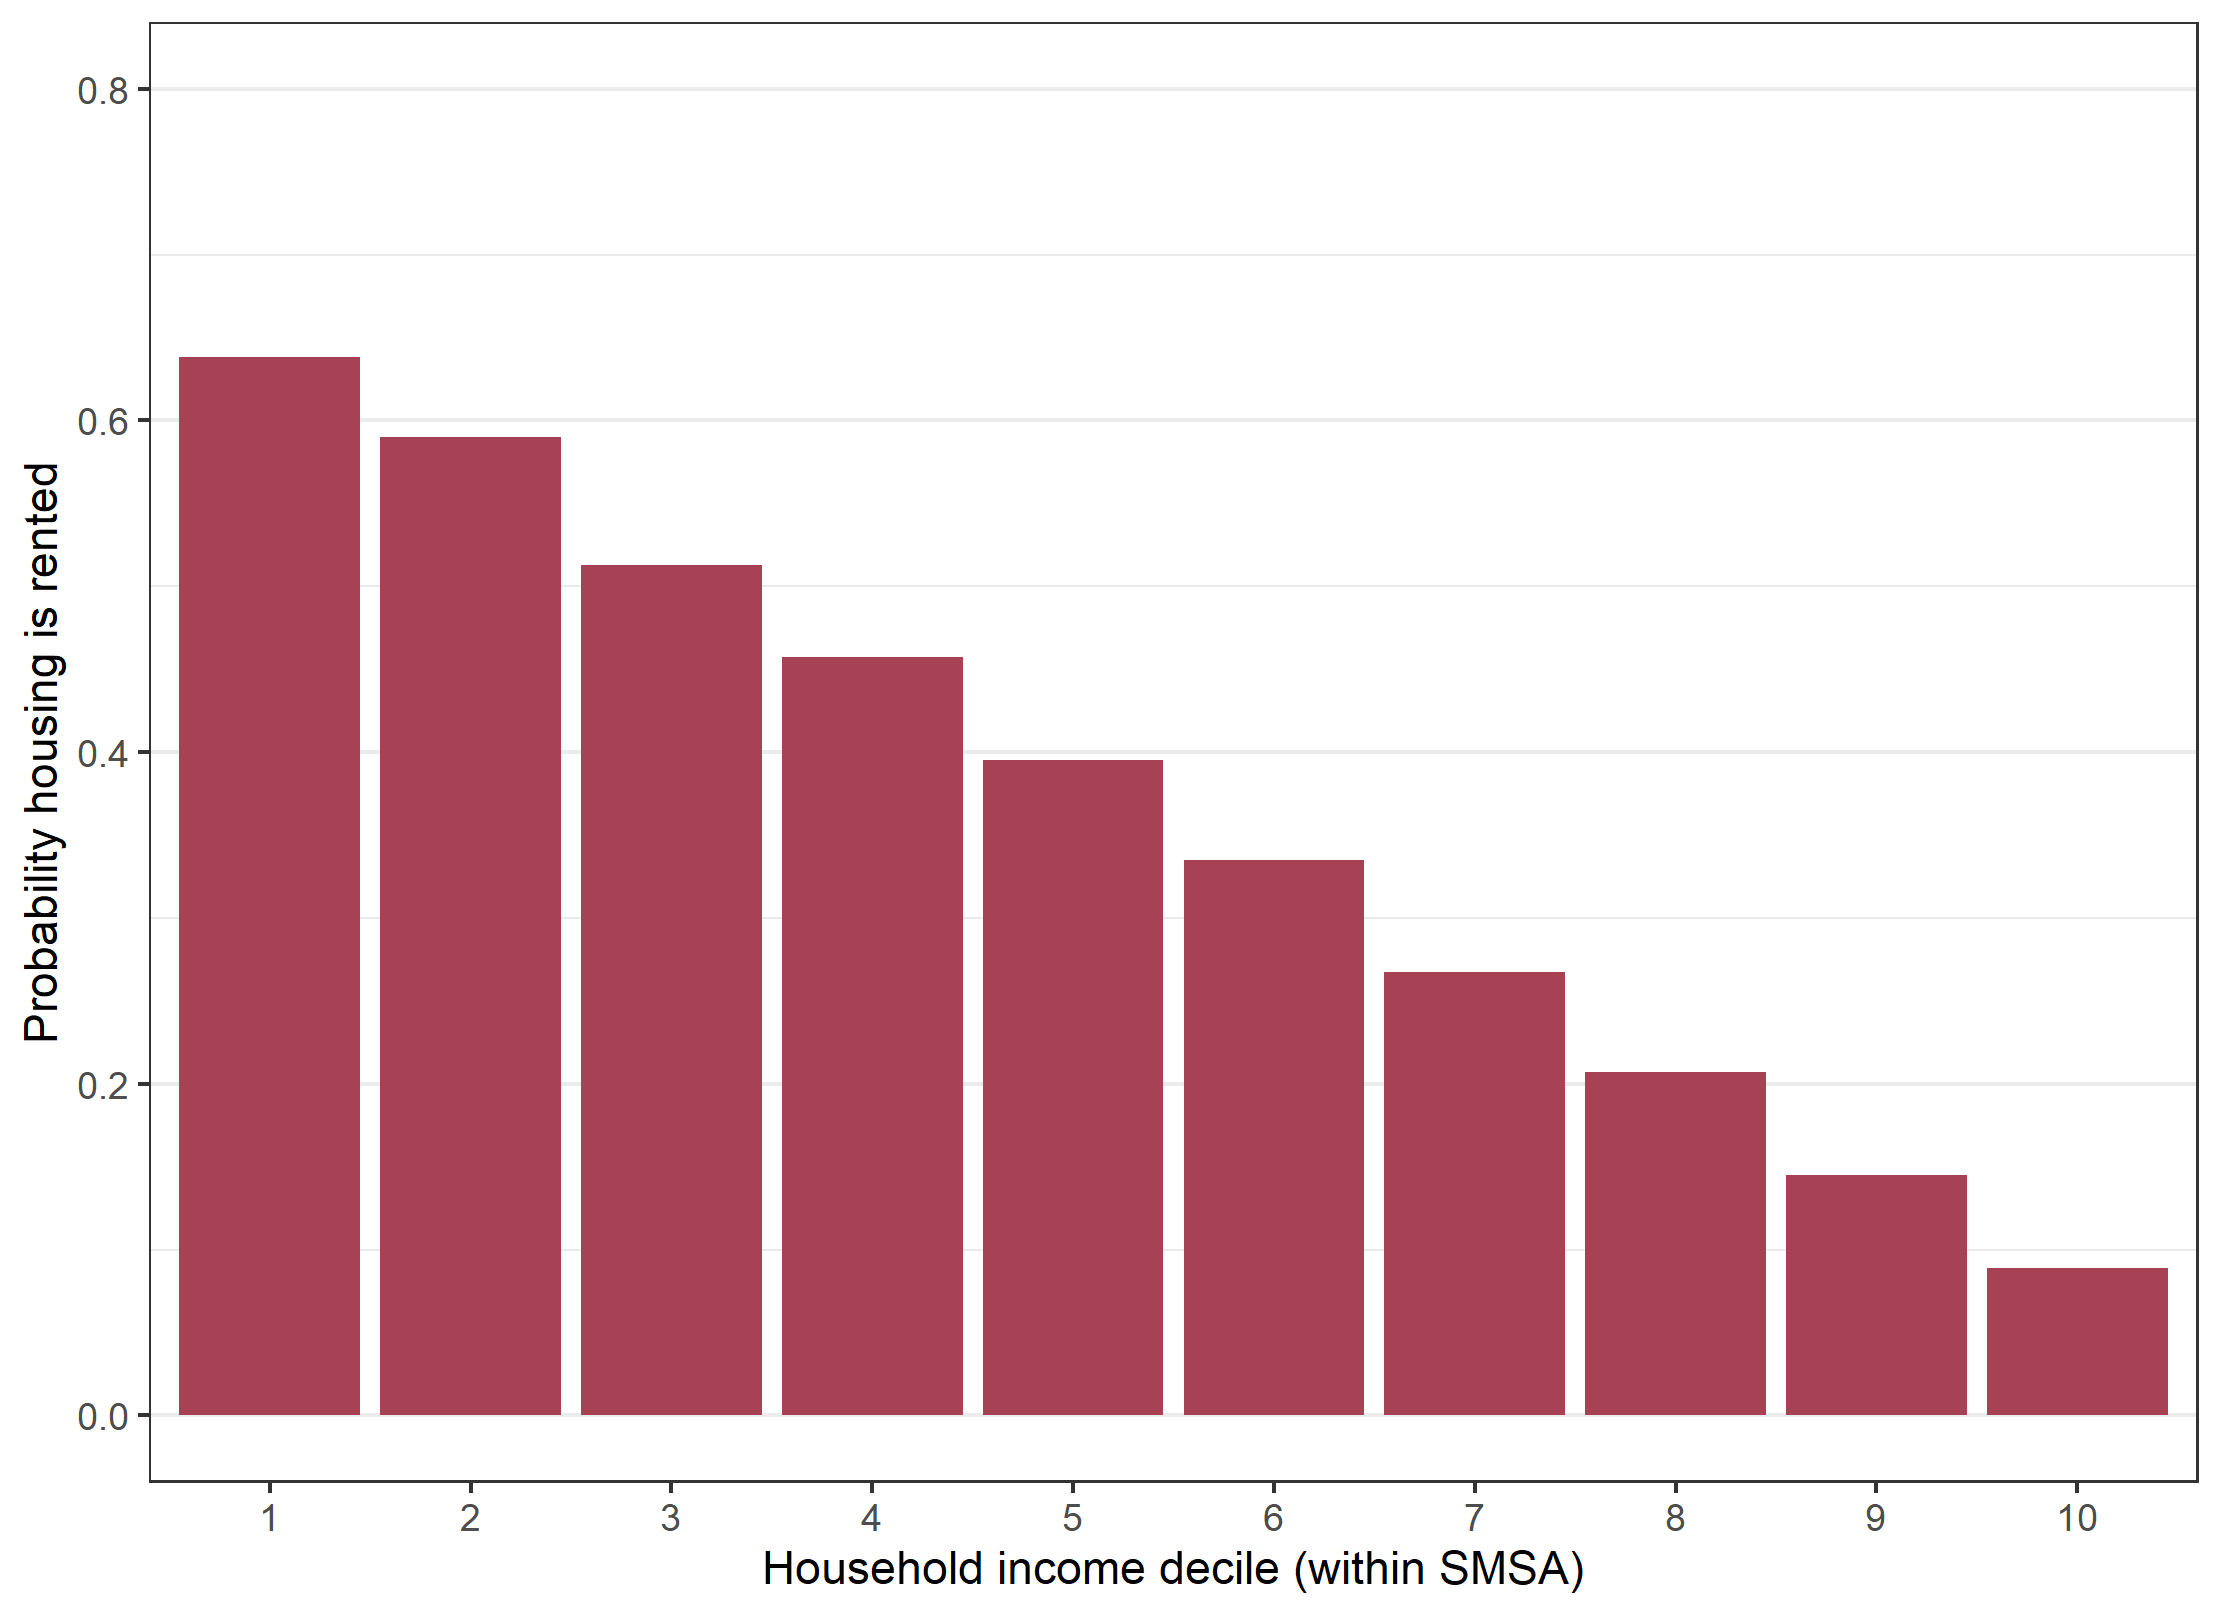
\includegraphics[width = 0.68\textwidth]{../../input/share_renters.png}
    \end{figure}

    \footnotesize
    Source: American Housing Survey (2011, 2013).
\end{frame}

\begin{frame}
    \frametitle{Motivation}
    
    Recently, MW policies in the US have been instituted by sub-national jurisdictions.
    \begin{itemize}
        \item By December 2019: 30 states, 9 counties and 35 cities
        %% substate levels above state ones
        \item Typically, workers face different MW levels at workplace and residence locations \textit{within cities}
    \end{itemize}
    
    \vspace{2mm}
    Conceptualize MW levels as \textit{place-based} policies.
    \begin{itemize}
        \item Commuting patterns matter $\Rightarrow$ Expect rent effects in residence locations 
        of workers bound by the policy
        \item Long-run: workers sort to locations close to high MW levels (Not this paper!)
    \end{itemize}
\end{frame}

\begin{frame}
    \frametitle{A motivating example}
    \begin{columns}
        \begin{column}{0.44\textwidth}
            \vspace{-8mm}
            \begin{figure}
                \centering
                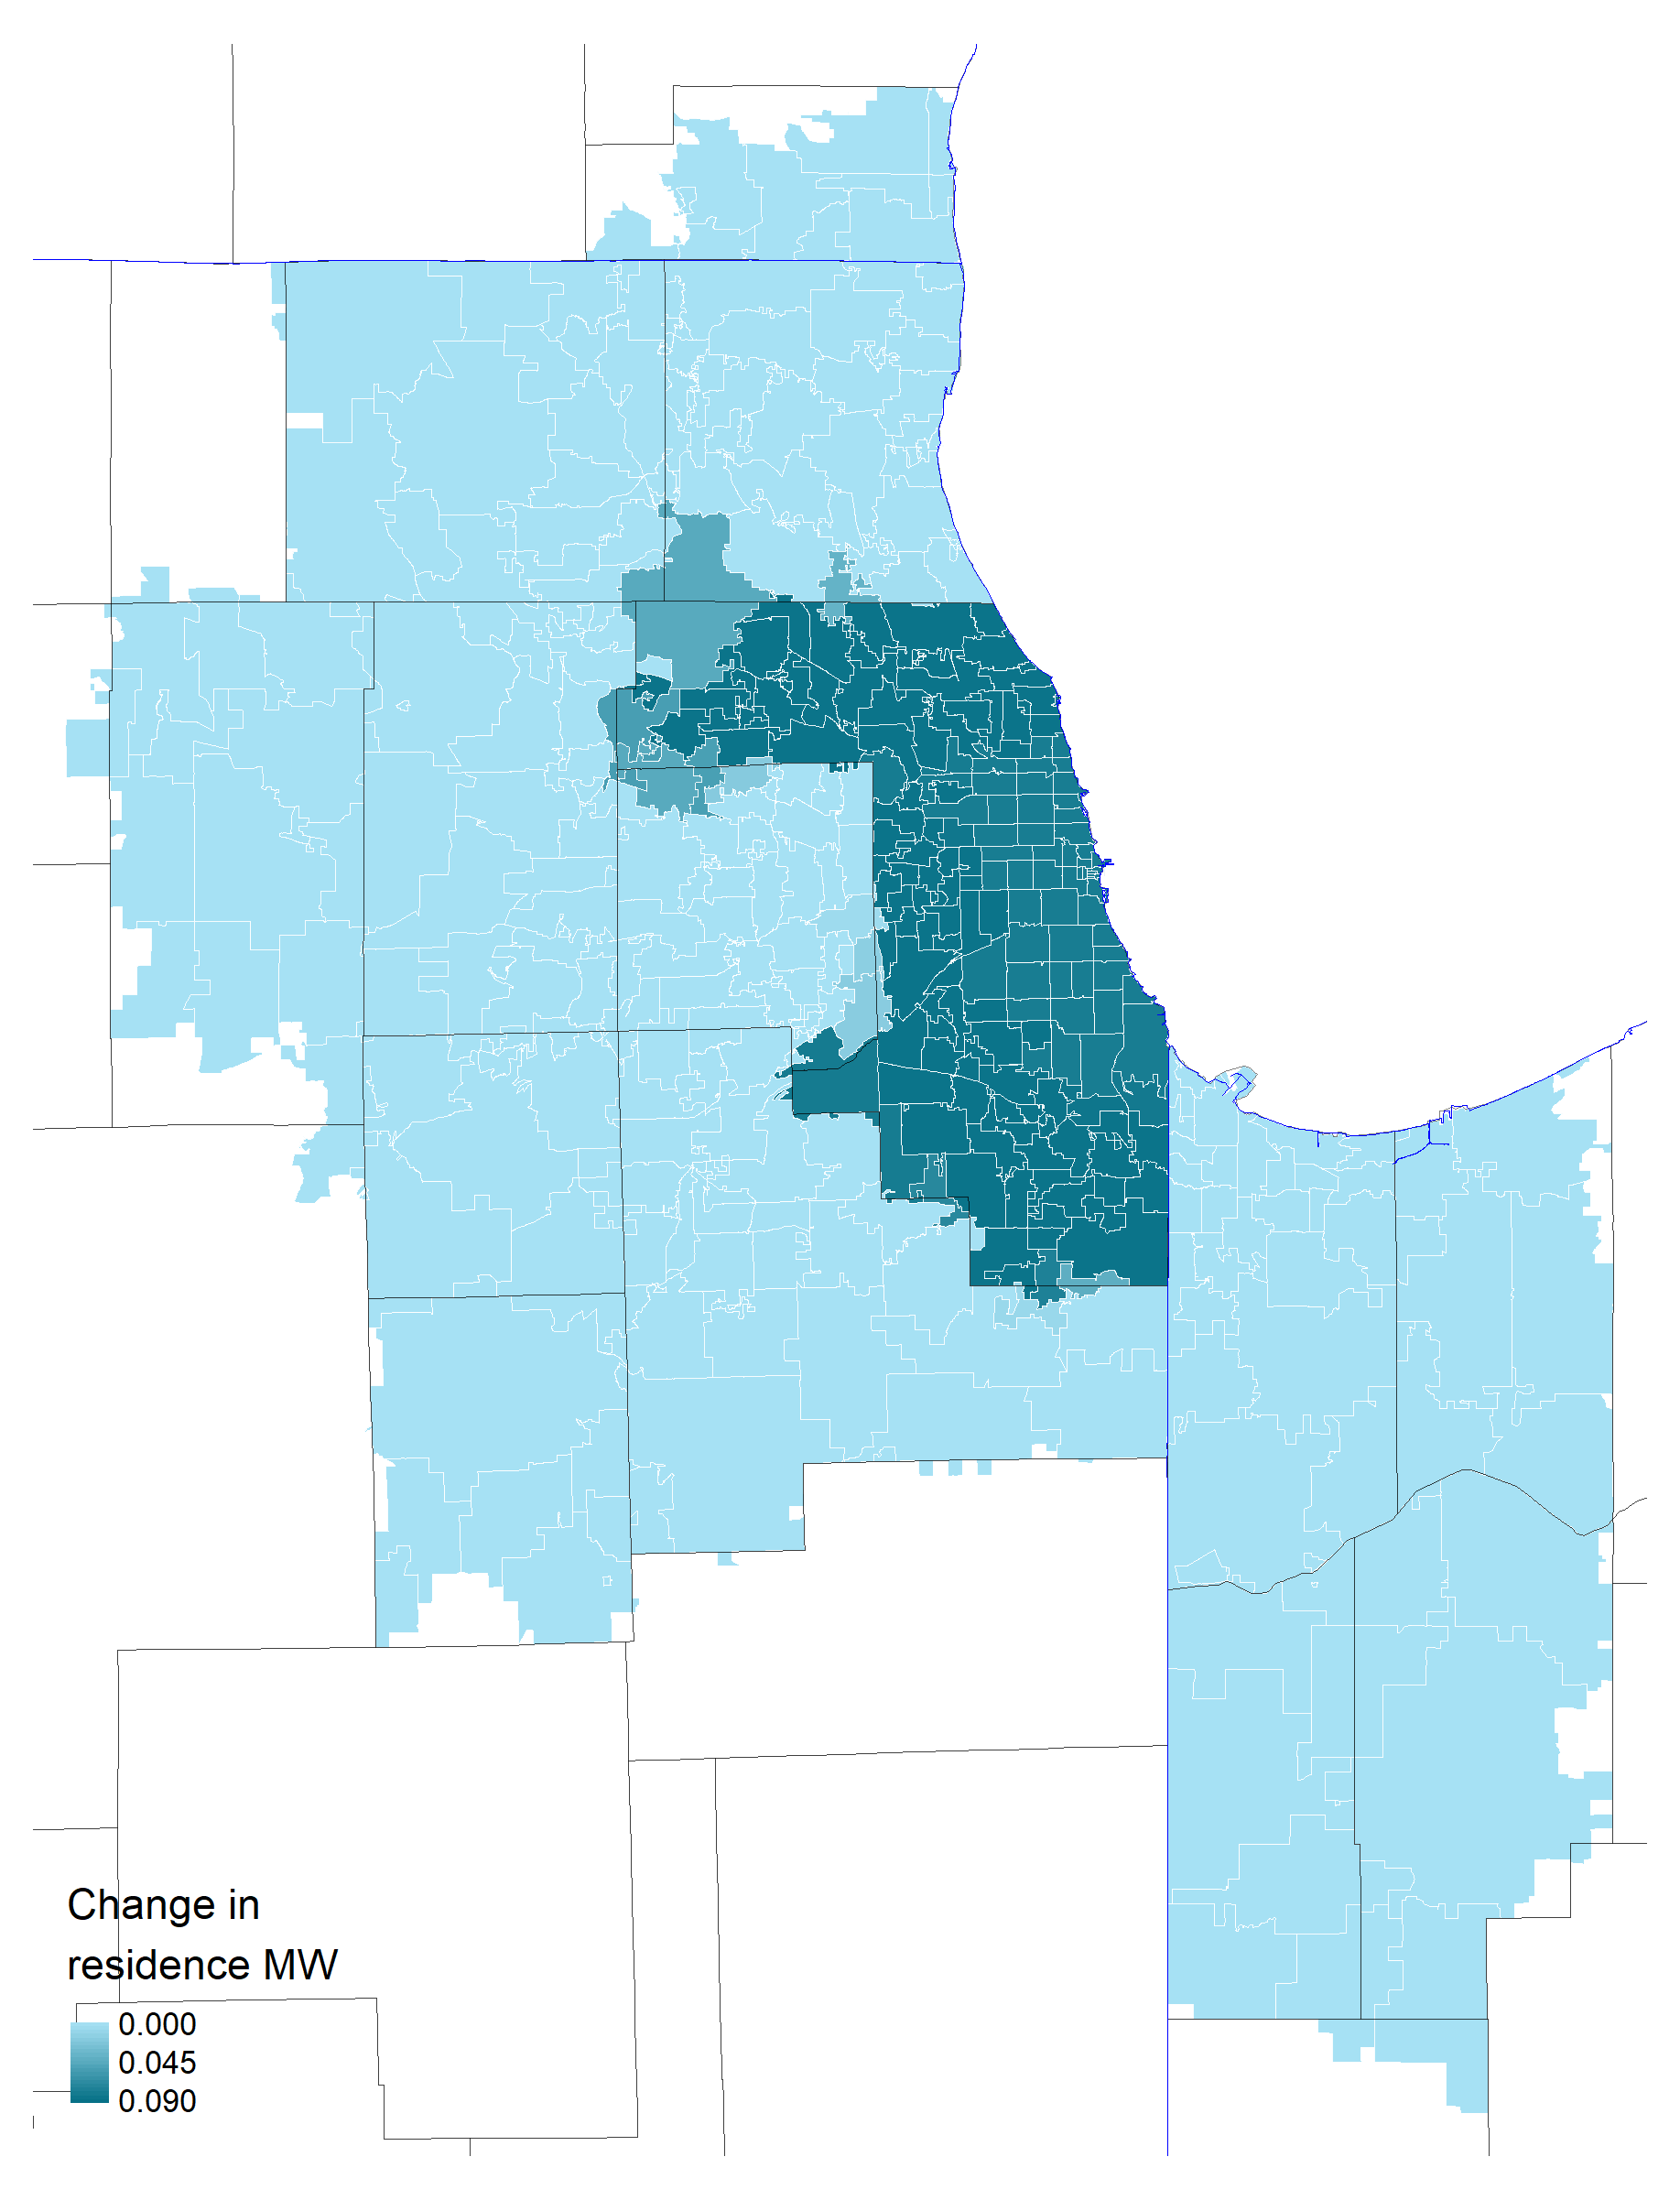
\includegraphics[scale = 0.39]{maps_events/output/chicago_2019-6_statutory_mw.png}
            \end{figure}   
        \end{column}
        \begin{column}{0.56\textwidth}
            Cook County, IL
            \begin{itemize}
                \item Raised local MW from \$12 to \$13 in July 2019. 
                \item State MW is \$8.25 since 2010, and federal MW is \$7.25 since 2009.
                \vspace{2mm}
                \pause
                \item A model where only same-location MW affects rents 
                would likely miss rent increases outside of Cook County
            \end{itemize}
        \end{column}
    \end{columns}
\end{frame}

\begin{frame}
\frametitle{A novel model-based measure of exposure to minimum wages}

    For ZIP code $i$ and month $t$ we define the {\color{blue} workplace MW} as
    $$
    {\color{blue} \mw^{\wkp}_{it}} = 
    \sum_{z \in \Z(i)} \pi_{i z} \ln \MW_{zt} \ ,
    $$
    where
    \vspace{1mm}
    \begin{itemize} \small
        \item $\MW_{zt}$ is statutory MW in $z$ at time $t$
        \item $\Z(i)$ are workplace locations of $i$'s residents
        \item $\pi_{i z} = L_{i z}/L_i$ is the share of $i$'s residents who work 
        in $z$
    \end{itemize}

    \vspace{4mm}
    The {\color{red} residence MW} is simply
    $$
    {\color{red} \mw^{\res}_{it}} = \ln \MW_{it} .
    $$
\end{frame}

\begin{frame}[label = chi_example]
    
    \vspace{-5mm}
    \begin{columns}
        \begin{column}{0.50\textwidth}
            \vspace{-4mm}
            \begin{figure}
                \centering
                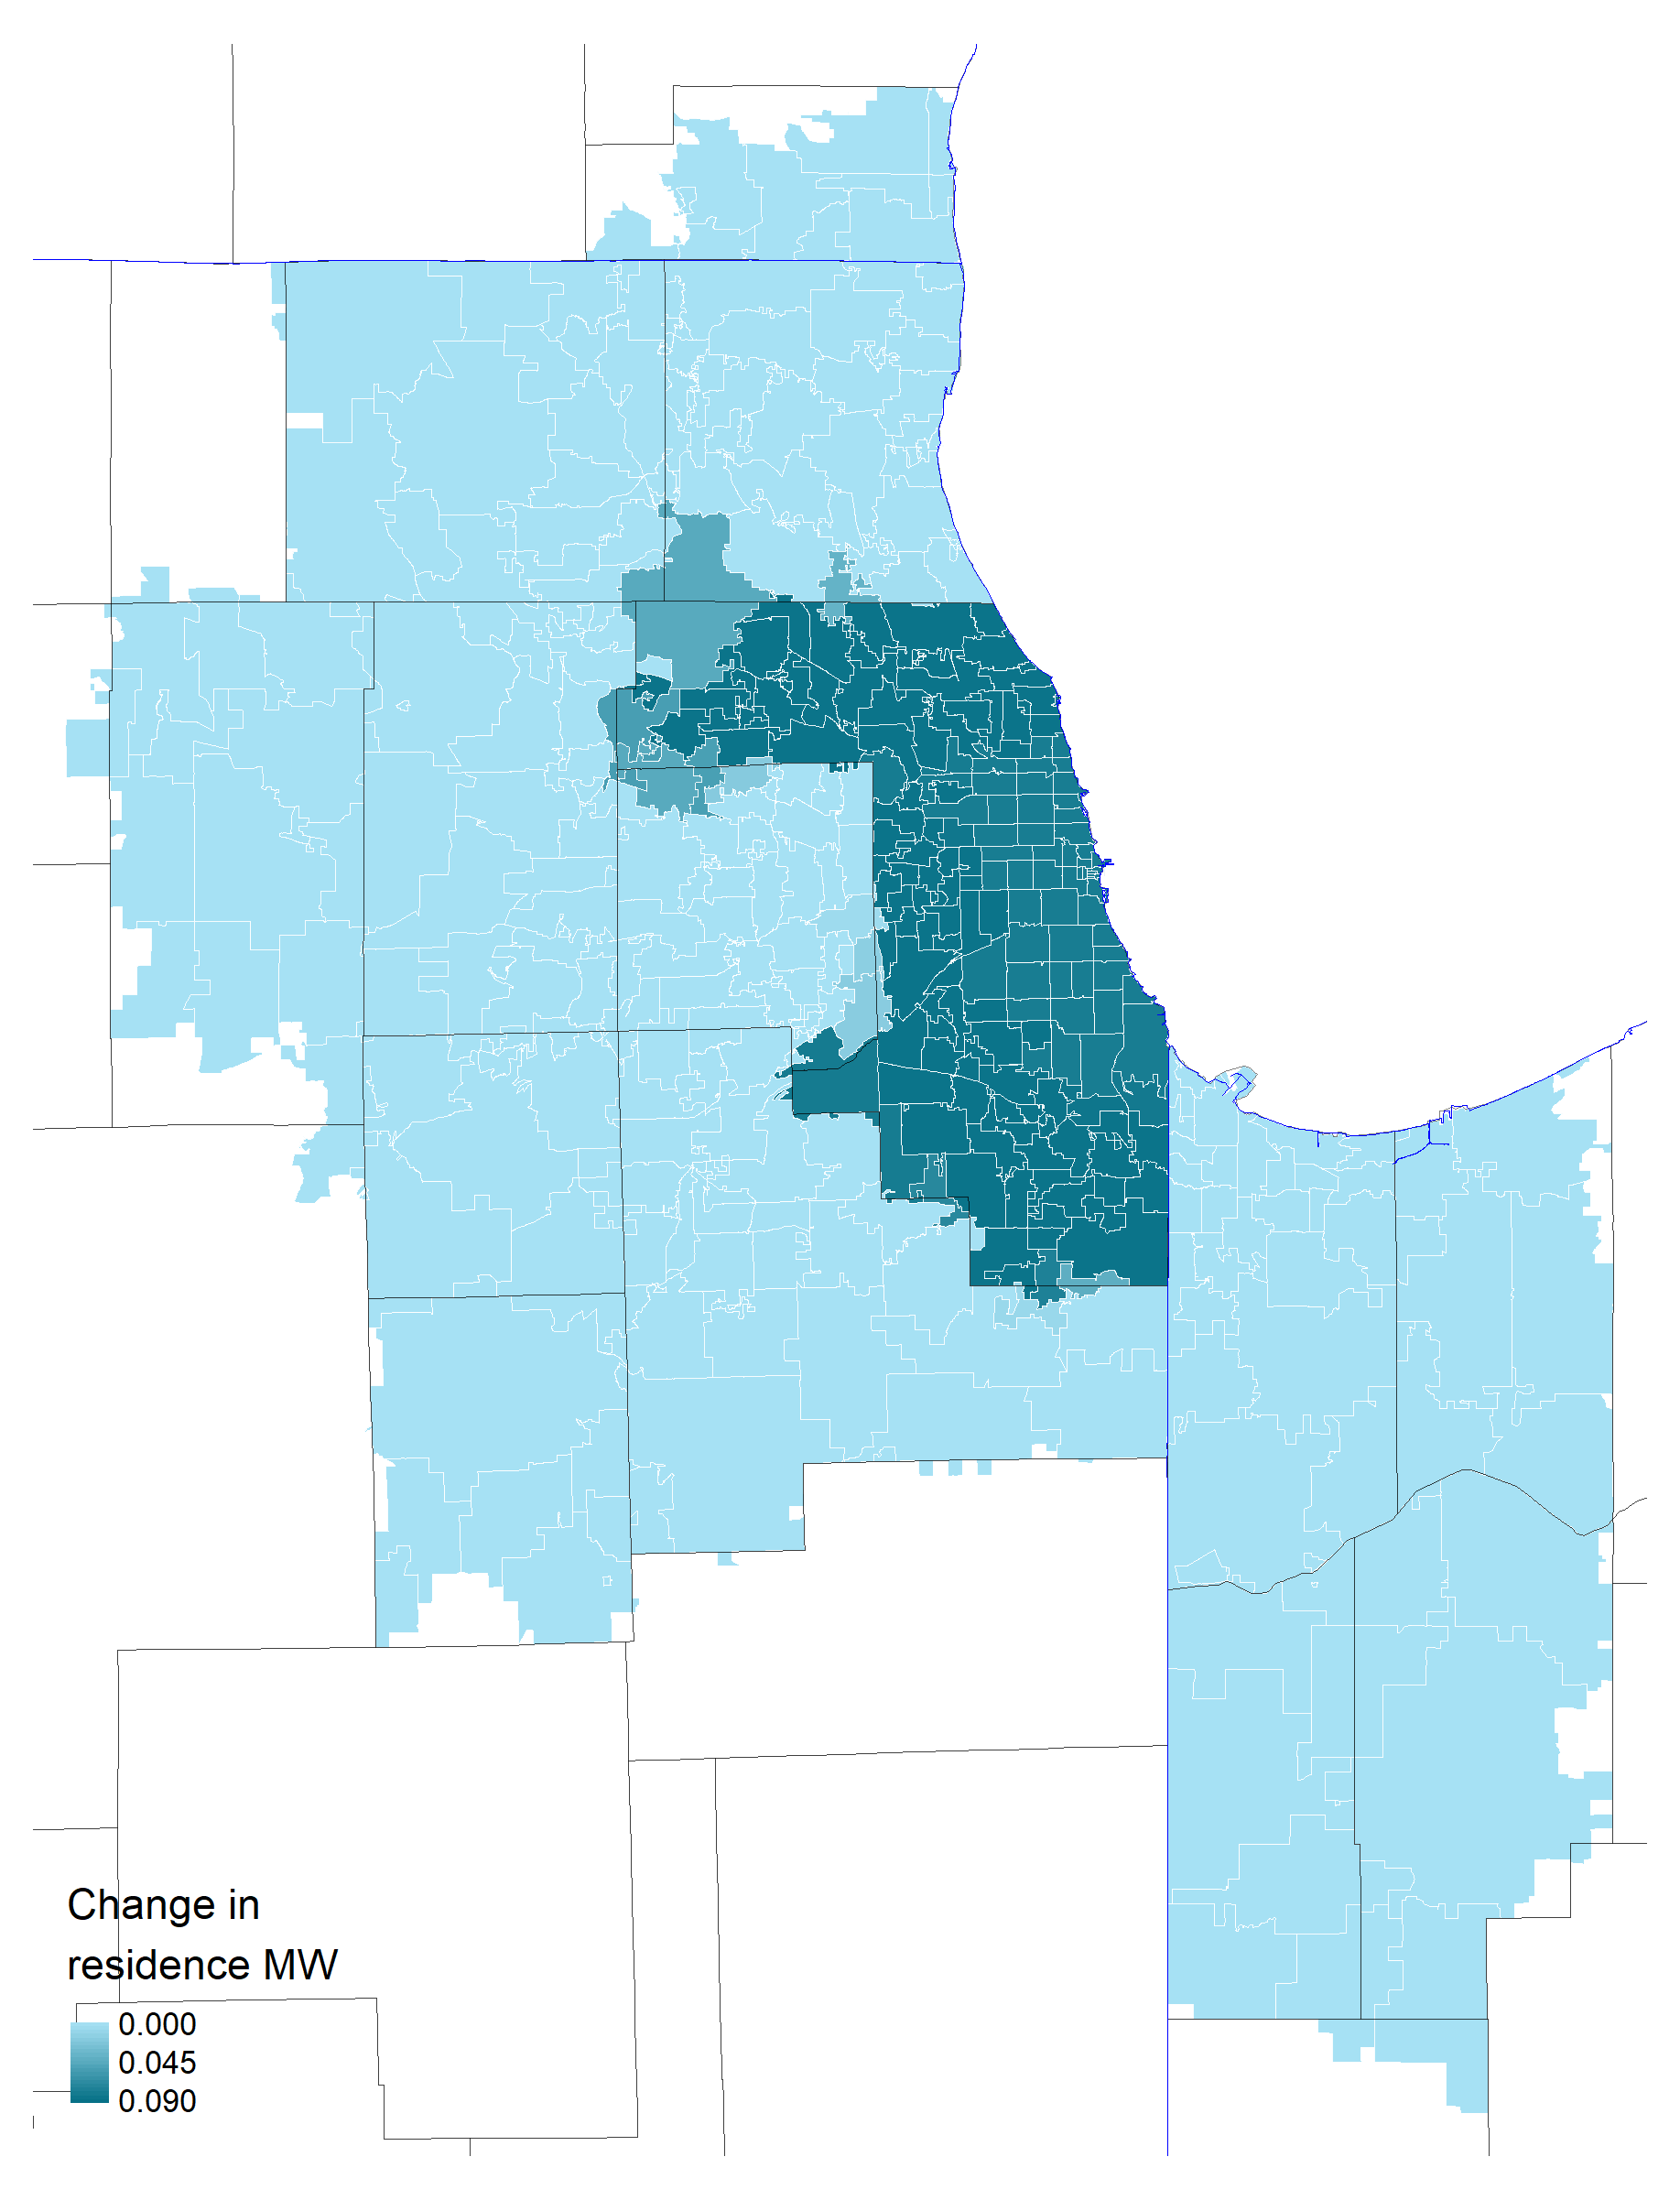
\includegraphics[scale = 0.395]{maps_events/output/chicago_2019-6_statutory_mw.png}
            \end{figure}   
        \end{column}
        \begin{column}{0.50\textwidth}
            \vspace{-4mm}
            \begin{figure}
                \centering
                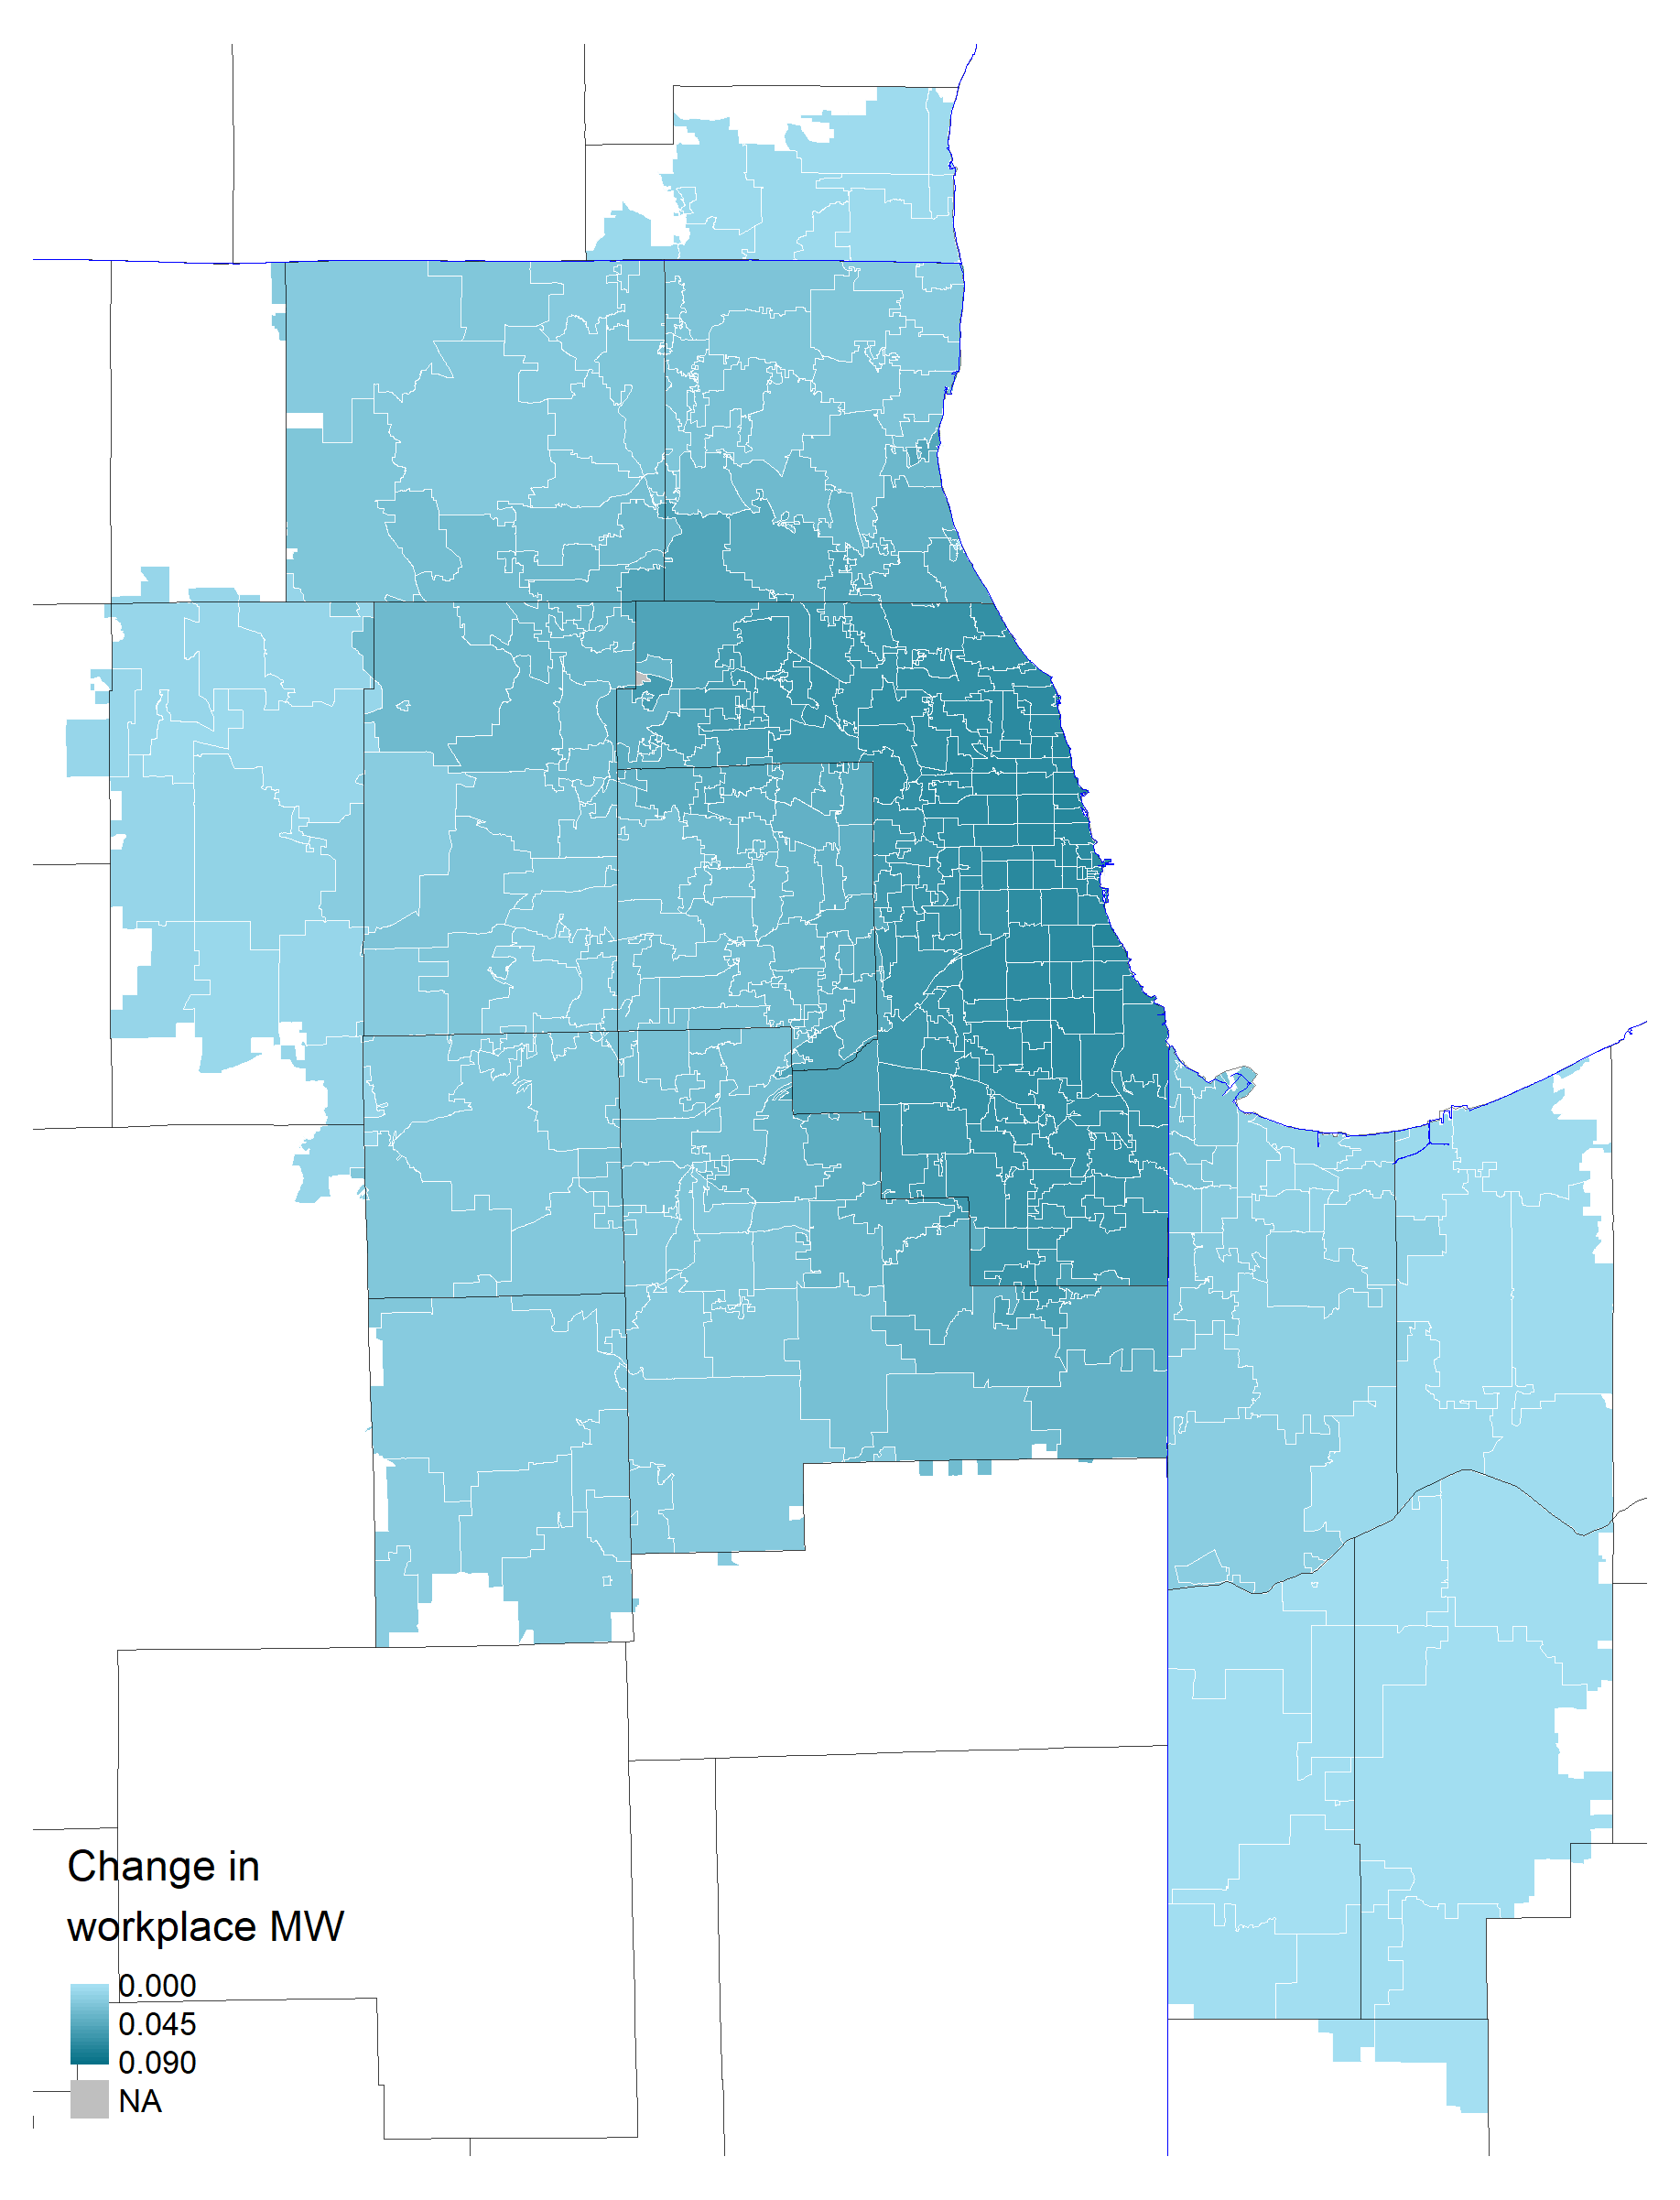
\includegraphics[scale = 0.395]{maps_events/output/chicago2019-6_wkp_mw.png}
            \end{figure}   
        \end{column}
    \end{columns}
    \vspace{3mm}
    \hyperlink{nyc_example}{\beamerbutton{NYC}} 
    \hyperlink{bay_example}{\beamerbutton{Bay Area}}
    \hyperlink{san_diego_example}{\beamerbutton{San Diego}}
    \hyperlink{kc_example}{\beamerbutton{Kansas City}}
\end{frame}


\begin{frame}
    \frametitle{This paper}
    
    What we do
    \begin{itemize}
        \vspace{.5mm} \item Accounting for spatial spillovers, estimate 
        elasticity of rents in the local housing market to
         {\color{blue} workplace MW} and {\color{red} residence MW} changes
        \vspace{.5mm} \item Estimate share of the extra dollar generated by a
        counterfactual MW increases pocketed by landlords in each local market
    \end{itemize}
    
    \vspace{3mm}
    \pause
    How we do it
    \begin{itemize}
        \vspace{.5mm} \item Exploit high-frequency (month) high-resolution 
        (ZIP code) rents data from Zillow
        \vspace{.5mm} \item Construct novel dataset of MW policies at ZIP code level
        \vspace{.5mm} \item Propose a novel measure of exposure to MW changes 
        based on commuting shares
    \end{itemize}
\end{frame}

\begin{frame}
    \frametitle{Preview of findings}
    
    Main estimation results
    \begin{itemize}
        \vspace{1mm}
        \item $\uparrow$ 10 percent in {\color{blue} workplace MW}
        $\implies$ $\uparrow$ 0.55 percent in rents
        \vspace{1mm}
        \item $\uparrow$ 10 percent in {\color{red} residence MW}
        $\implies$ $\downarrow$ 0.21 percent in rents
        \vspace{1mm}
        \item $\uparrow$ 10 percent in both measures $\implies$ $\uparrow$ 0.34 percent in rents
    \end{itemize}
    %% Similar magnitude to estimates of MW effects on prices
    
    \vspace{5mm}
    \pause
    Counterfactual increase in federal MW from \$7.25 to \$9 in highly affected areas
    \begin{itemize}
        \vspace{1mm}
        \item Rent changes vary between $-0.4$ to $0.75$ percent (median $0.5$ percent)
        % A rental that costs 2000 would increase to 2100
        \vspace{1mm}
        \item Share pocketed by landlords is between $-15$ and $17$ cents (median $10$ cents)
    \end{itemize}
    %% Distribution are left skewed or negatively skewed
\end{frame}

\begin{frame}
    \frametitle{Outline for Today}
    \tableofcontents[hideallsubsections]
\end{frame}

%%%%%%%%%%%%%%%%%%%%%%%%%%%%%%%%%%%%%%%%%%%%%%%%%%%%%%%%%%%%%%%%%%%%%%%%%%%%%%%%
\section{Partial Equilibrium Model (intuition)}

\begin{frame}
    \frametitle{Overview}
    
    Goals of the model:
    \begin{itemize}
        \item Stylized answer to what is the effect of MW changes on rents
        \item Motivate and derive a new measure of exposure to MW
    \end{itemize}
    
    \pause
    \vspace{3mm}
    Assumptions:
    \begin{itemize}
        \item A higher MW increases income, which \textit{increases} housing demand
        \item A higher MW increases non-tradable consumption prices, which \textit{decreases} housing demand
        \item Static model, so residence and workplace locations of workers are fixed
    \end{itemize}

    \vspace{2mm}
    These assumptions are consistent with the literature.

\end{frame}

\begin{frame}
    \frametitle{Comparative statics}
    
    \begin{columns}
        \begin{column}{0.35\textwidth}
            \begin{enumerate}
                \item Equilibrium in ZIP code $i$
                \item \onslide<2->{\color{blue} MW increases in some $z$}
                \item \onslide<3->{\color{red} MW increases in $i$}
            \end{enumerate}
        \end{column}
        \begin{column}{0.65\textwidth}
            \vspace{-2mm}
            \begin{figure}

                \begin{tikzpicture}[scale=.95]
                
                % Axis
                \draw[->, thick] (0,0) -- (6.5,0);
                \draw[->, thick] (0,0) -- (0,6.2);
                \node[left] at (0.2,6.5) {Rents};
                \node[right] at (5,-0.5) {Square feet};
                
                % Base demand and Supply Curves
                \draw (0.3,4.5) -- (4.8,0.5);
                \draw plot [smooth, tension = 1] coordinates {(0.3,1.4) (3,2.8) (5,4.7)};
                       
                \node[right] at (4.8,0.5) {$H\left(R_i, P_i^1, \{Y_z^1\}\right)$};
                \node[right] at (5,4.7) {$S\left(R_i\right)$};
                
                % Base Eq
                \def\x{2.541}
                \def\y{2.501}
                \draw[dashed] (\x,0) -- (\x,\y);
                \draw[dashed] (0,\y) -- (\x,\y);
                \node[below] at (\x-.1,0) {$H_1^*$};
                \node[left] at (0,\y-.1) {$R_1^*$};
                \only<1>{
                    \filldraw[black] (\x,\y) circle (1pt);
                }
                
                
                % Equilibrium 2 - Wkp MW increases
                \def\xOne{3.535}
                \def\yOne{3.215}
                \only<2>{
                    \draw[color = blue] (0.3,6.1) -- (4.8,2.1);
                    \node[right] at (4.8,2.1) {$H\left(R_i, P_i^1, {\color{blue}\{Y_z^2\}}\right)$};

                    \draw[dashed, color = blue] (\xOne,0) -- (\xOne,\yOne);
                    \draw[dashed, color = blue] (0,\yOne) -- (\xOne,\yOne);
                    \node[below, color = blue] at (\xOne,0) {$H_2^*$};
                    \node[left, color = blue] at (0, \yOne) {$R_2^*$};

                    \filldraw[blue] (\xOne,\yOne) circle (1pt);
                }

                % Equilibrium 3 - Res MW increases
                \def\xTwo{3.05}
                \def\yTwo{2.85}
                \only<3>{
                    \draw[dashed, color = blue] (0.3,6.1) -- (4.8,2.1);
                    \draw[color = red] (0.3,5.3) -- (4.8,1.3);
                    \node[right] at (4.8,1.3) {$H\left(R_i, {\color{red}P_i^3}, {\color{red}\{Y_z^3\}}\right)$};

                    \draw[dashed, color = blue] (\xOne,0) -- (\xOne,\yOne);
                    \draw[dashed, color = blue] (0,\yOne) -- (\xOne,\yOne);
                    \node[below, color = blue] at (\xOne+.1,0) {$H_2^*$};
                    \node[left, color = blue] at (0, \yOne+.2) {$R_2^*$};

                    \draw[dashed, color = red] (\xTwo,0) -- (\xTwo,\yTwo);
                    \draw[dashed, color = red] (0,\yTwo) -- (\xTwo,\yTwo);
                    \node[below, color = red] at (\xTwo,0) {$H_3^*$};
                    \node[left, color = red] at (0,\yTwo+.1) {$R_3^*$};
                    
                    \filldraw[red] (\xTwo,\yTwo) circle (1pt);
                }
                
                \end{tikzpicture}
                
            \end{figure}
        \end{column}
    \end{columns}

\end{frame}

\begin{frame}
    \frametitle{Representation}

    In this model, assuming homogeneity across workplace locations of
    \begin{enumerate}
        \item elasticity of per-person housing demand to income, and
        \item elasticity of income to the MW
    \end{enumerate}
    we obtain
    \[
    \Delta \text{log rents} = \underbrace{\beta_i}_{\ge 0} \times \Delta {\color{blue}  \text{workplace MW}}
                            + \underbrace{\gamma_i}_{< 0}  \times \Delta {\color{red} \text{residence MW}}
    \]

    \vspace{3mm}
    \pause
    Discussion:
    \begin{itemize}
        \item Assumption (1) would hold for homothetic preferences
        \item In estimation can allow for heterogeneity as long as not correlated with MW changes
    \end{itemize}

\end{frame}


%%%%%%%%%%%%%%%%%%%%%%%%%%%%%%%%%%%%%%%%%%%%%%%%%%%%%%%%%%%%%%%%%%%%%%%%%%%%%%%%
\section{Data}

\begin{frame}[label = zillow_data]
    \frametitle{Zillow Data}
    
    Collect \textit{median per-square-foot rents} at ZIP code and month levels for several housing categories.
        
    \pause
    \vspace{2mm}
    We use category single-family, condominium, and cooperative houses (SFCC).
    \begin{itemize}
        \item Most populated series in Zillow
        \item We also estimate our models with other housing categories
    \end{itemize}
        
    \vspace{2mm}
    Limitation: Zillow sample is not random.

    \hyperlink{zillow_pop_density}{\beamerbutton{Zillow ZIP Codes and Population Density}}
\end{frame}

\begin{frame}[label=stat_MW]
    \frametitle{The Statutory MW}
    
    Collect MW data at state, county and city levels between Jan 2010 and Dec 2019.
    
    \vspace{2.5mm}
    Spatial match:
    \begin{itemize}
        \item Assign USPS ZIP codes to census blocks based on blocks' centroids
        \item Add matching of places, counties, and states using census crosswalk
    \end{itemize}
    
    \vspace{2.5mm}
    Assign MWs to each block and define statutory MW as maximum between city, 
    county, state, and federal leves.
    
    \vspace{2.5mm}
    Define the statutory MW in ZIP code $i$ and month $t$, $\MW_{it}$, as weighted
    average of statutory MWs at block, using housing units as weights.
    %% Some ZIP codes don't have housing units --> arithmetic mean

    \vspace{2mm}
    \hyperlink{dist_mw_changes}{\beamerbutton{Distribution of (positive) MW changes}}
    \hyperlink{mw_changes_map}{\beamerbutton{US map of decennial MW changes}}
\end{frame}

\subsection{MW measures}

\begin{frame}
    \frametitle{Constructing the MW measures}
        
    Collect data from LEHD Origin-Destination Employment Statistics (LODES) for years 2009--18.
    \begin{itemize}
        \item Origin-destination matrices at block level constructed from tax records
    \end{itemize}

    \vspace{1mm}
    Construct \textbf{origin-destination matrix} at ZIP code level using spatial match.
    
    \pause
    \vspace{2mm}
    Define the MW measures as before:
    $$
    {\color{blue} \mw^{\wkp}_{it}} = \sum_{z \in \Z(i)} \pi_{i z} \ln \MW_{zt}
    \quad\quad\text{and}\quad\quad
    {\color{red} \mw^{\res}_{it}} = \ln \MW_{it}
    $$

    \vspace{2mm}
    In our baseline specification we use constant commuter shares for all workers as of 2017.

\end{frame}

%%%%%%%%%%%%%%%%%%%%%%%%%%%%%%%%%%%%%%%%%%%%%%%%%%%%%%%%%%%%%%%%%%%%%%%%%%%%%%%%
\section{Empirical Strategy and Results}

\begin{frame}
    \frametitle{Empirical model}
        
    We estimate versions of the following empirical model:
    \[
    \Delta r_{it} = \delta_t +
        \beta \Delta {\color{blue}\mw^{\wkp}_{it}} +
        \gamma \Delta {\color{red}\mw^{\res}_{it}} + 
        \Delta \mathbf{X}^{'}_{it} \eta + 
        \Delta \varepsilon_{it} 
    \]
    where $r_{it} = \ln R_{it}$ and $\mathbf{X}^{'}_{it}$ are time-varying controls.
    
    \pause
    \vspace{3mm}
    For causal effect of $\beta$ and $\gamma$ we need strict exogeneity
    $$
    E\left[
        \begin{pmatrix}
            \Delta {\color{blue}\mw^{\wkp}_{is}} \\
            \Delta {\color{red}\mw^{\res}_{is}} \\
        \end{pmatrix}
        \Delta \varepsilon_{it}
    \bigg| \delta_t, \Delta \mathbf{X}_{it} \right] =
    \begin{pmatrix}
        0 \\
        0 \\
    \end{pmatrix}
    \quad \forall s\in[\underline T, \overline T]
    $$
    %% Plausible for small geographies

    \pause
    \vspace{2mm}
    Two main concerns:
    \begin{enumerate}
        \item State of local economy drives MW changes and rent changes $\Rightarrow$ controls $\mathbf{X}_{it}$
        \item Trends are not parallel $\Rightarrow$ test including leads and lags of MW variables
    \end{enumerate}

\end{frame}

\begin{frame}[label = static]
    \frametitle{Main results}

    \begin{table}
    \label{tab:static}
    \scalebox{0.8}{
        \begin{tabular}{l*{4}{c}}
            \toprule
            & \multicolumn{1}{c}{\shortstack{Change wkp.\ MW\\$\Delta\mw_{it}^{\wkp}$}}
                & \multicolumn{3}{c}{\shortstack{Change log rents\\$\Delta r_{it}$}} \\ \cmidrule(lr){2-2}\cmidrule(lr){3-5}
                                               & (1)   & (2)   & (3)   & (4)            \\ \midrule
            Change residence MW 
                      $\Delta\mw_{it}^{\res}$  &  #4#  &  #4#  &       &  #4#     \\
                                               & (#4#) & (#4#) &       & (#4#)    \\
            Change workplace MW 
                       $\Delta\mw_{it}^{\wkp}$ &       &       &  #4#  & #4#      \\
                                               &       &       & (#4#) & (#4#)    \\ \midrule
            Sum of coefficients                &       &       &       &  #4#     \\
                                               &       &       &       & (#4#)    \\ \midrule
            County-quarter economic controls   &  Yes  & Yes   & Yes   & Yes      \\
            P-value equality                   &       &       &       & #4#      \\
            R-squared                          &  #4#  &  #4#  &  #4#  & #4#      \\
            Observations                       & #0,#  & #0,#  & #0,#  & #0,#     \\\bottomrule
        \end{tabular}
    }
\end{table}

    
    \vspace{2mm}
    \footnotesize
    Note: Standard errors clustered at the state level throughout.

\end{frame}

\begin{frame}[label = dyn_baseline_plot]
    \frametitle{Including leads and lags of workplace MW}

    \begin{figure}
        \centering
        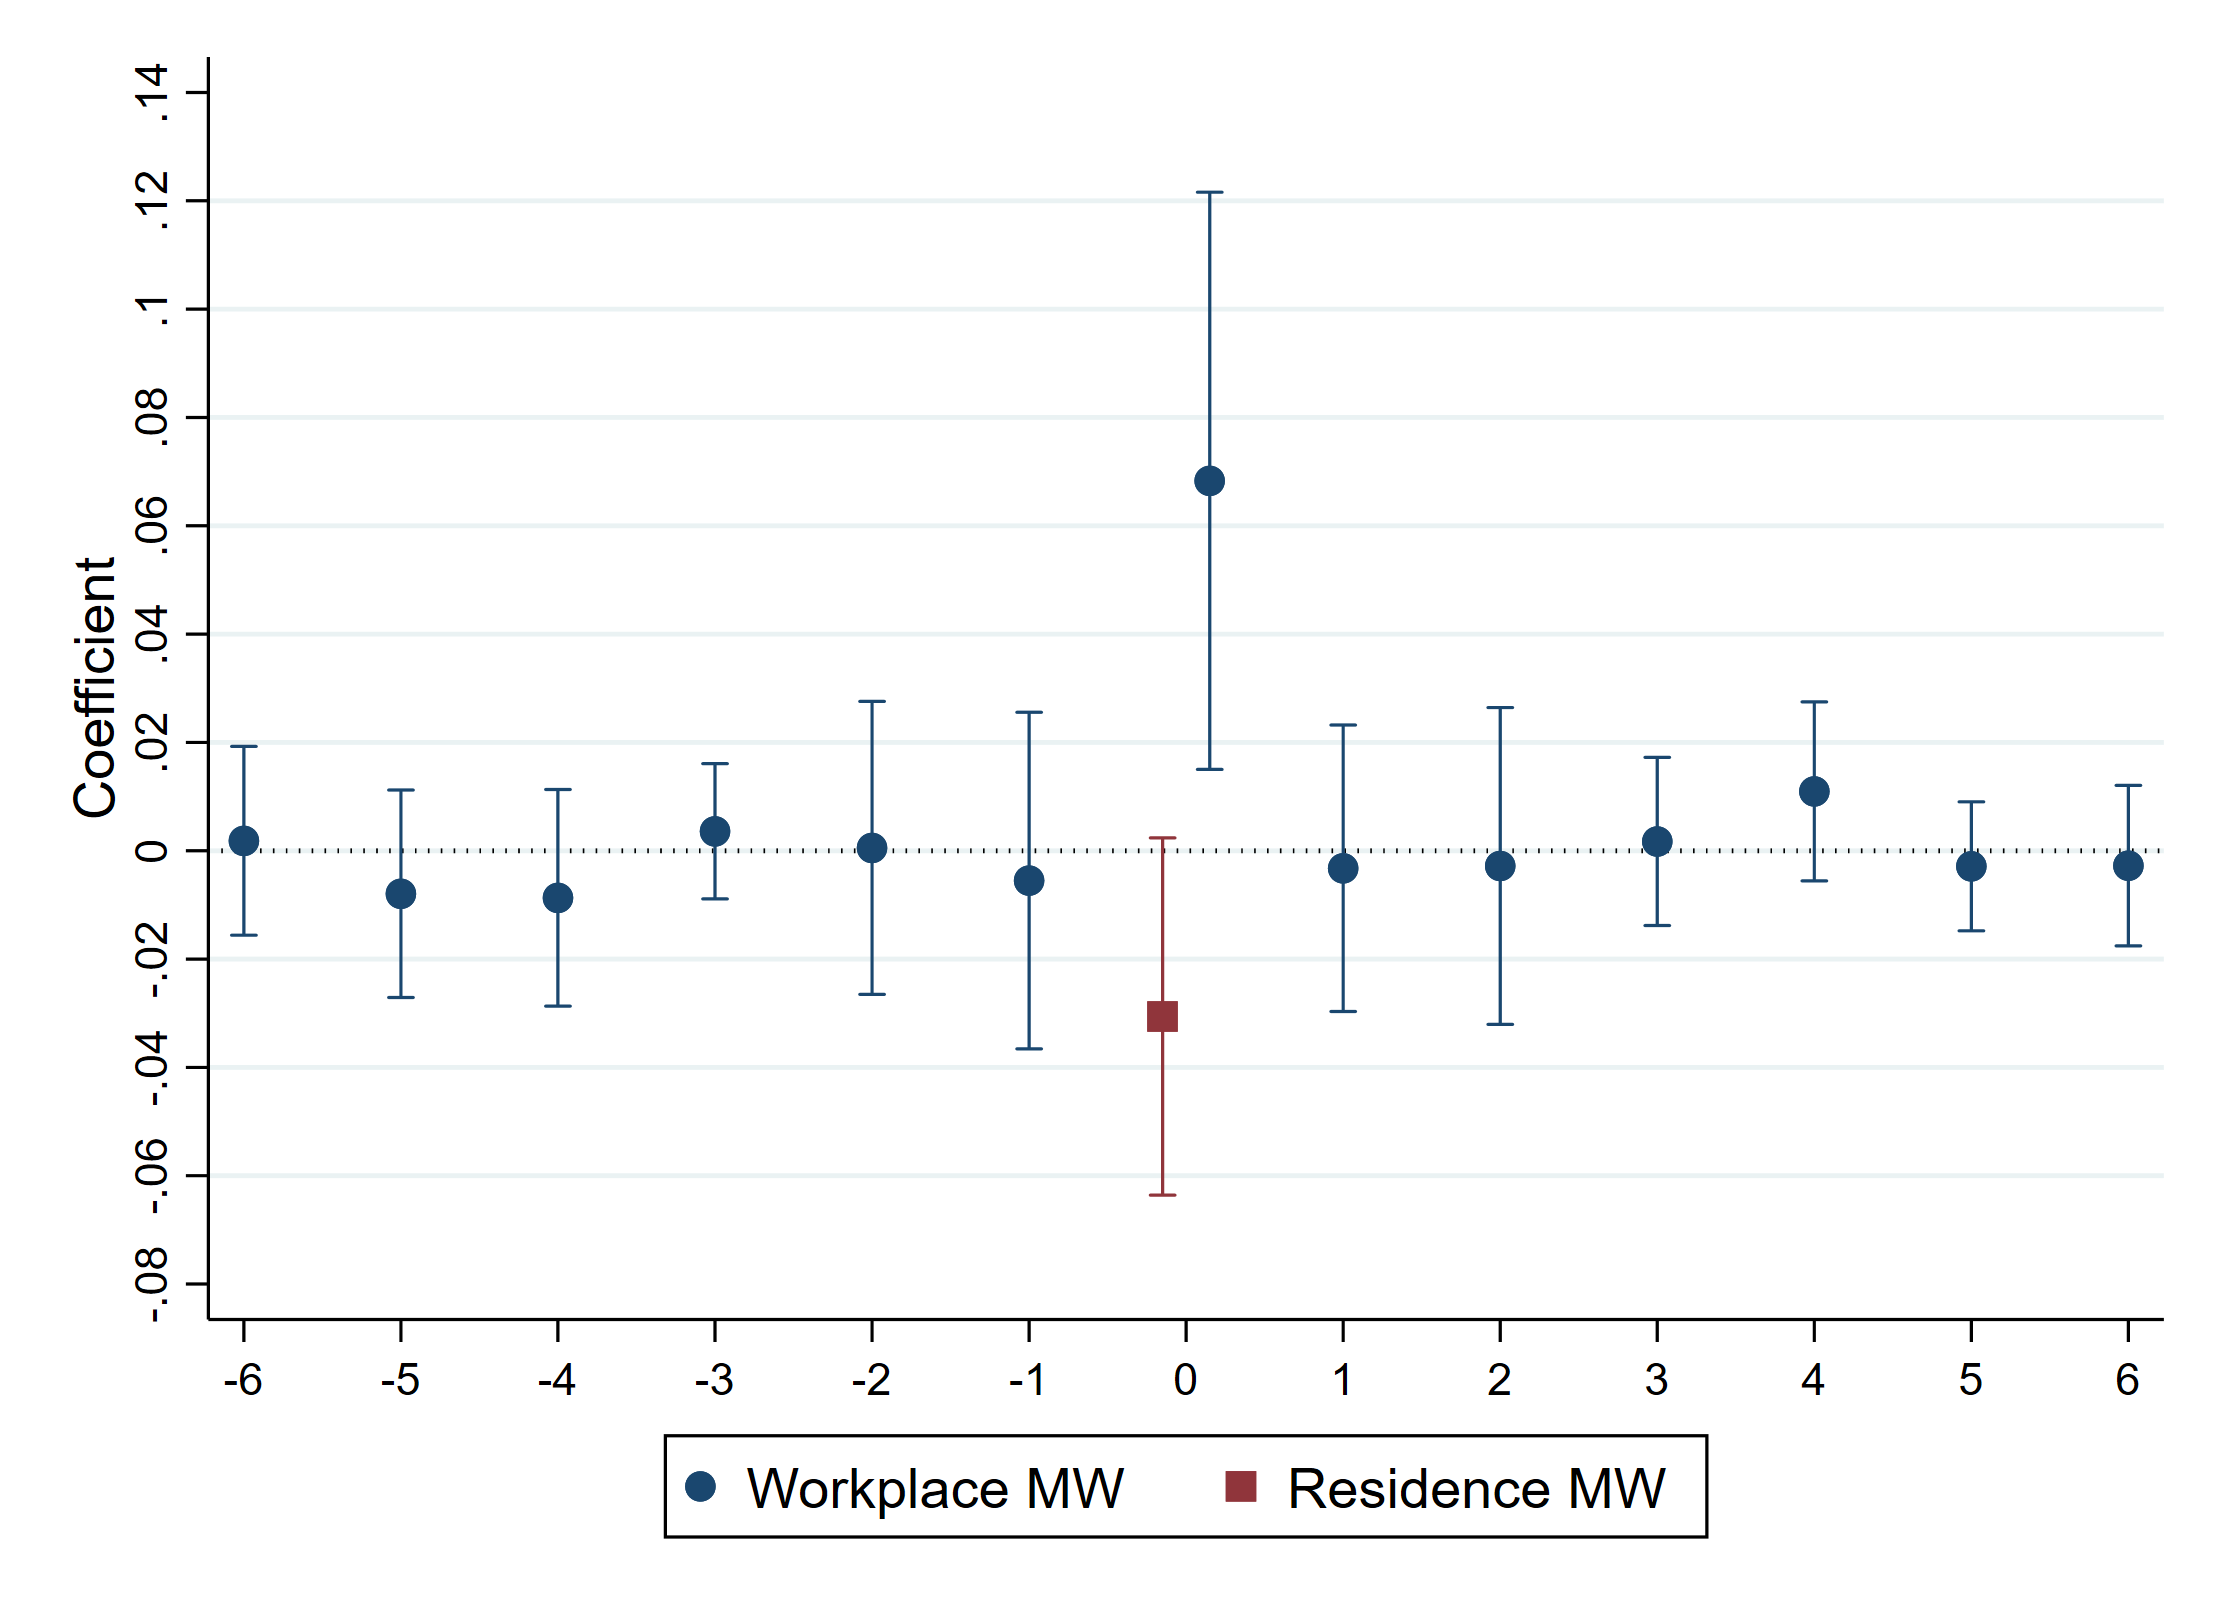
\includegraphics[width=0.68\textwidth]{fd_baseline/output/fd_both_mw_wkp_only_dynamic.png}
    \end{figure}
    
    \hyperlink{exclude_res}{\beamerbutton{Exclude residence MW}}
    \hyperlink{res_only_dyn}{\beamerbutton{Leads and lags of residence MW only}}
    \hyperlink{both_dyn}{\beamerbutton{Leads and lags of both}}
\end{frame}

\begin{frame}[label = dyn_baseline_plot]
    \frametitle{Including leads and lags of workplace MW, after June 2015}

    \begin{figure}
        \centering
        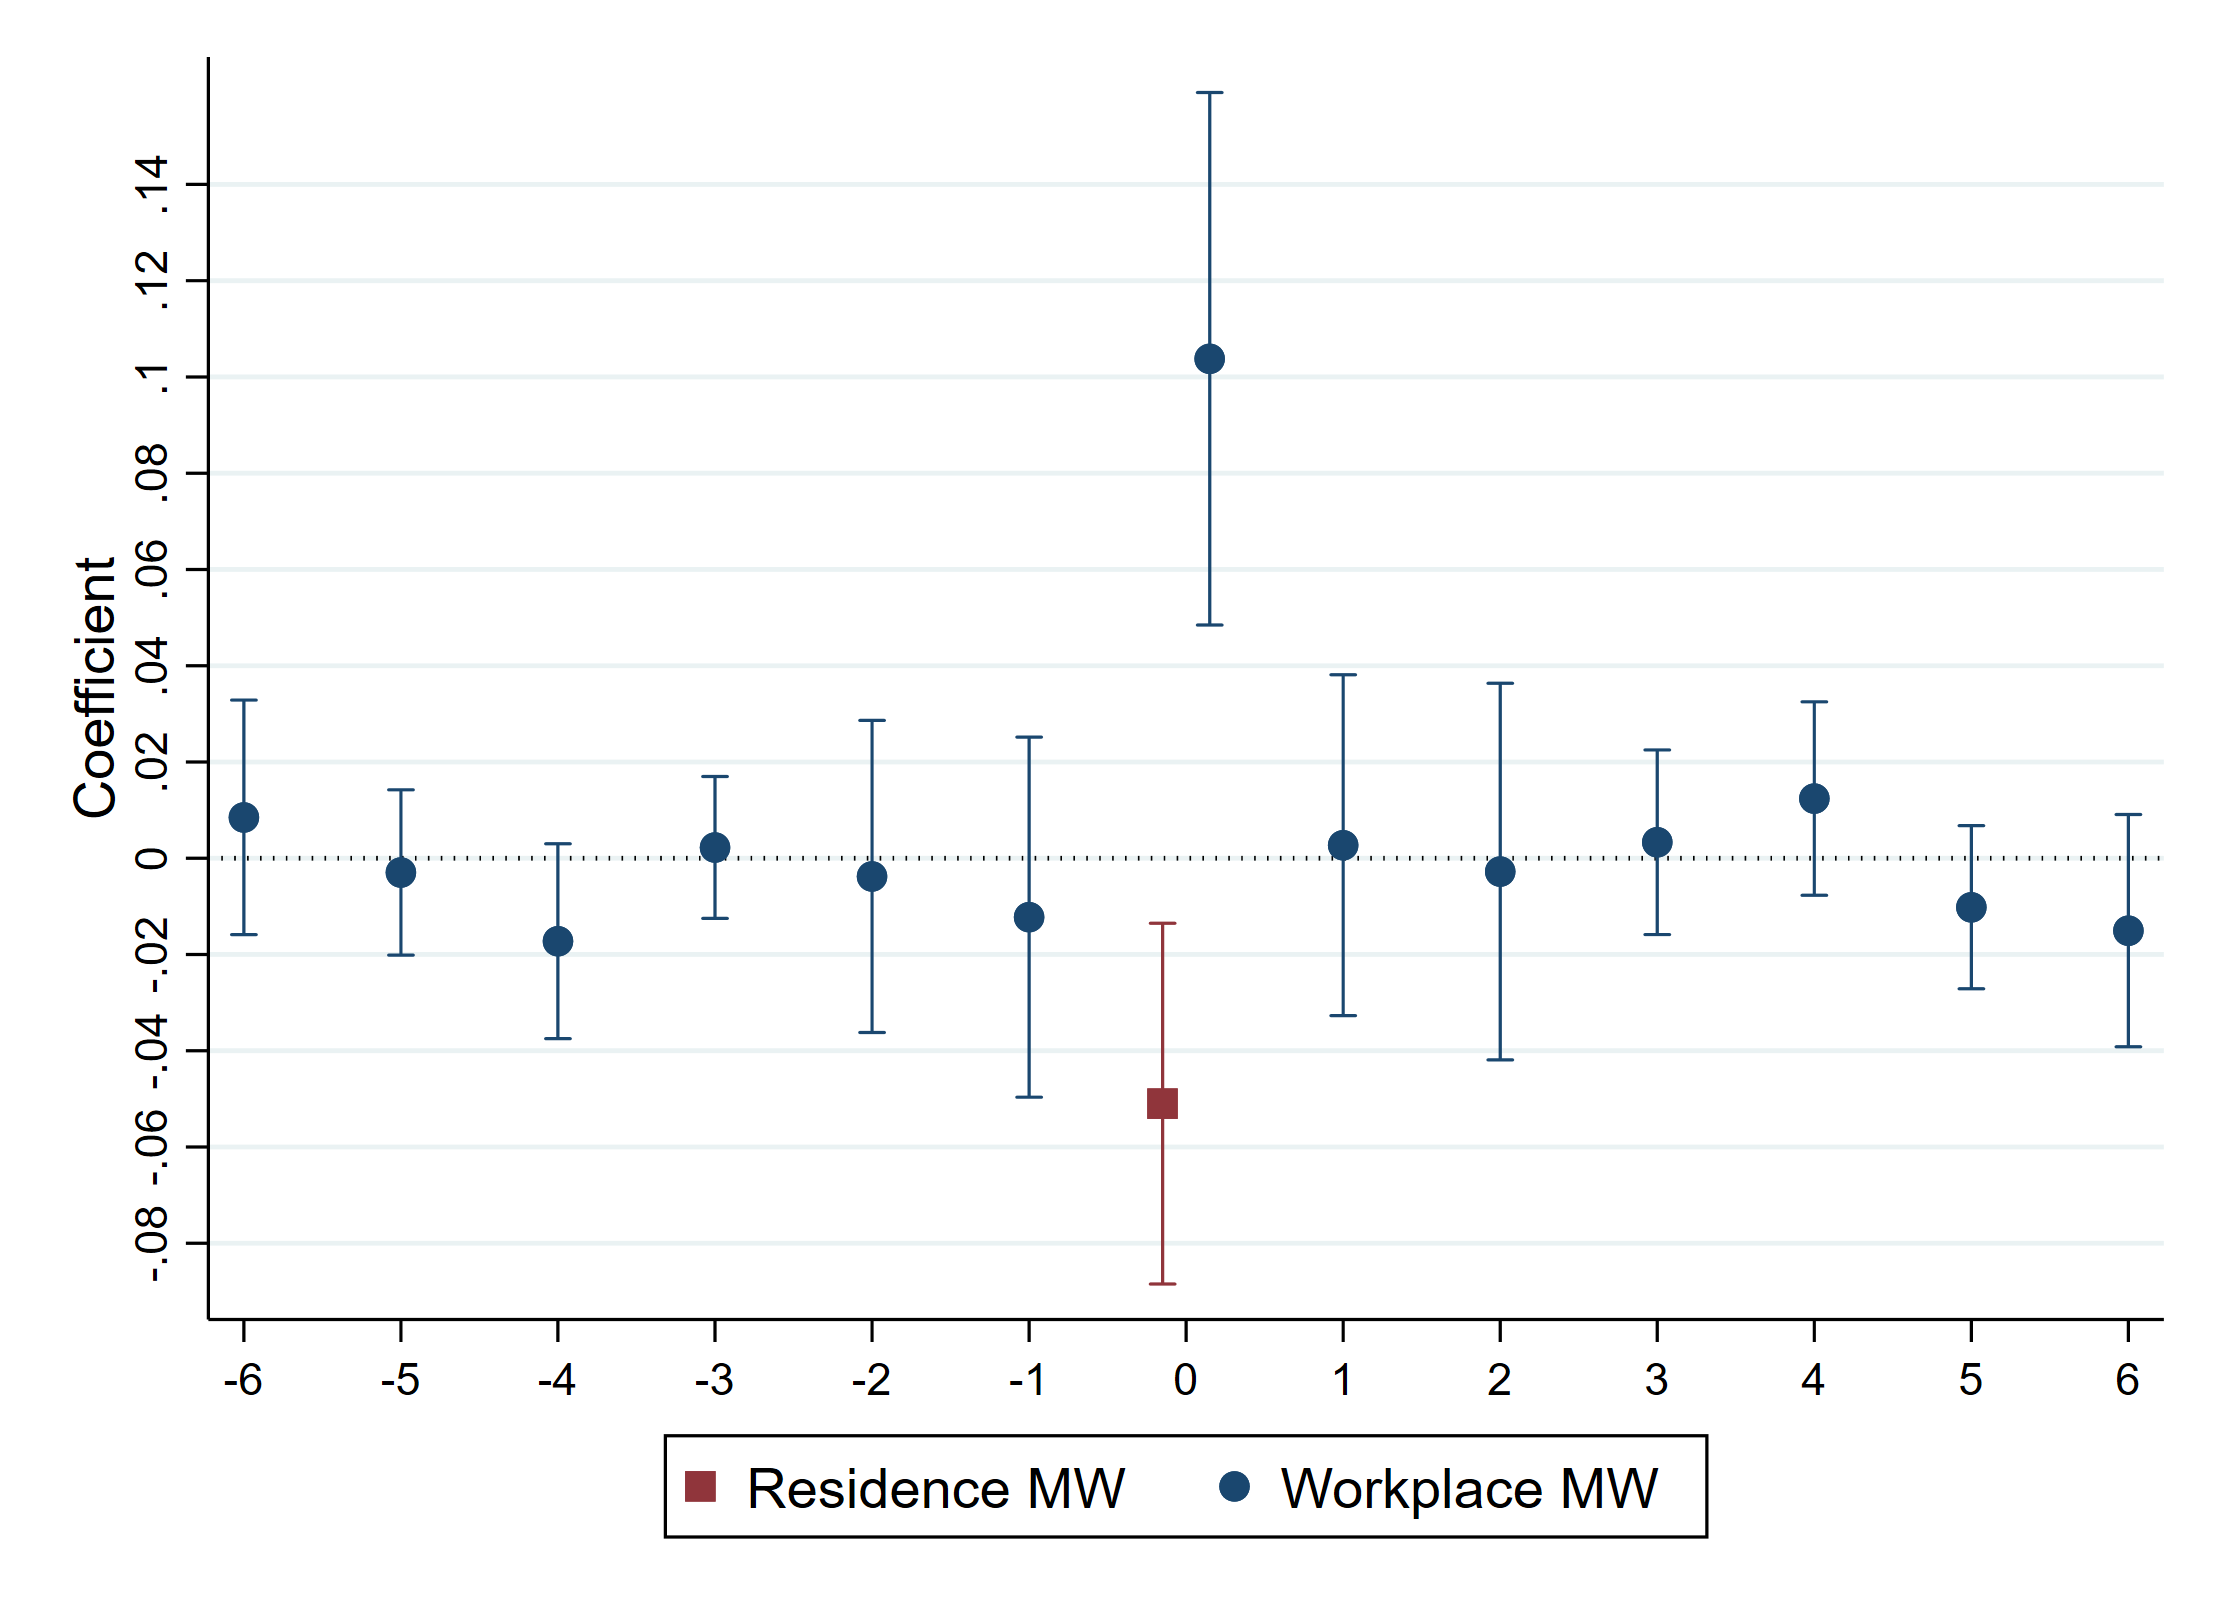
\includegraphics[width=0.68\textwidth]{../../input/fd_both_mw_wkp_only_dynamic_fullbal.png}
    \end{figure}
    
\end{frame}

\begin{frame}[label = robustness]
    \frametitle{Robustness checks and other exercises}

    Concerns about changes in migration:
    \begin{itemize} \small
        \item Literature finds small effects along several years {\small\color{gray}\parencite[e.g.,][]{PerezPerez2021}}
        \item Use different commuting shares, even allowing them to change yearly
        
        %\hyperlink{robustness_exp_mw}{\beamerbutton{Sensitivity to alternative commuting shares}}
    \end{itemize}

    \pause
    \vspace{1.5mm}
    Concerns about invalid control group:
    \begin{itemize} \small
        \item Inclusion of non-parametric CBSA trends
        \item Alternative strategies: ``stacked'' model 
        {\small \color{gray} \parencite{CegnizEtAl2019}}
    \end{itemize}

    \pause
    \vspace{1.5mm}
    Concerns that results are particular to our sample or not generalizable:
    \begin{itemize} \small
        \item Estimate on unbalanced and fully-balanced samples (instead of partially balanced)
        \item Re-weight observations to match characteristics of urban ZIP codes
    \end{itemize}
    
    \pause
    \vspace{1.5mm}
    Other exercises:
    \begin{itemize} \small
        \item Other housing categories: effects in ``Condo/cooperatives'' and ``Multifamily 5+ units''
        \item Heterogeneity based on ZIP codes that are likely to have MW \textit{residents} 
        and MW \textit{workers}
    \end{itemize}
\end{frame}

%% Main takeaway: MW levels affect rents, and their effect are determined
%%    by whether they mostly affect the MW at workplace or at residence
%%
%% Now we are going to construct an exercise to compare these rent increases
%%  with income increases, and get a sense of how much of these income accruess 
%%  to landlords

%%%%%%%%%%%%%%%%%%%%%%%%%%%%%%%%%%%%%%%%%%%%%%%%%%%%%%%%%%%%%%%%%%%%%%%%%%%%%%%%
\section{A counterfactual increase in the federal MW}

\begin{frame}
    \frametitle{Overview}
    
    Entire commuting structure determines the incidence of MW policies.
    \begin{itemize}
        \vspace{1mm}
        \item In some ZIP codes both residence and workplace MW increase
        \vspace{1mm}
        \item Other nearby ZIP codes are affected only through workplace
    \end{itemize}
    
    \pause
    \vspace{3mm}
    Consider an increase of the federal MW to \$9 in January 2020.
    \begin{itemize}
        \vspace{1mm}
        \item Changes nominal income $\{\Delta Y_i\}$ and housing expenditure $\{\Delta H_i R_i\}$
    \end{itemize}
    
    \vspace{2mm}
    How much out of each extra dollar is captured by landlords?
    \pause 

    \vspace{2mm}
    Define the \textit{share pocketed} as 
    \begin{equation*}
        \rho_i := \frac{\Delta H_i R_i}{\Delta Y_i} =  \frac{H^{\post}_i R^{\post}_i - H^{\pre}_i R^{\pre}_i}{\Delta Y_i}
    \end{equation*}
    where ``Pre'' and ``Post'' indicate moments before and after the increase.
   
\end{frame}

\begin{frame}[label = share_pocketed_model]
    \frametitle{Share pocketed under the model}

    According to the model,
    $$
    \Delta r_i = \beta \Delta {\color{blue}\mw_i^{\wkp}} + \gamma \Delta {\color{red}\mw_i^{\res}}
    $$
    We also define, for $y_i = \ln Y_i$,
    $$
    \Delta y_i = \varepsilon \Delta {\color{blue}\mw_i^{\wkp}}
    $$
    We estimate $\varepsilon$ using IRS data. \hyperlink{wages_results}{\beamerbutton{Estimation results}}

    \pause
    \vspace{3mm}
    Assuming $H^{\pre}_i = H^{\post}_i = H_i$, the share pocketed becomes
    \begin{equation*}
        \rho_i = \alpha_i \left[
                  \frac{\exp \left( \beta \Delta {\color{blue}\mw_i^{\wkp}} 
                                 + \gamma \Delta {\color{red}\mw_i^{\res}} \right) - 1 }
                       {\exp \left( \varepsilon \Delta {\color{blue}\mw_i^{\wkp}}  \right) - 1 }
                         \right]
    \end{equation*}
    where $\alpha_i = H_i R_i / Y_i$ is the share of $i$'s expenditure in housing. Assume $\alpha_i = \alpha$ for all $i$.
    
    \pause
    \vspace{3mm}
    Use estimates to compute $\{\rho_i\}$ for urban ZIP codes located in affected CBSAs.
\end{frame}

\begin{frame}
    \frametitle{The distribution of the share pocketed by landlords}
    
    \vspace{1mm}
    \begin{figure}
        \centering
        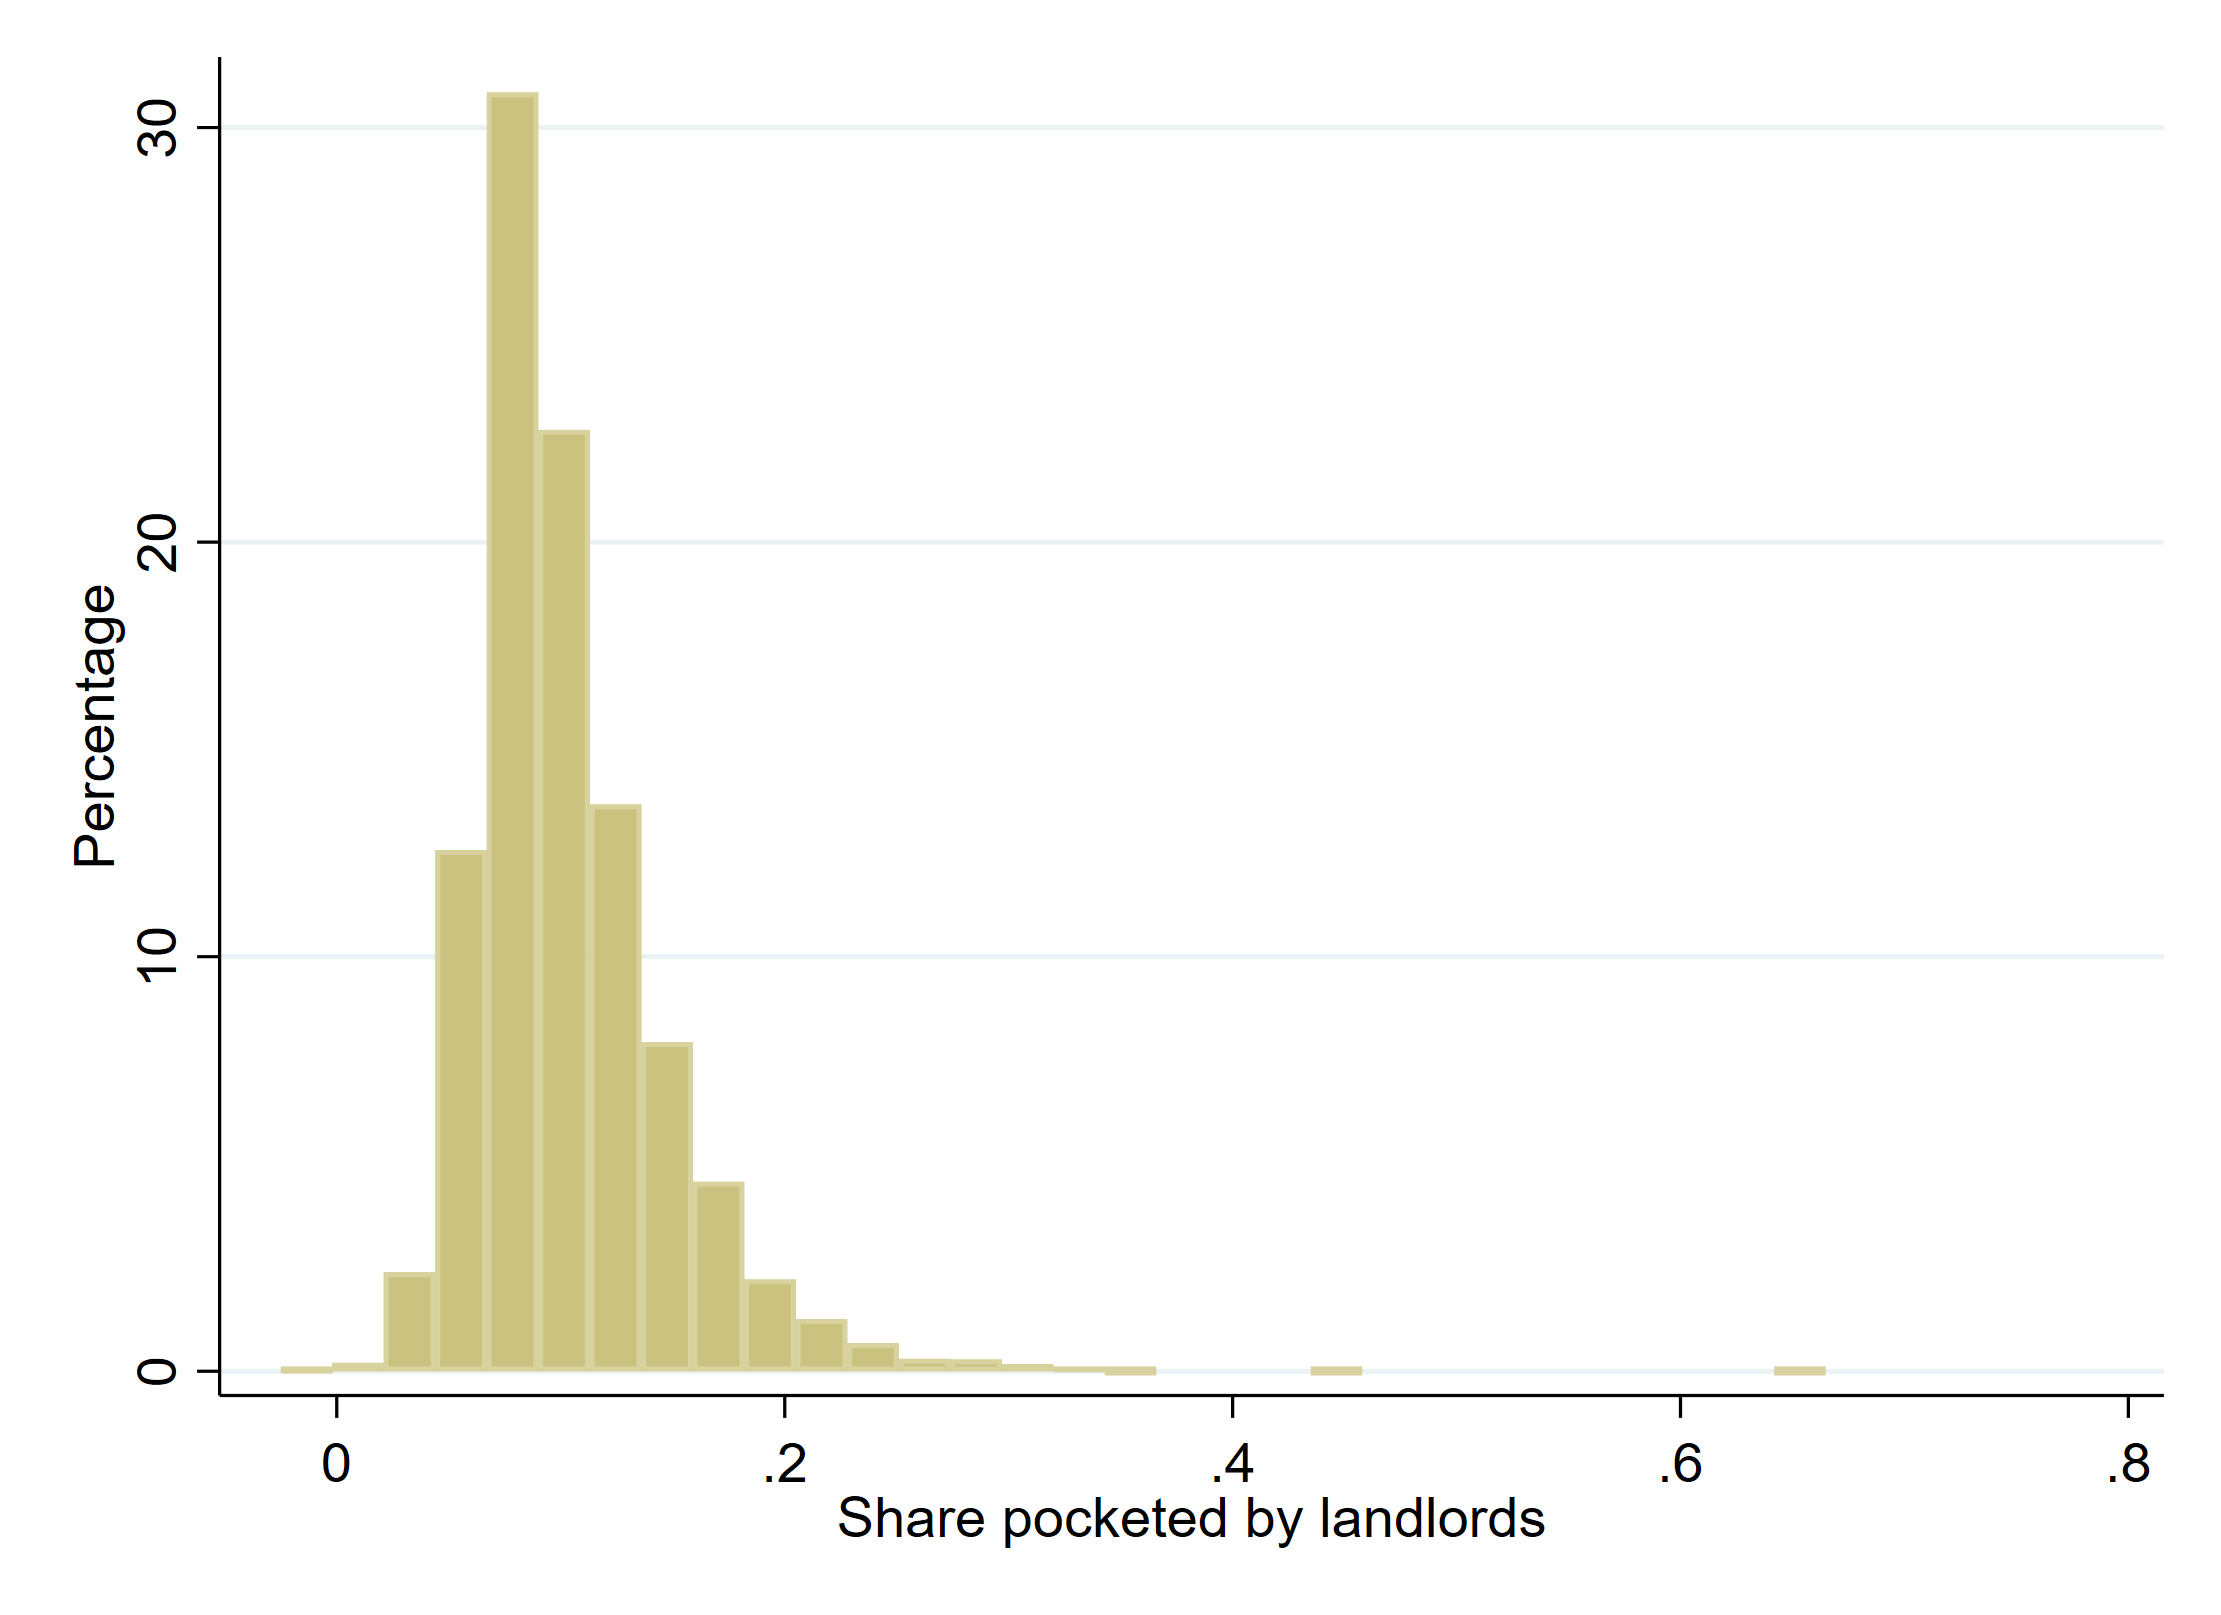
\includegraphics[width = 0.62\textwidth]{counterfactuals/output/hist_rho.png}
    \end{figure}   

    \vspace{-1mm}
    \scriptsize
    Notes: Share estimated using parameters $\beta = 0.0546$, $\gamma = -0.0207$, $\varepsilon = 0.1083$, and $\alpha=0.35$.
    We include 6,952 ZIP codes located in CBSAs where the average estimated income increase
    is of at least 0.1\%. 
    The residence MW did not change for 1,070 ZIP codes in this sample.
\end{frame}

\begin{frame}[label=share_pocketed]
    \frametitle{Share pocketed in Chicago CBSA}

    \begin{columns}
        \begin{column}{0.45\textwidth}

            Share pocketed is larger inside of Cook County.

            \vspace{3mm}
            Mapping intermediate computations:
            \begin{itemize}
                \item Estimated changes in MW measures \hyperlink{changes_mw_measures}{\beamerbutton{here}}
                \item Estimated changes in rents and income \hyperlink{changes_rents_inc}{\beamerbutton{here}}
            \end{itemize}
                        
        \end{column}
        \begin{column}{0.55\textwidth}
            \vspace{-16mm}
            \begin{figure}
                \centering
                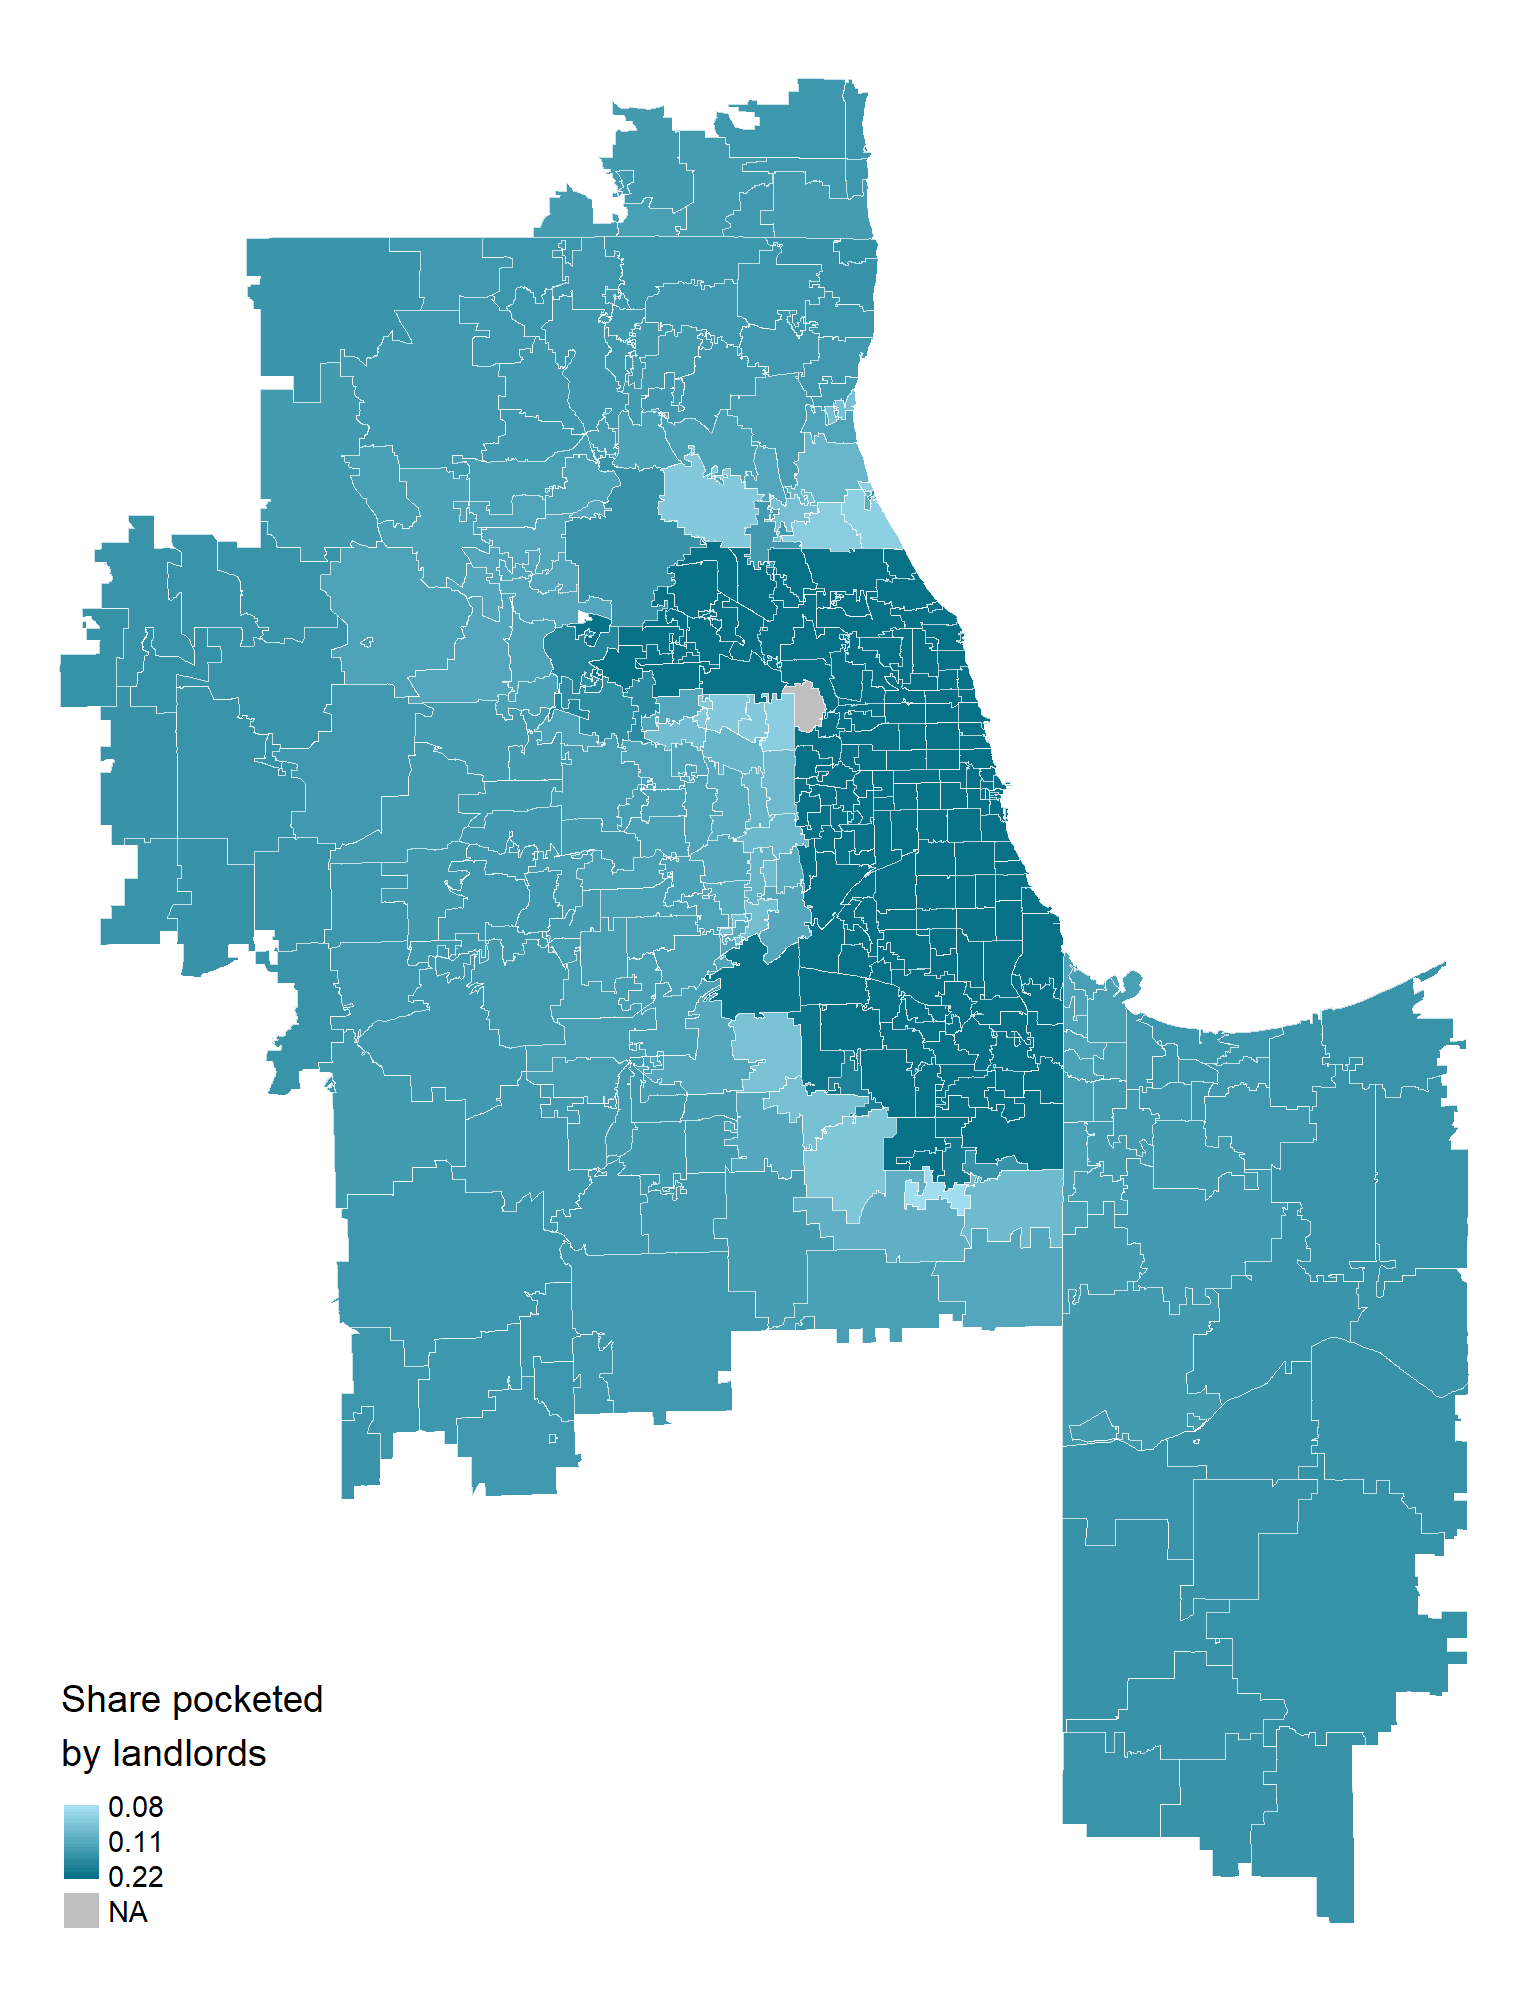
\includegraphics[width = 0.87\textwidth]{counterfactuals/output/chicago_rho.png}
            \end{figure}   
        \end{column}
    \end{columns}
    
\end{frame}

% \begin{frame}
%     \frametitle{The incidence of MW changes according to intensity of treatment}
    
%     \begin{figure}
%         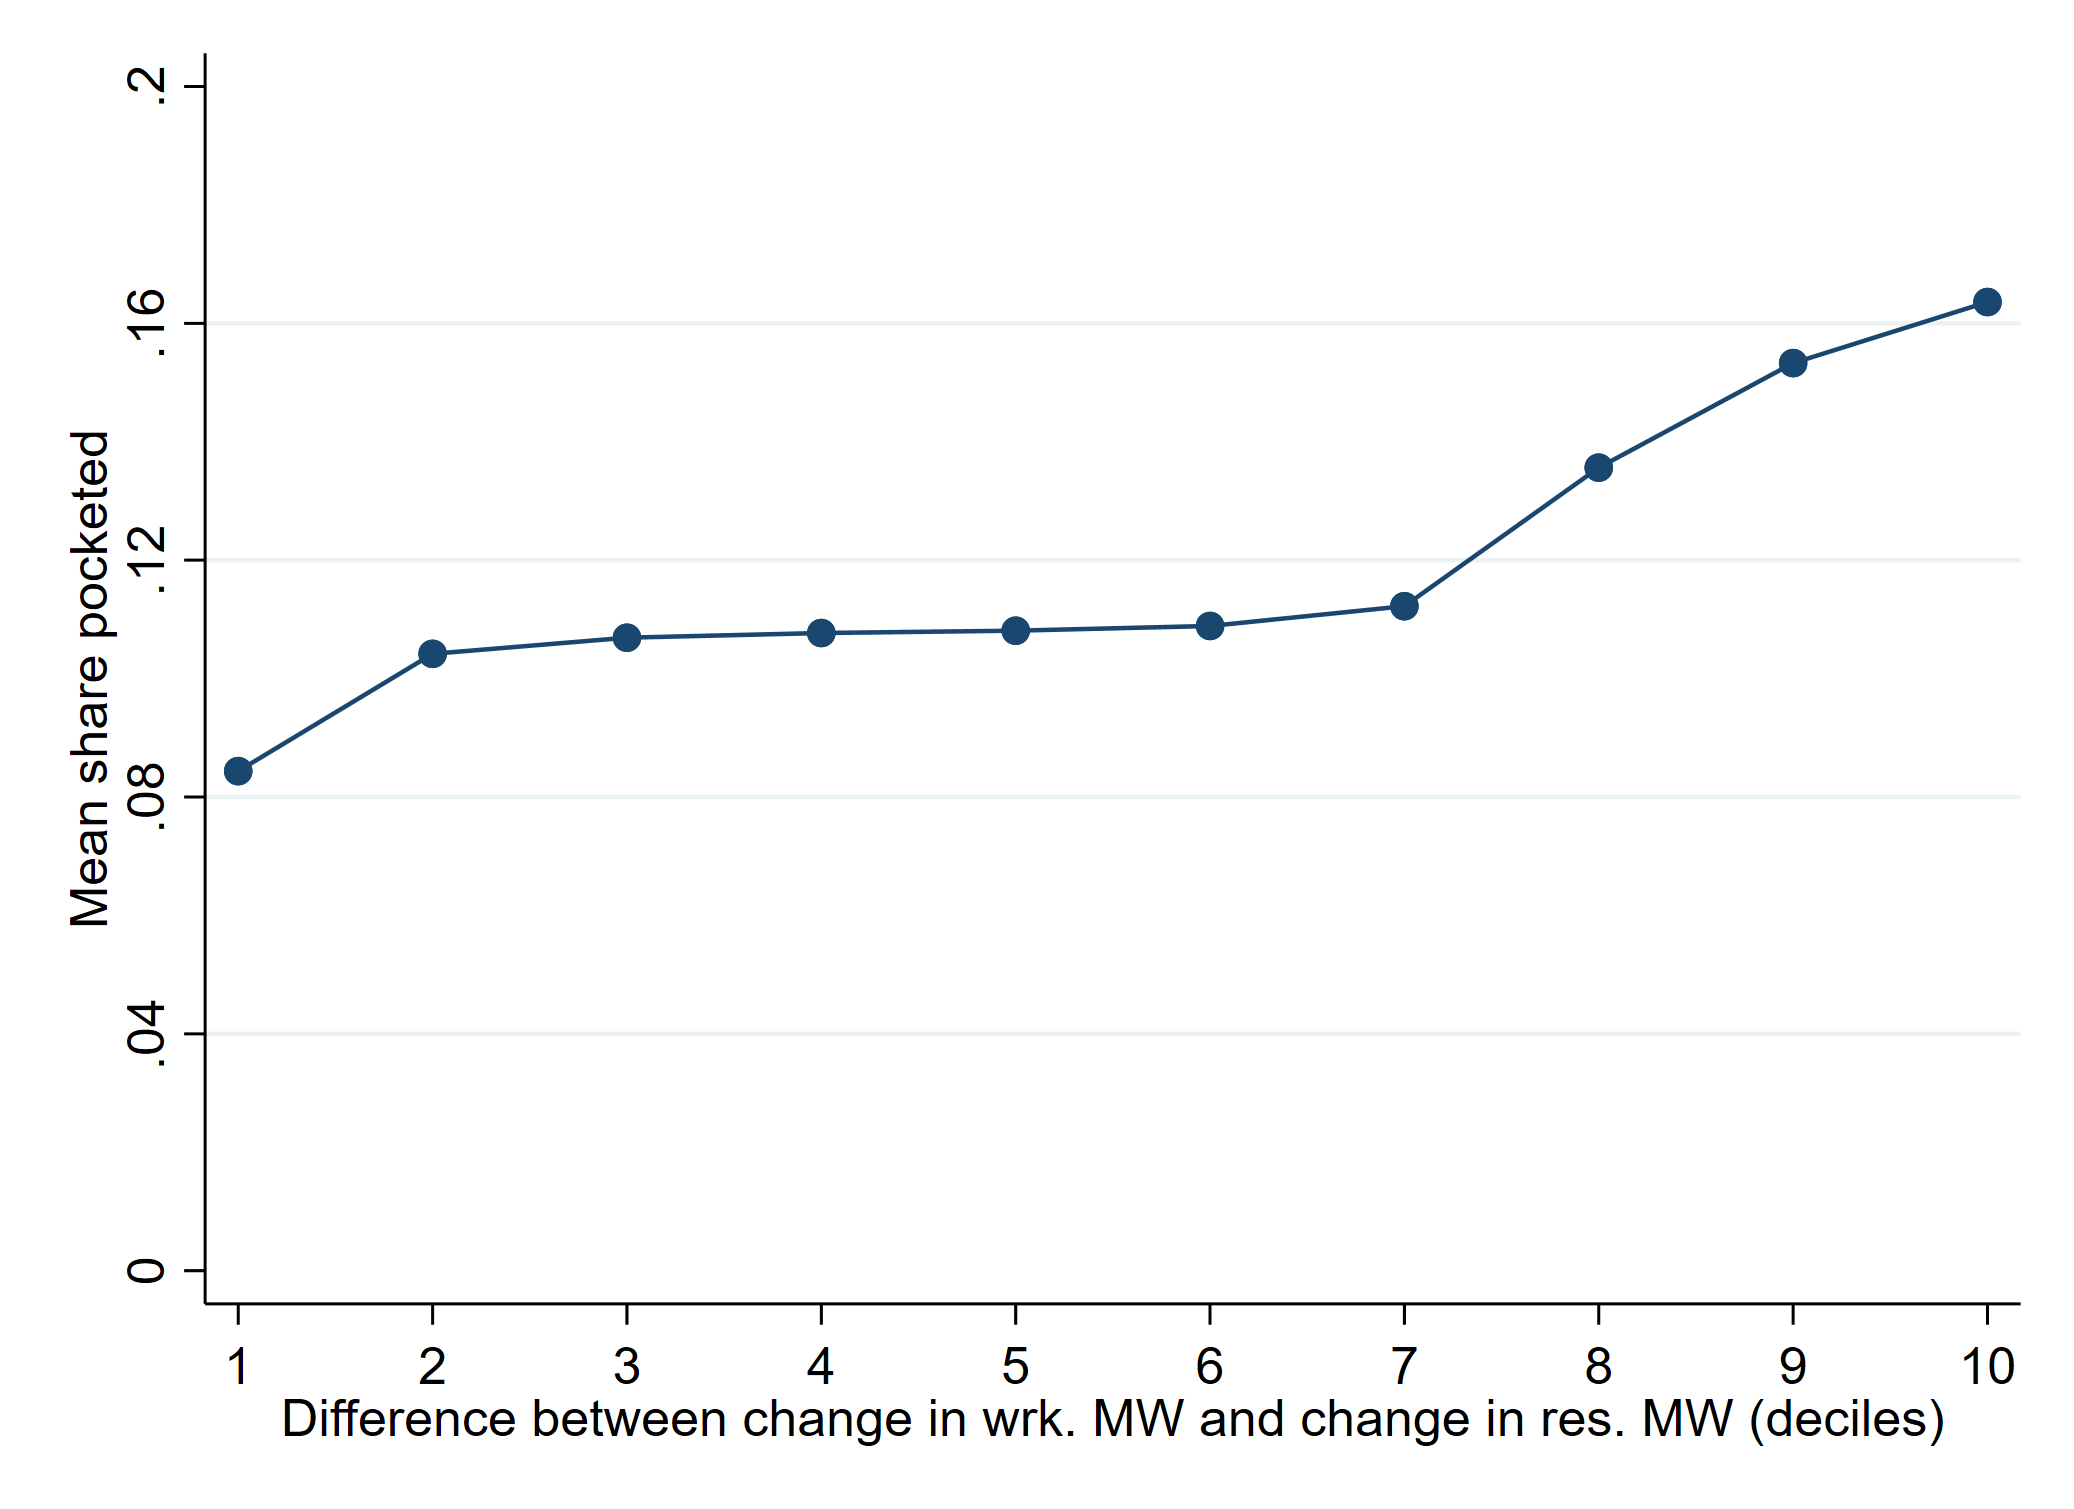
\includegraphics[width = 0.62\textwidth]{counterfactuals/output/deciles_diff.png}
%     \end{figure}

%     \vspace{-1mm}
%     \scriptsize
%     Notes: Share estimated using parameters $\beta = 0.0546$, $\gamma = -0.0207$, $\varepsilon = 0.1083$, and $\alpha=0.35$.
%     We include 6,952 ZIP codes located in CBSAs where average estimated income increase
%     is of at least 0.1\%. 
% \end{frame}

%%%%%%%%%%%%%%%%%%%%%%%%%%%%%%%%%%%%%%%%%%%%%%%%%%%%%%%%%%%%%%%%%%%%%%%%%%%%%%%%
\section{Concluding remarks}

\begin{frame}
    \frametitle{Conclusions}
    
    \begin{itemize}
        \item When studying effects of place-based policies on housing markets one 
        must account for divergence between workplace and residence locations
        \vspace{2mm}
        \item In the case of the MW, hikes in workplace locations \textit{increase} rents
        whereas hikes in residence locations \textit{decrease} rents
        \vspace{2mm}
        \item Even with a two-parameter model we are able to describe and predict 
        rich spatial patterns in rent changes
        \vspace{2mm}
        \item Landlords pocket a non-negligible fraction of the income increase 
        generated by the MW
        \vspace{2mm}
        \item Ignoring the housing market will lead to an overstatement of the positive
        effects of MW policies
    \end{itemize}
    
\end{frame}

\begin{frame}[c]
    \Large Thank You!

    \vspace{3mm}
    \normalsize E-mail: \texttt{\url{santiago_hermo@brown.edu}}

    \vspace{2mm}
    \normalsize Draft: \texttt{\url{bit.ly/min_wage_rent}}
\end{frame}

%%%%%%%%%%%%%%%%%%%%%%%%%%%%%%%%%%%%%%%%%%%%%%%%%%%%%%%%%%%%%%%%%%%%%%%%%%%%%%%%%%%%%%%%%%
%                                       APPENDIX                                        %
%%%%%%%%%%%%%%%%%%%%%%%%%%%%%%%%%%%%%%%%%%%%%%%%%%%%%%%%%%%%%%%%%%%%%%%%%%%%%%%%%%%%%%%%%%

\appendix

\renewcommand\thetable{\thesection.\arabic{table}}
\renewcommand\thefigure{\thesection.\arabic{figure}} 
\setcounter{table}{0}
\setcounter{figure}{0}

\section{Appendix}

\begin{frame}[label = nyc_example]
\frametitle{New York (MW changes in January 2019)}
    \begin{columns}
        \begin{column}{0.50\textwidth}
            \vspace{-4mm}
            \begin{figure}
                \centering
                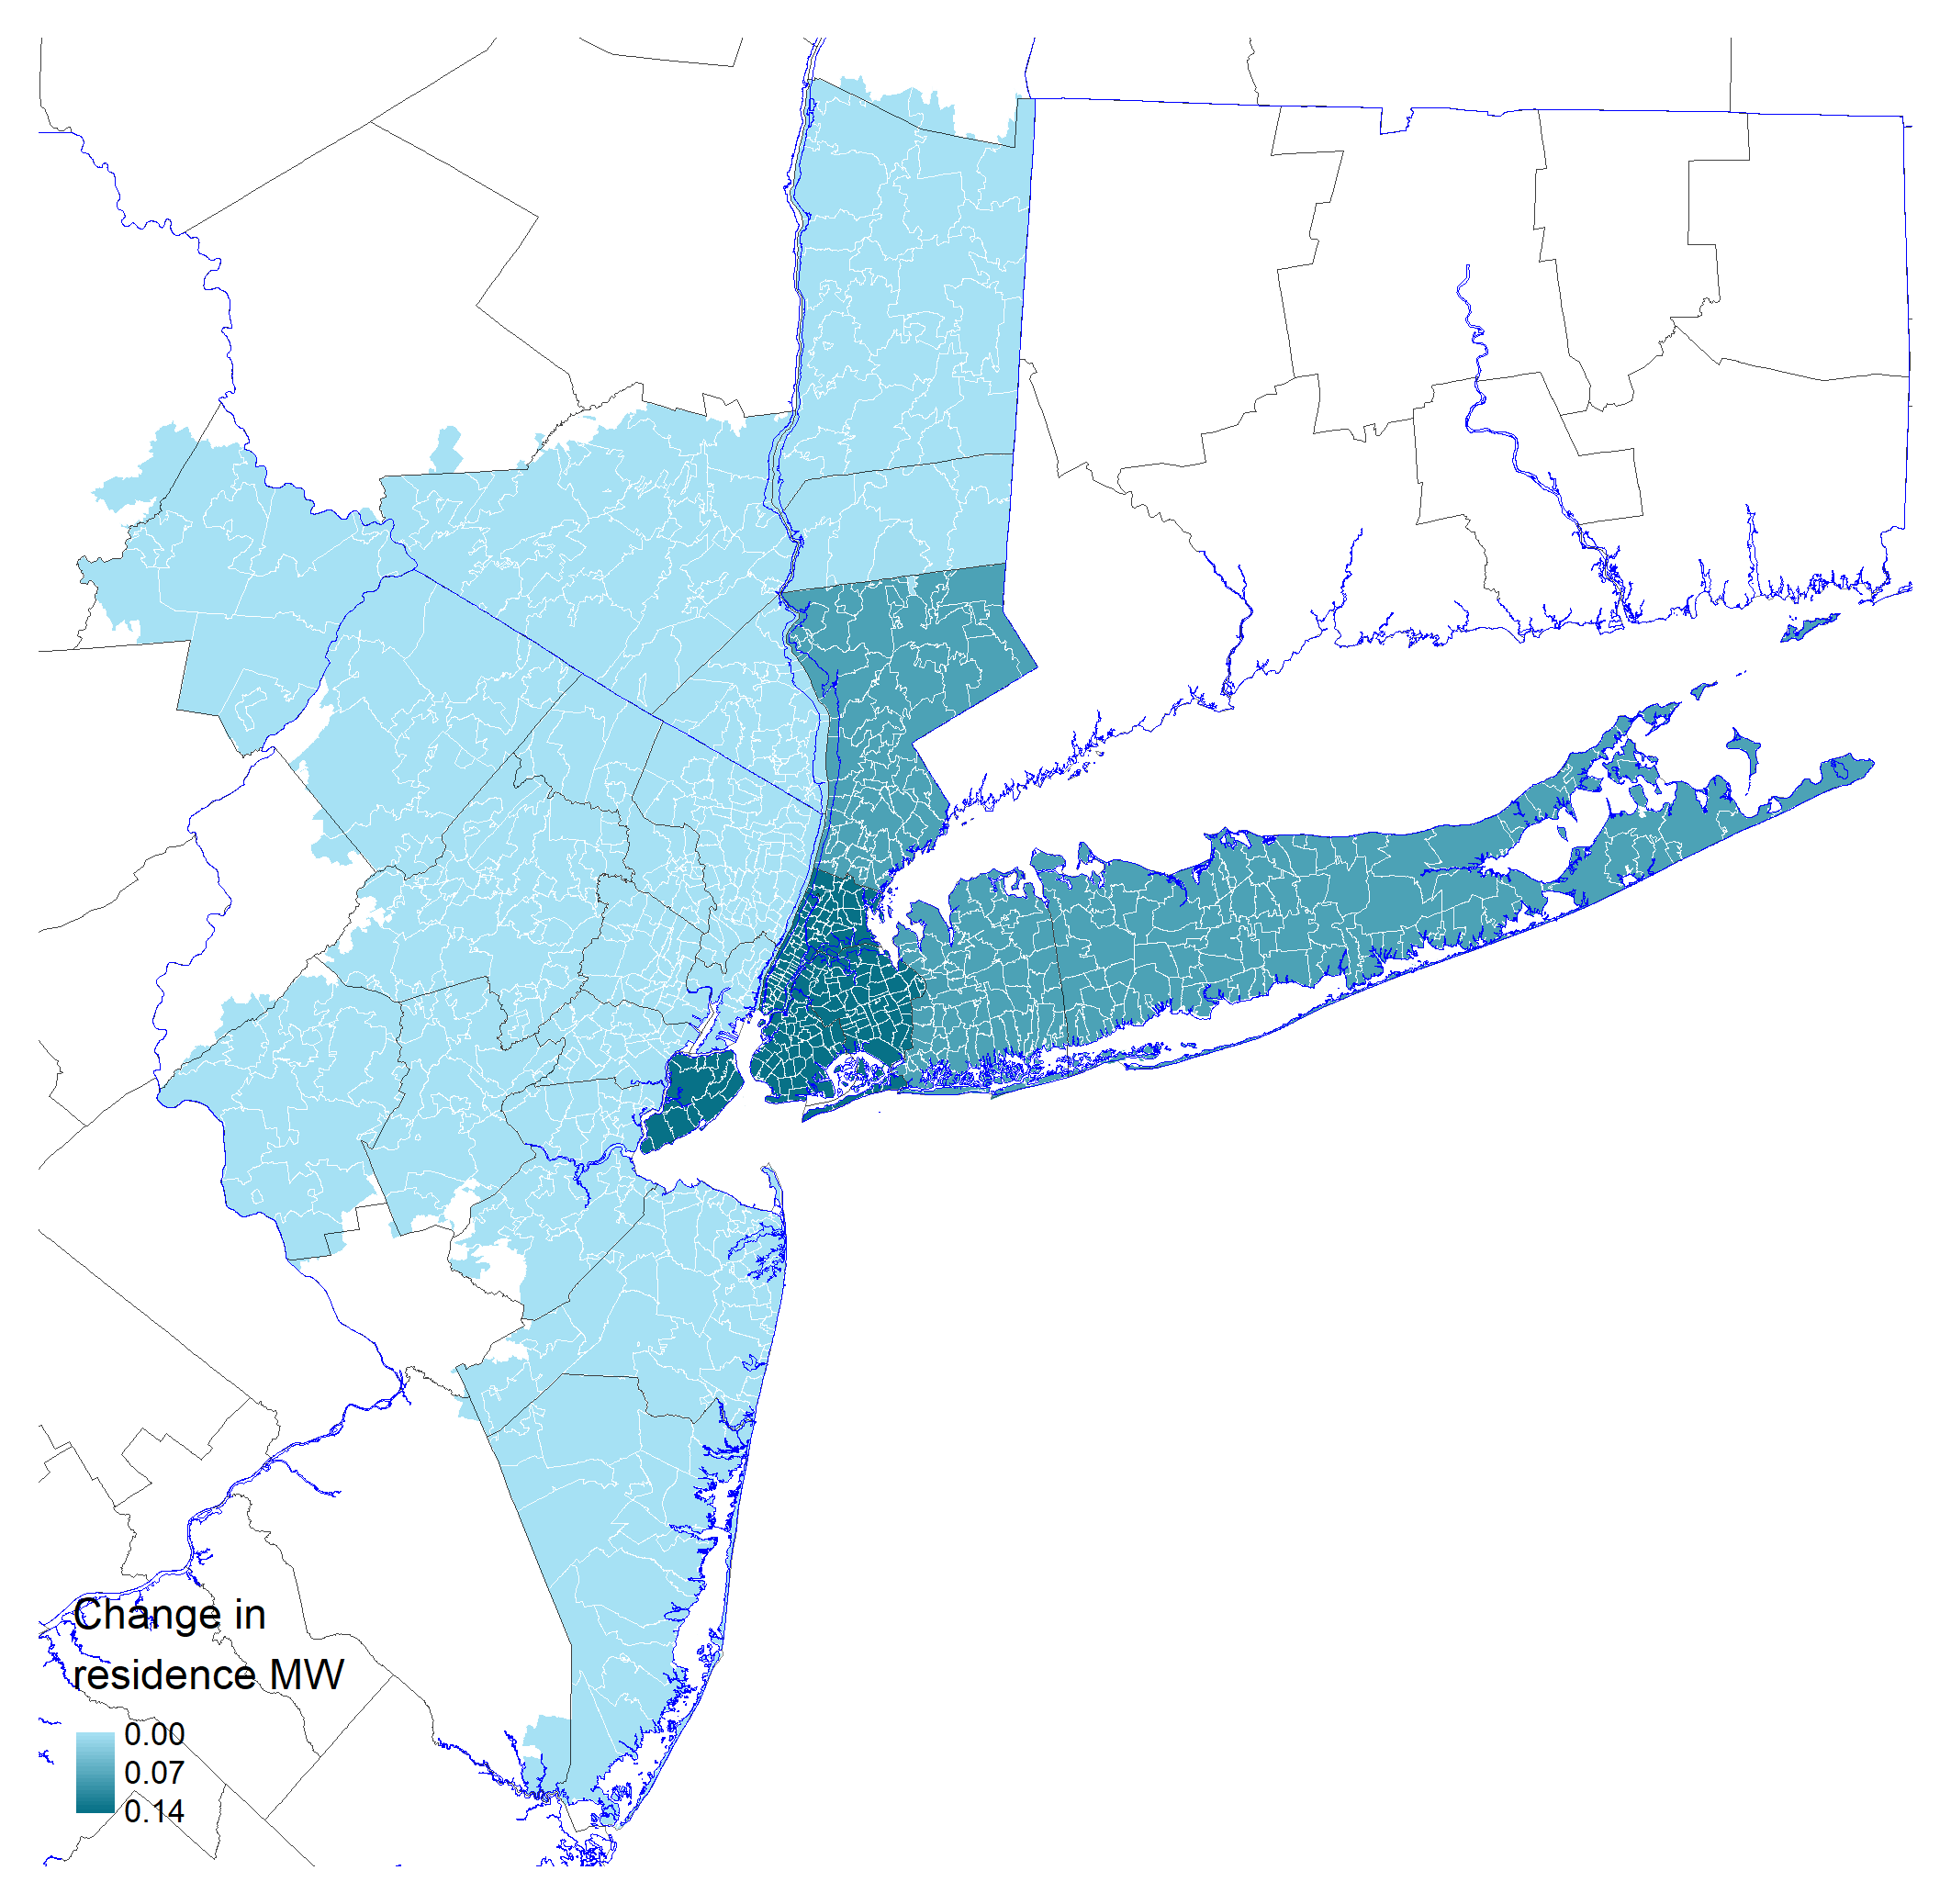
\includegraphics[scale = 0.36]{maps_events/output/nyc_2018-12_statutory_mw.png}
            \end{figure}   
        \end{column}
        \begin{column}{0.50\textwidth}
            \vspace{-4mm}
            \begin{figure}
                \centering
                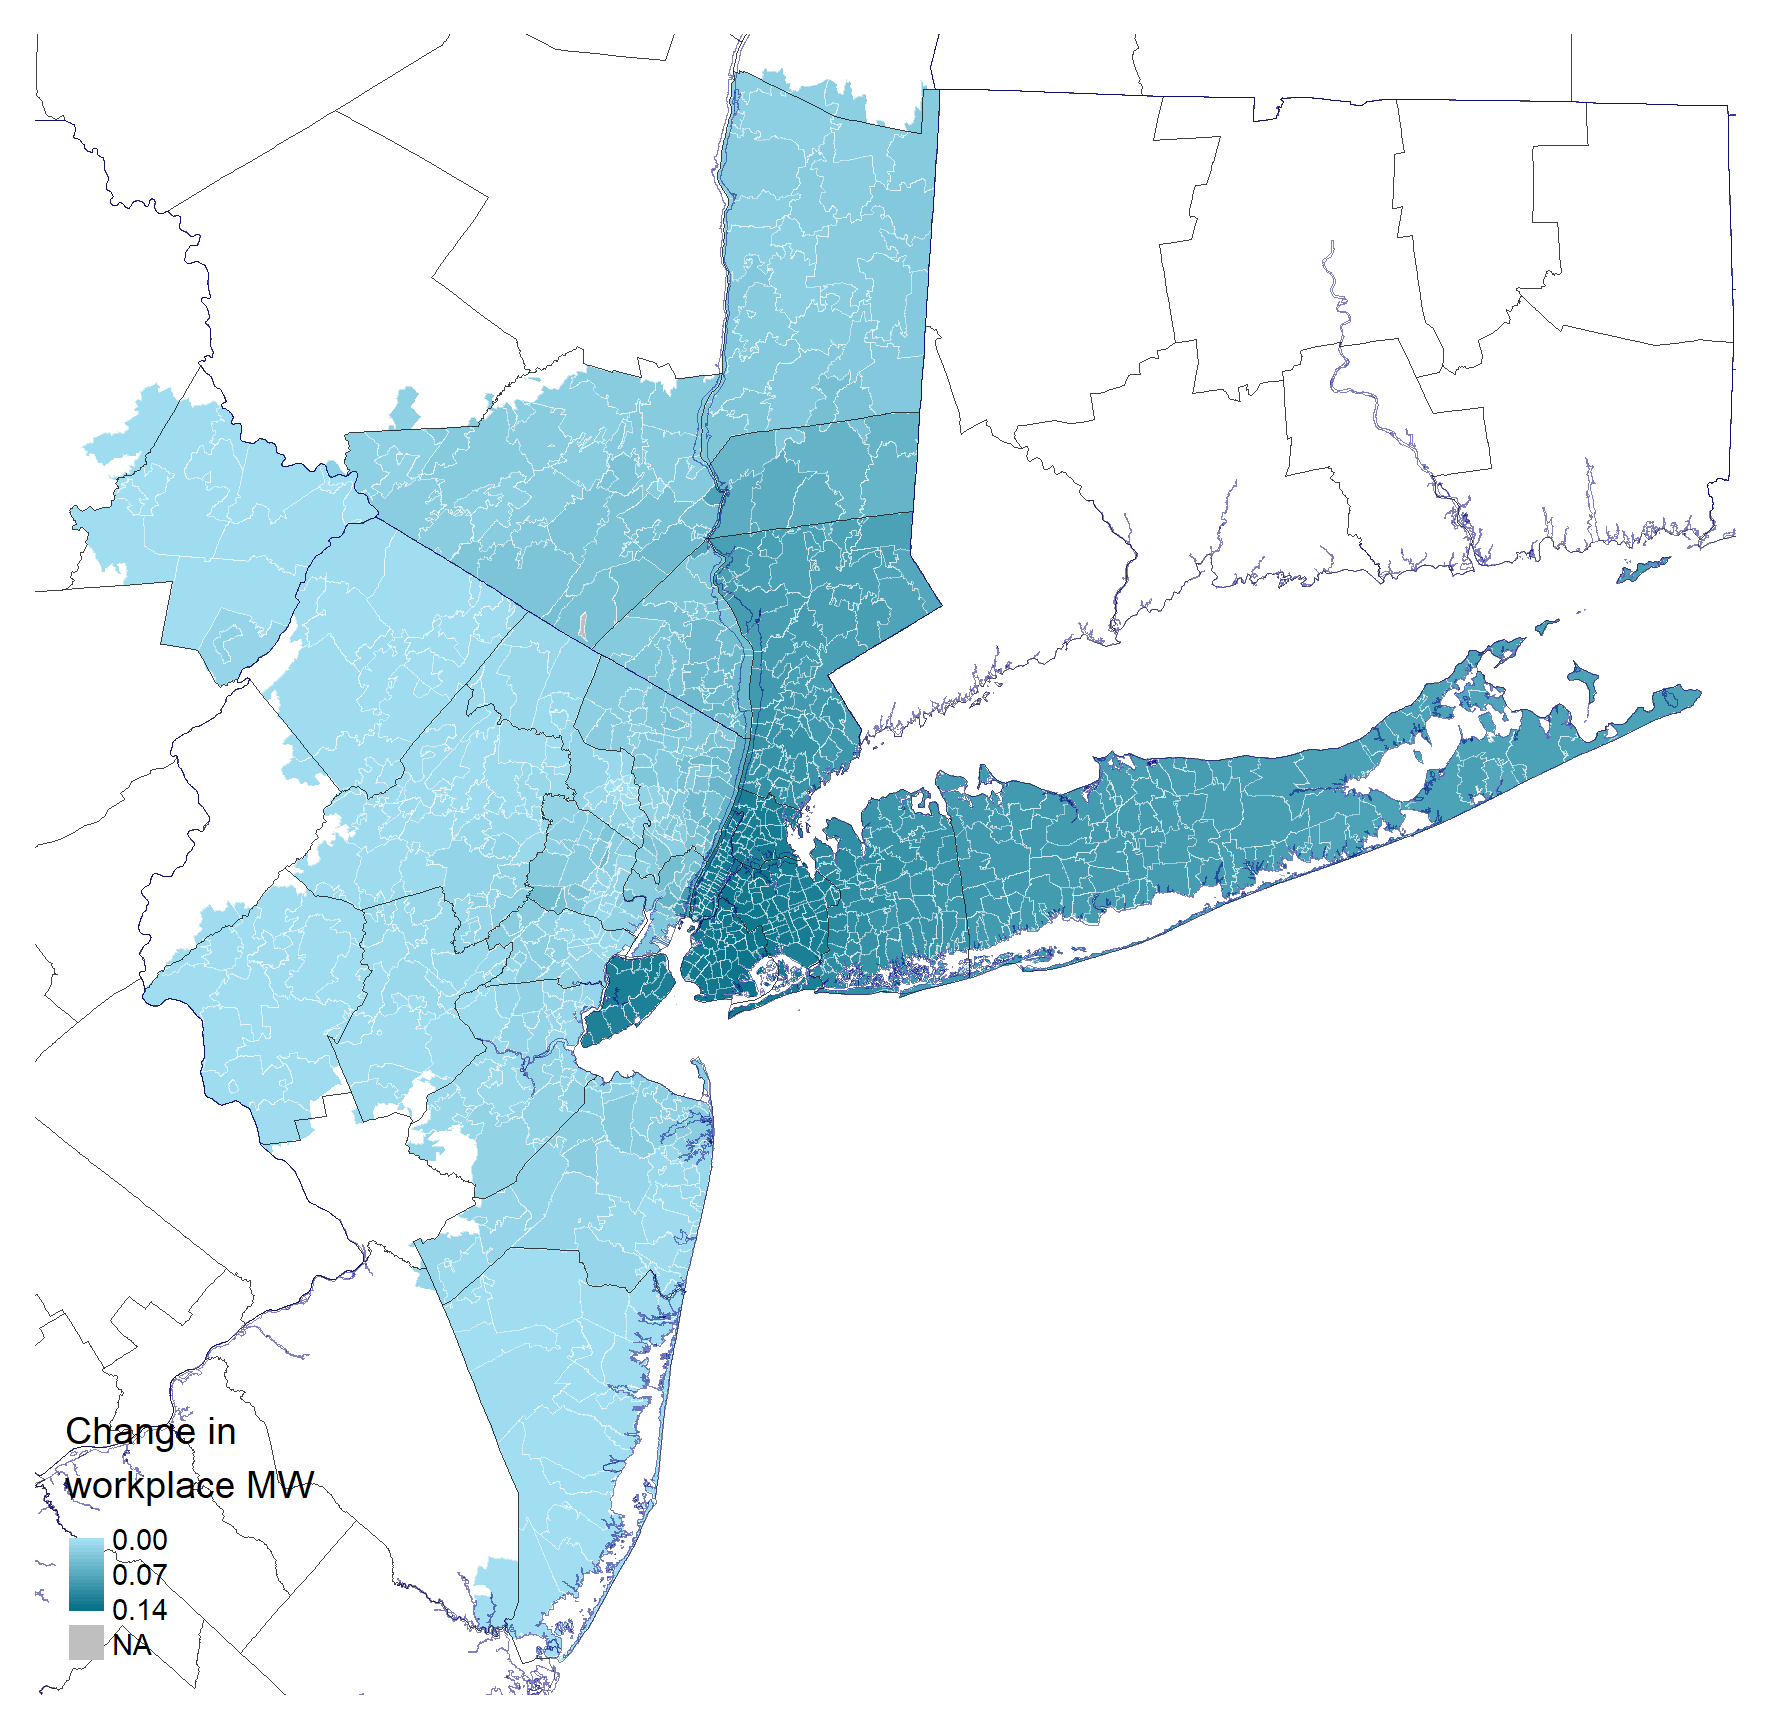
\includegraphics[scale = 0.36]{maps_events/output/nyc2018-12_wkp_mw.png}
            \end{figure}   
        \end{column}
    \end{columns}
    \hyperlink{chi_example}{\beamerbutton{Go back}}
\end{frame}

\begin{frame}[label = bay_example]
\frametitle{Bay area (MW changes in January 2019)}
    \begin{columns}
        \begin{column}{0.50\textwidth}
            \vspace{-4mm}
            \begin{figure}
                \centering
                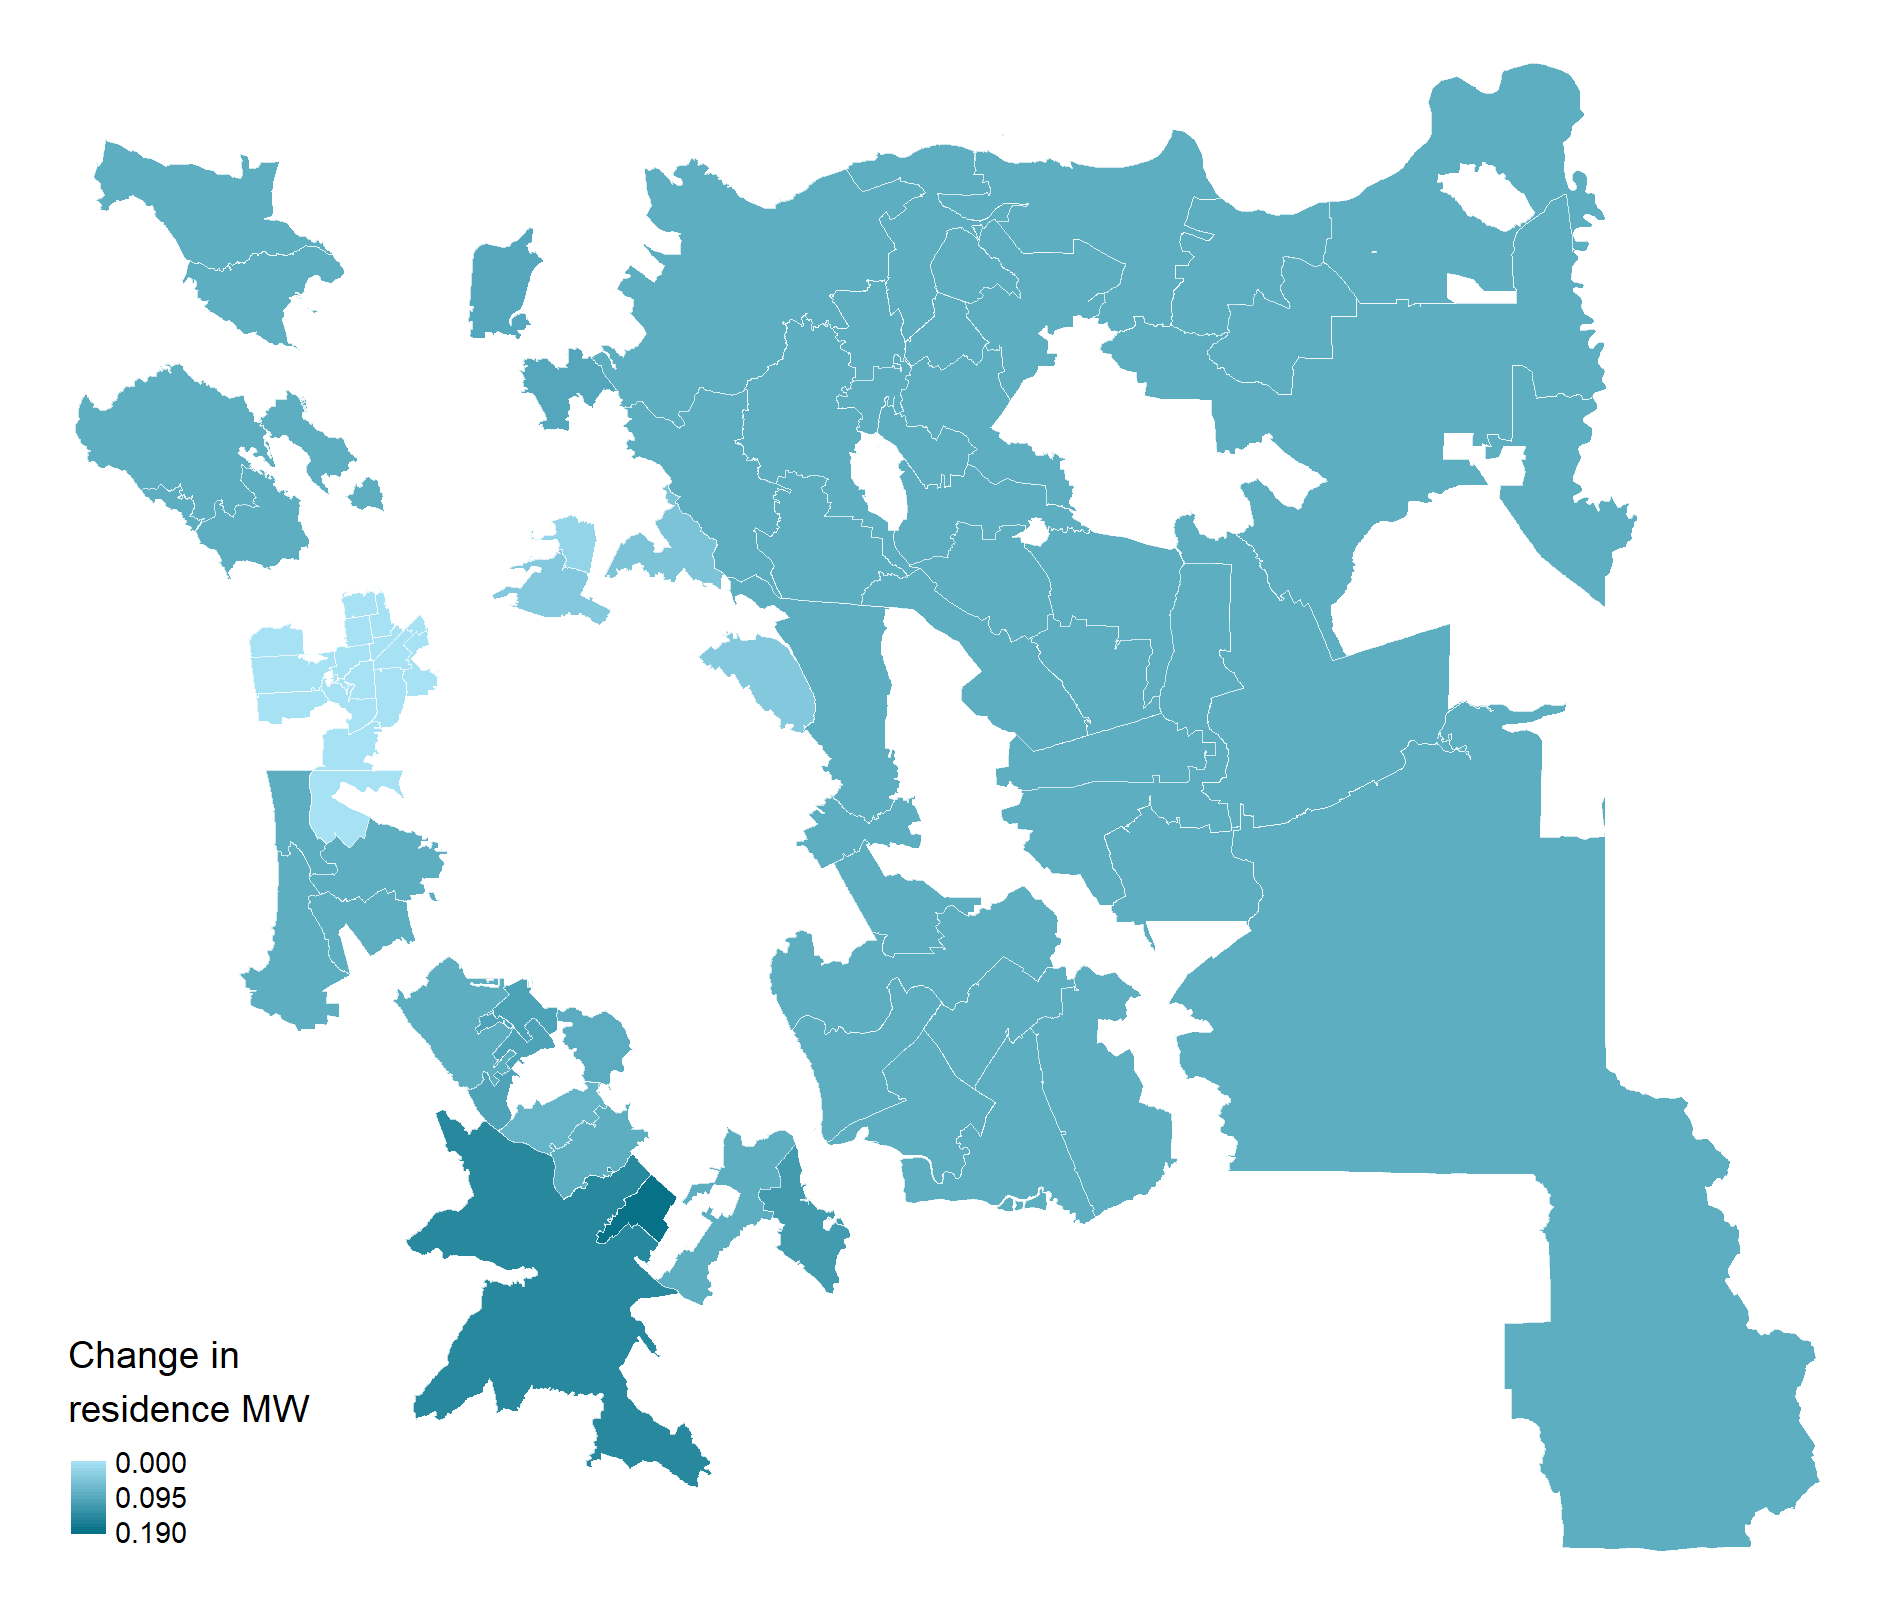
\includegraphics[scale = 0.36]{maps_events/output/bay_area_2018-12_statutory_mw.png}
            \end{figure}   
        \end{column}
        \begin{column}{0.50\textwidth}
            \vspace{-4mm}
            \begin{figure}
                \centering
                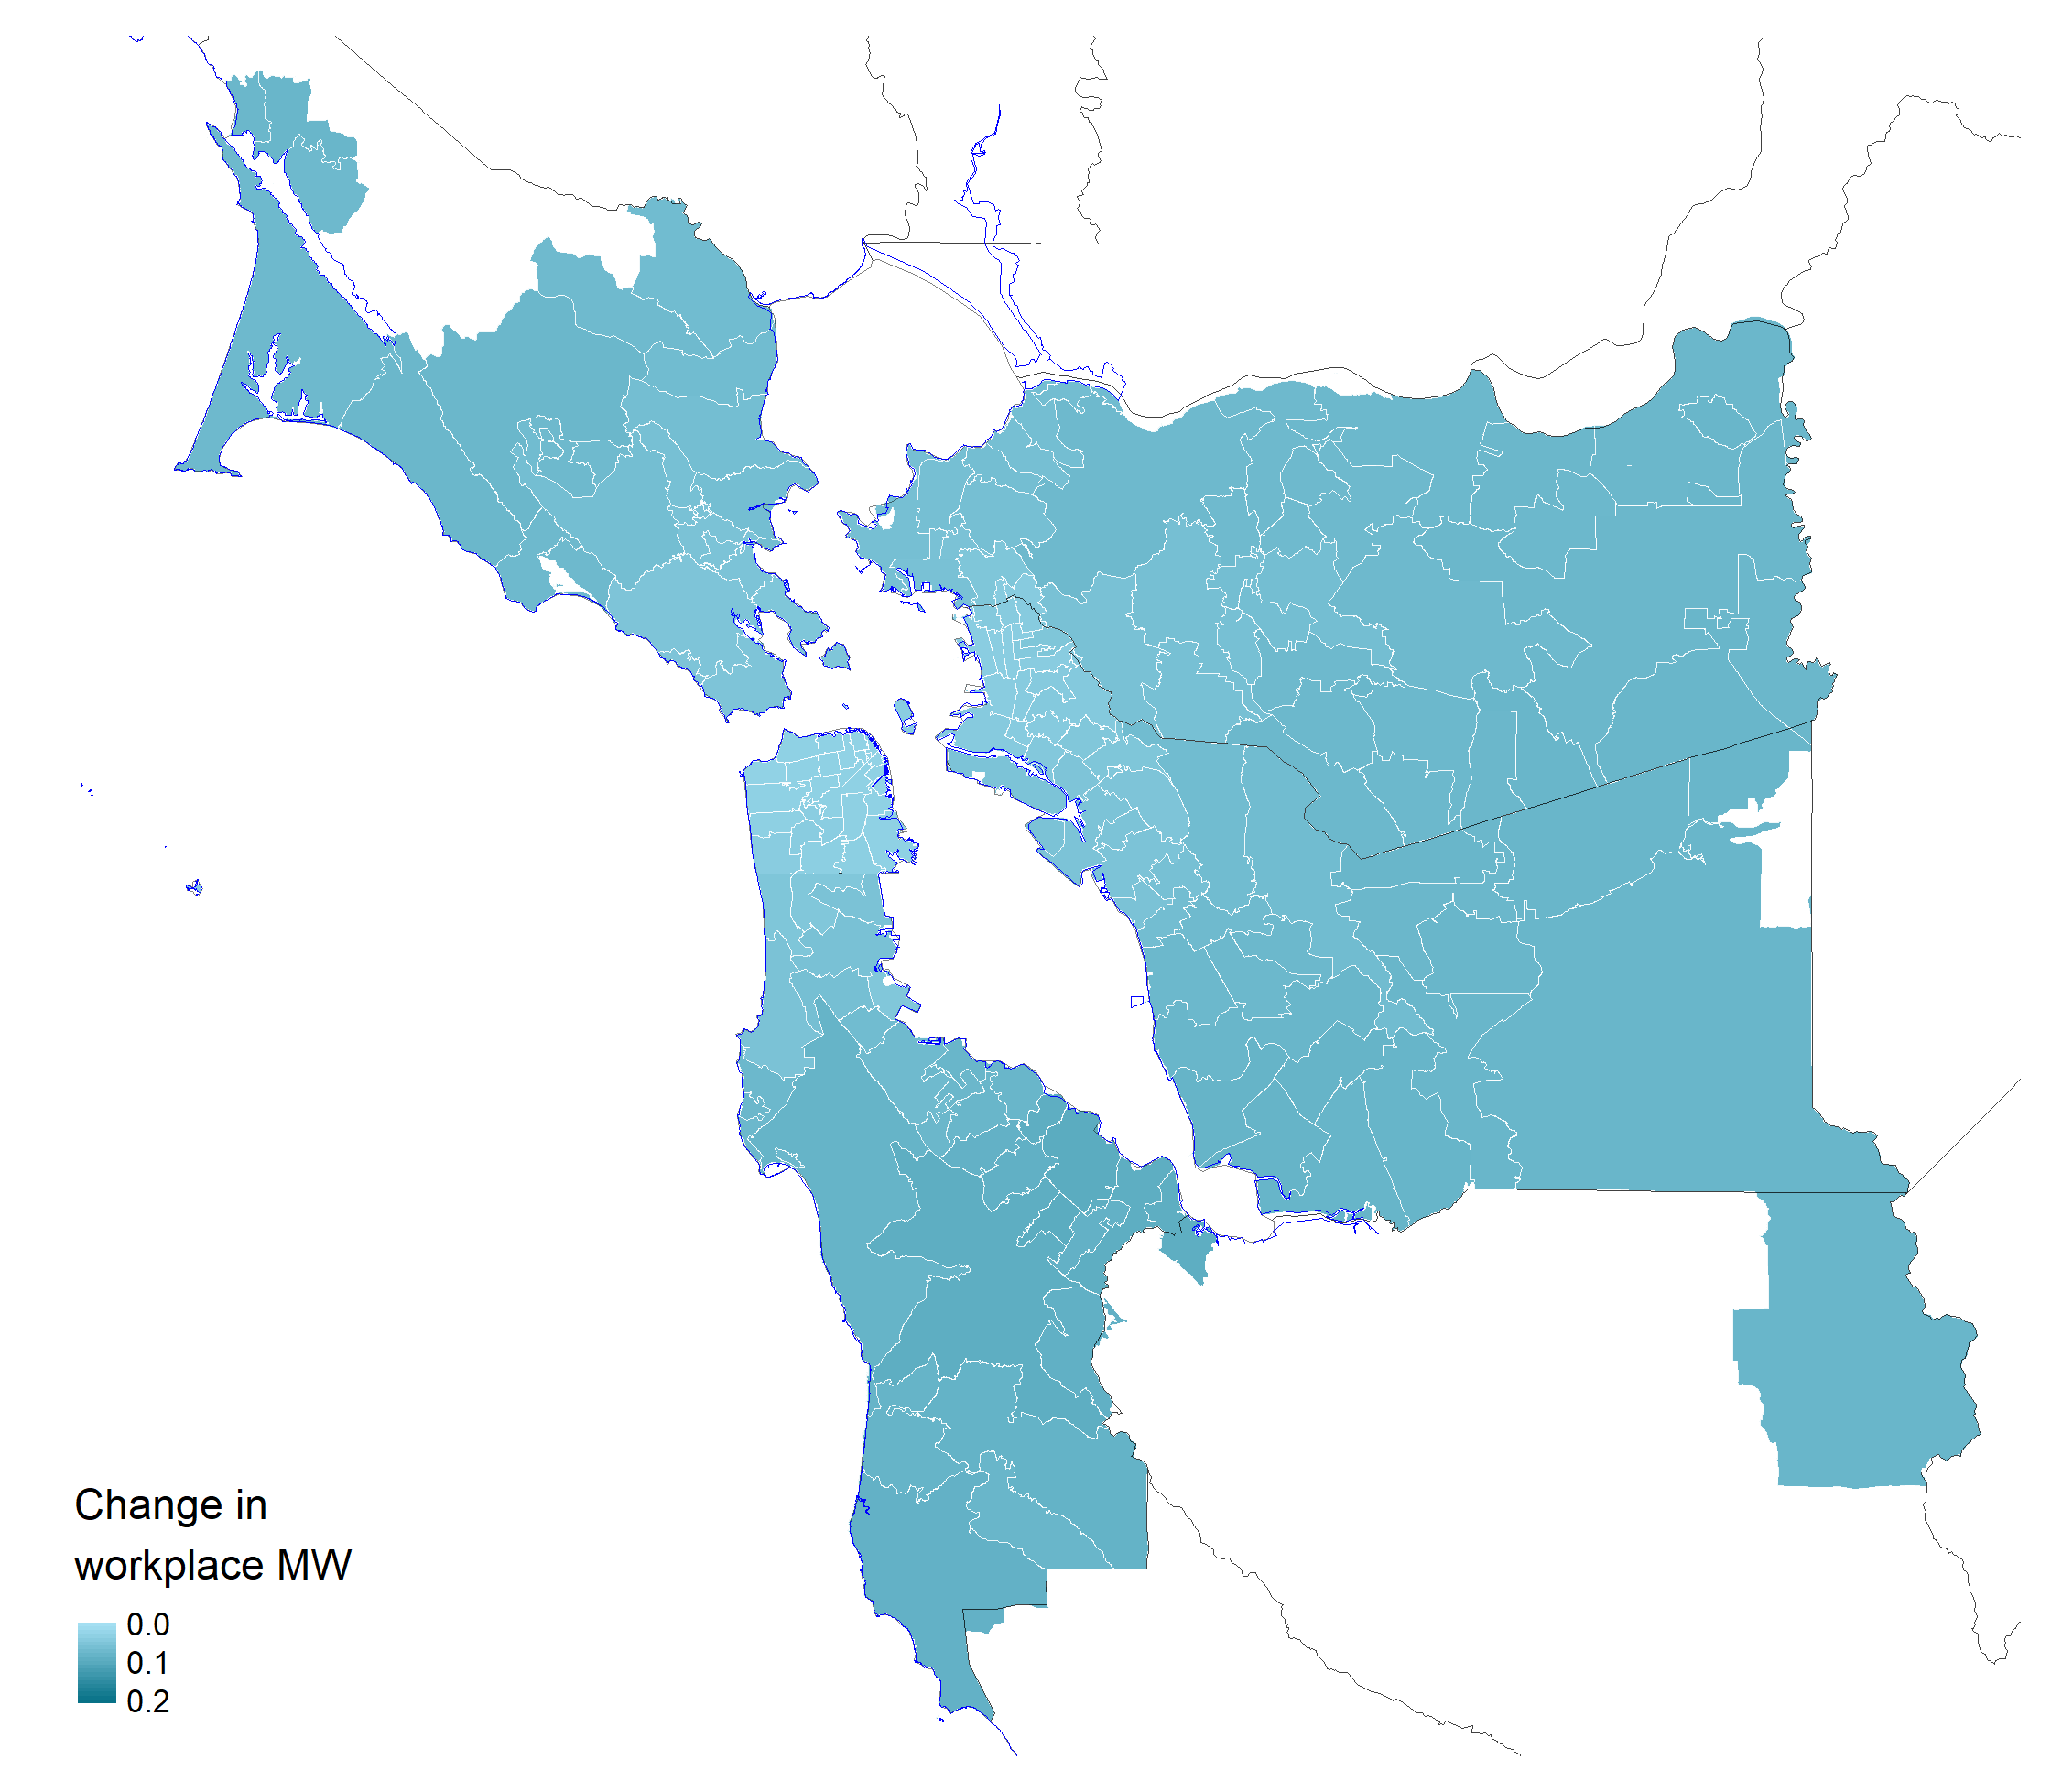
\includegraphics[scale = 0.36]{maps_events/output/bay_area2018-12_wkp_mw.png}
            \end{figure}   
        \end{column}
    \end{columns}
    \hyperlink{chi_example}{\beamerbutton{Go back}}
\end{frame}


\begin{frame}[label = san_diego_example]
\frametitle{San Diego (MW changes in January 2019)}
    \begin{columns}
        \begin{column}{0.50\textwidth}
            \vspace{-4mm}
            \begin{figure}
                \centering
                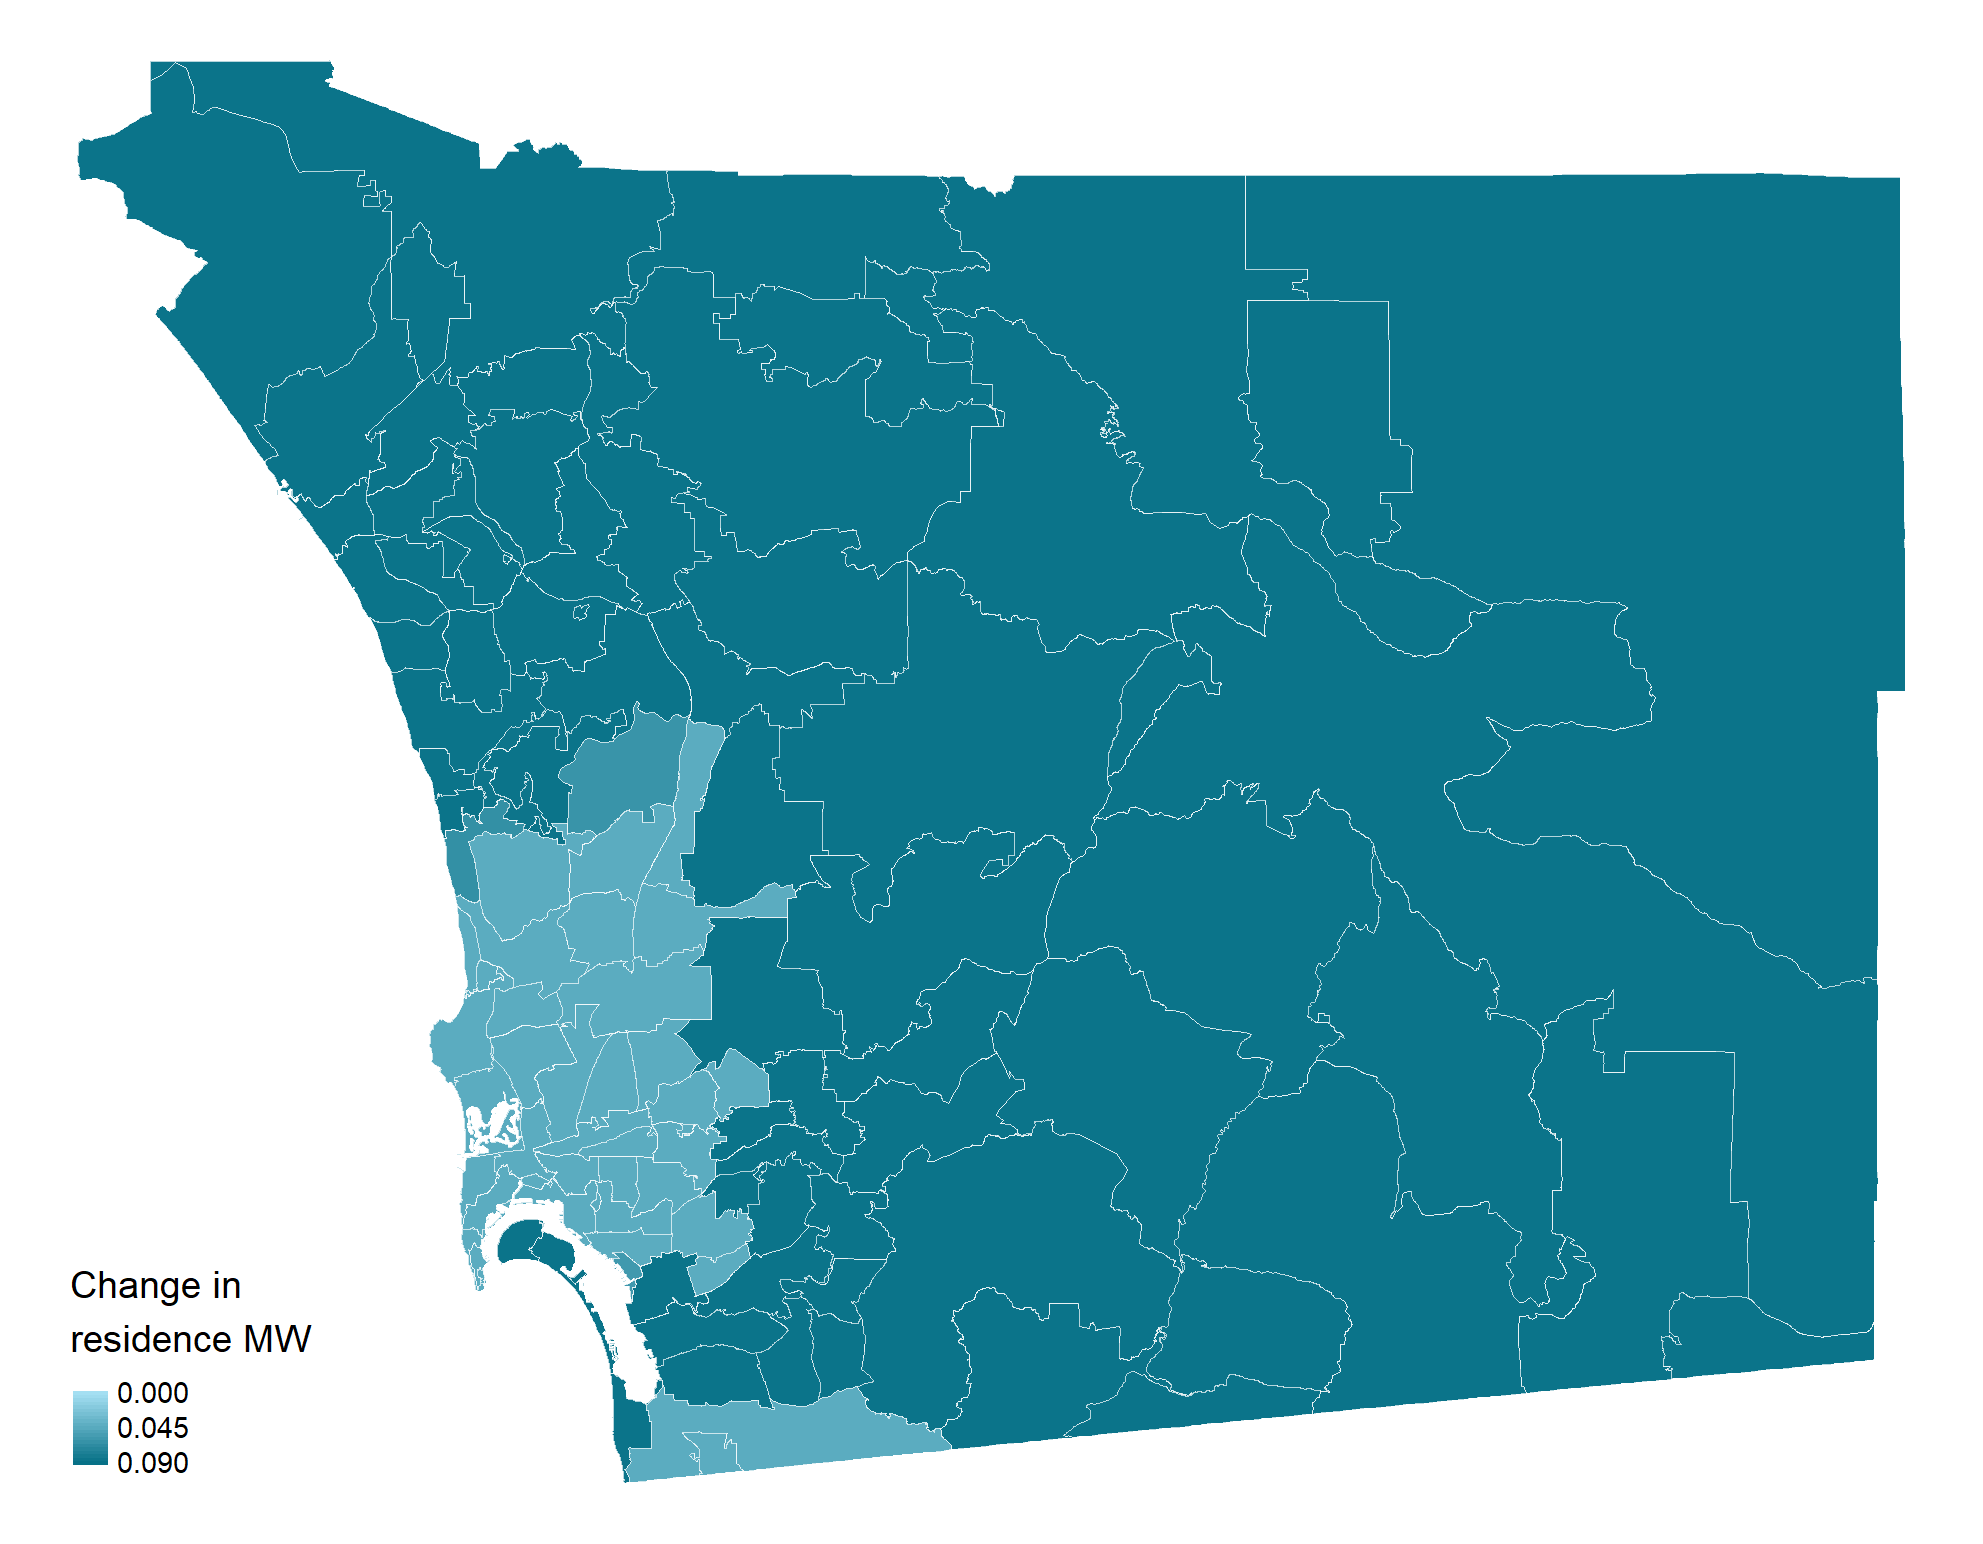
\includegraphics[scale = 0.3]{maps_events/output/san_diego_2018-12_statutory_mw.png}
            \end{figure}   
        \end{column}
        \begin{column}{0.50\textwidth}
            \vspace{-4mm}
            \begin{figure}
                \centering
                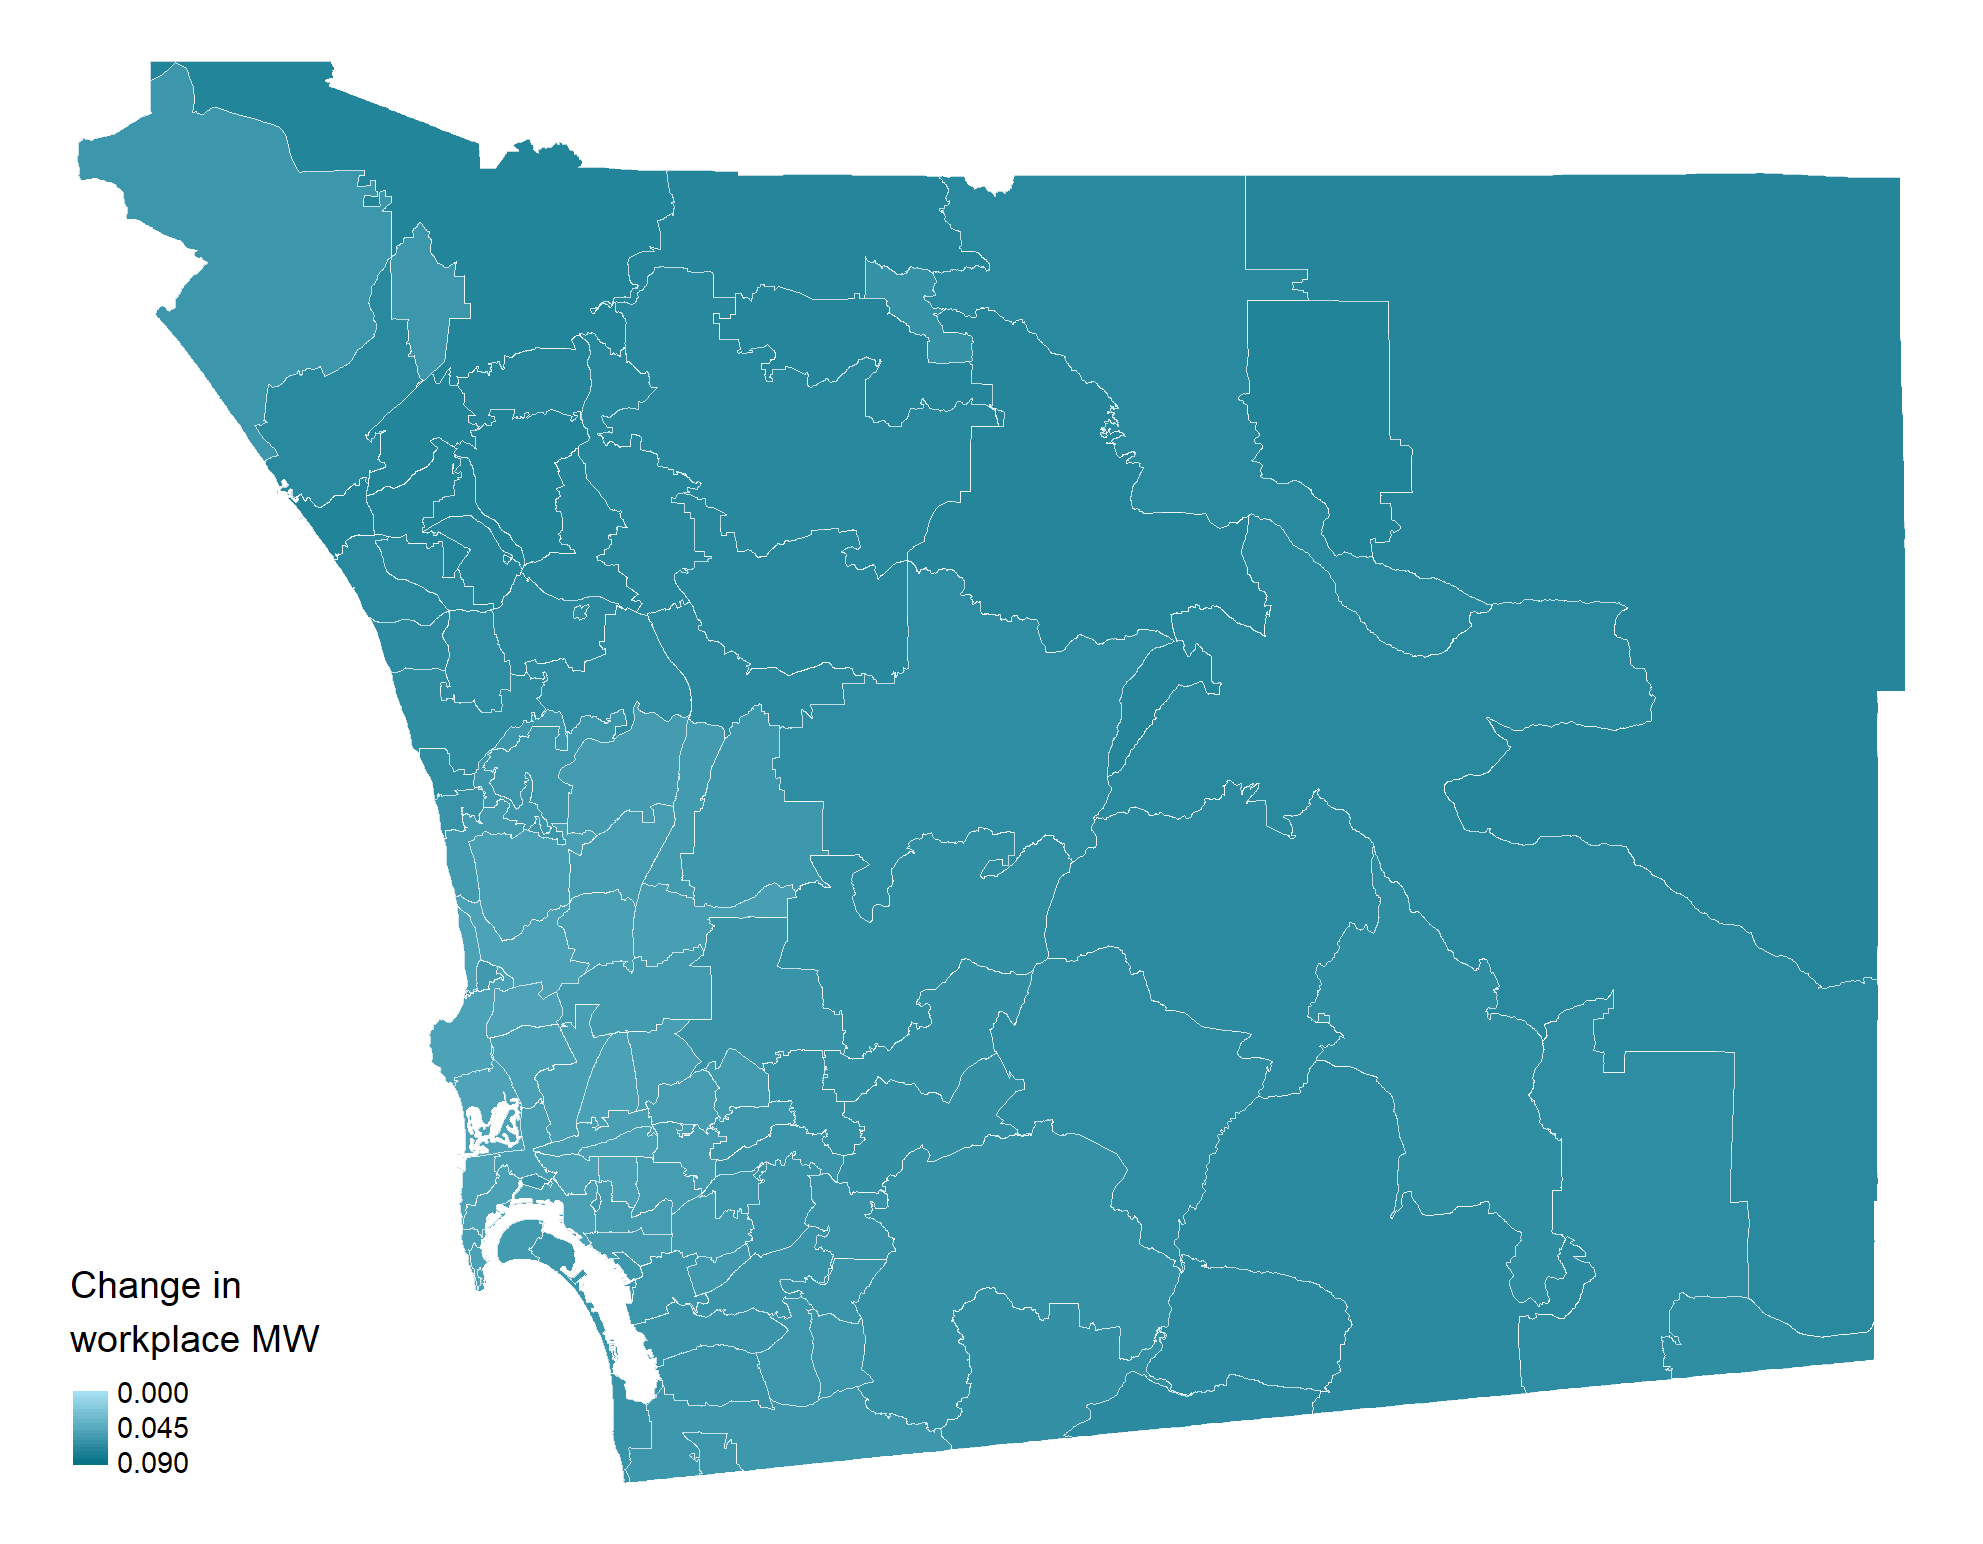
\includegraphics[scale = 0.3]{maps_events/output/san_diego2018-12_wkp_mw.png}
            \end{figure}   
        \end{column}
    \end{columns}
     \hyperlink{chi_example}{\beamerbutton{Go back}}
\end{frame}

\begin{frame}[label = kc_example]
\frametitle{Kansas City (MW changes in January 2019)}
    \begin{columns}
        \begin{column}{0.50\textwidth}
            \vspace{-4mm}
            \begin{figure}
                \centering
                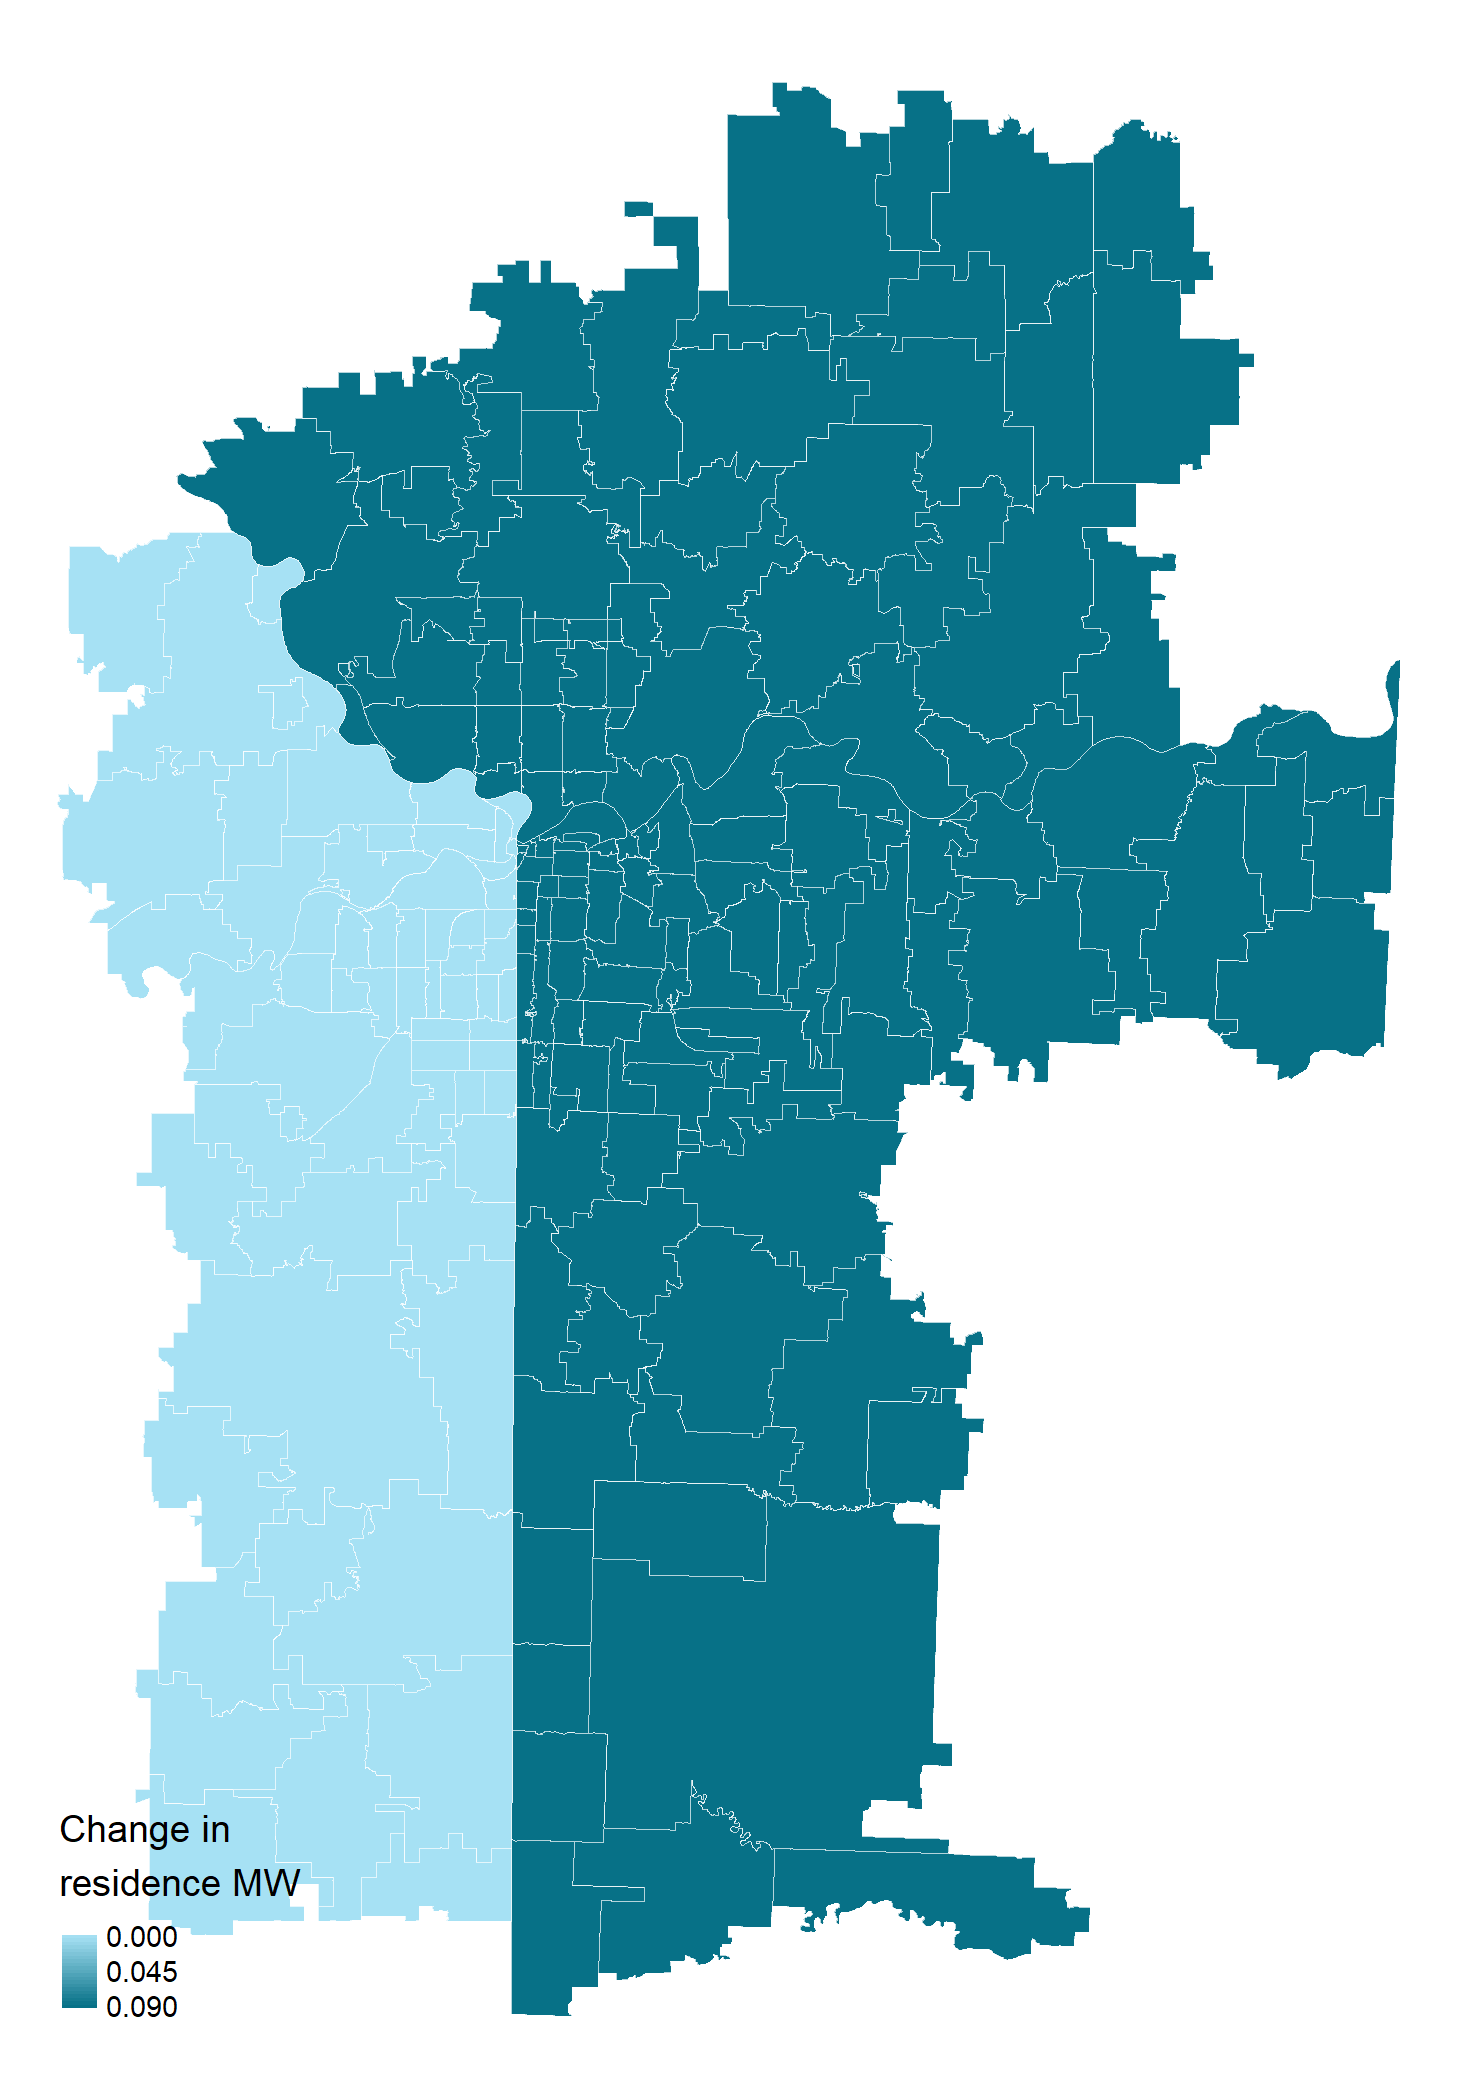
\includegraphics[scale = 0.3]{maps_events/output/kc_2018-12_statutory_mw.png}
            \end{figure}   
        \end{column}
        \begin{column}{0.50\textwidth}
            \vspace{-4mm}
            \begin{figure}
                \centering
                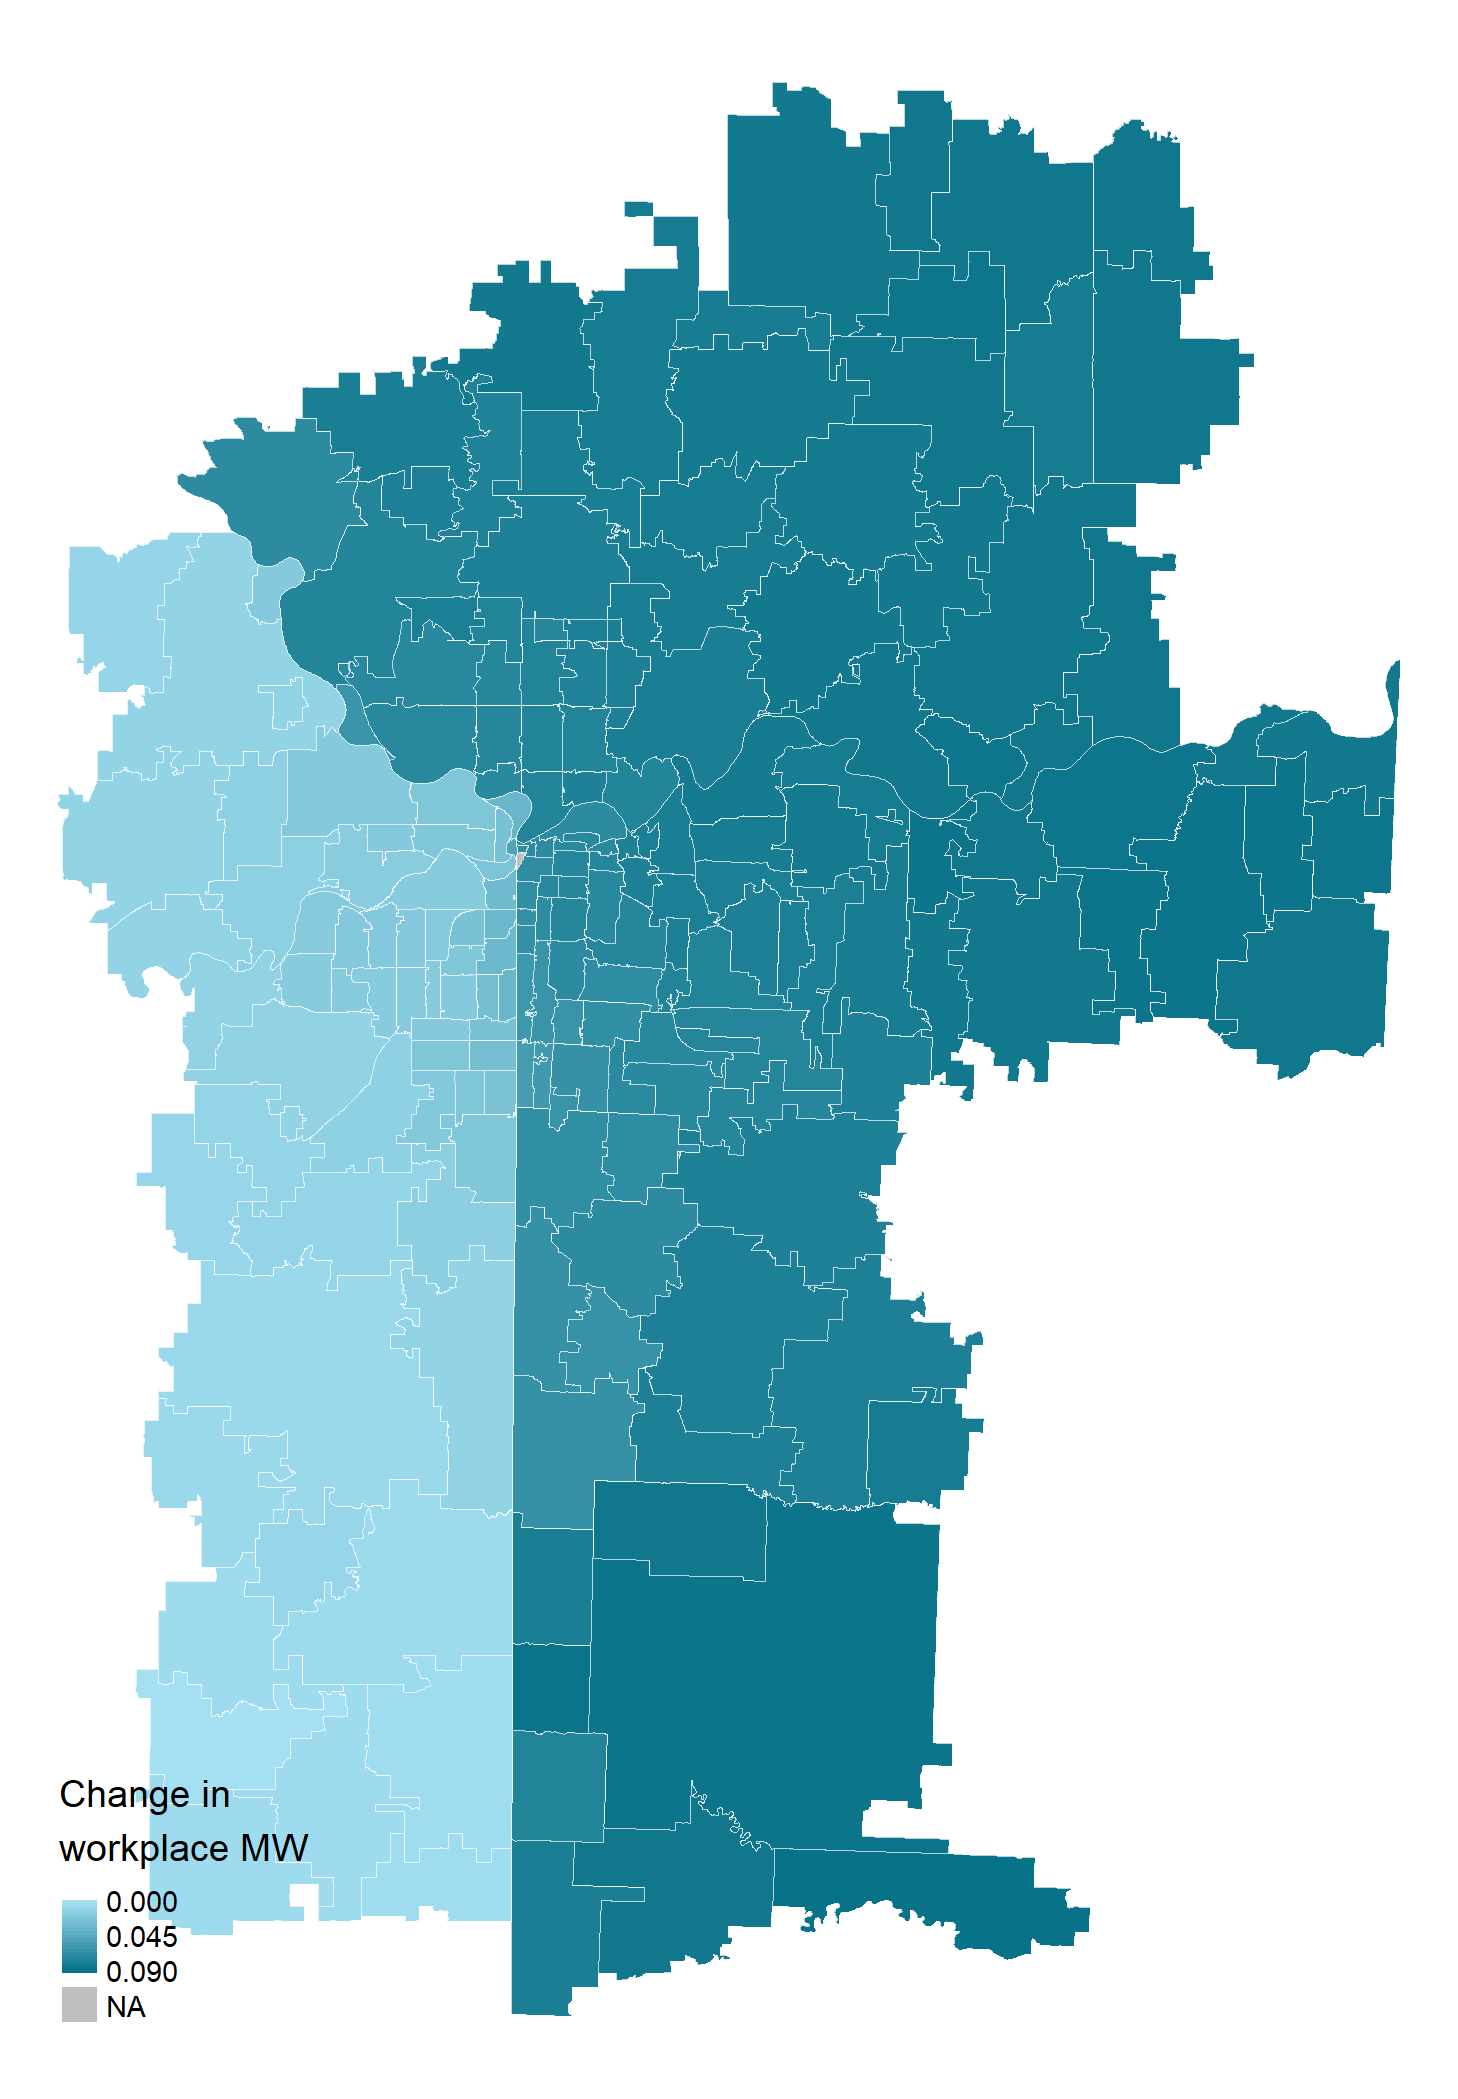
\includegraphics[scale = 0.3]{maps_events/output/kc2018-12_wkp_mw.png}
            \end{figure}   
        \end{column}
    \end{columns}
     \hyperlink{chi_example}{\beamerbutton{Go back}}
\end{frame}

\begin{frame}[label = zillow_pop_density]
    \frametitle{Comparison between Zillow Sample and Population Density}
    \begin{figure}
        \centering
    \vspace{10mm}
    \hspace{-23mm}
        \begin{subfigure}{0.41\textwidth}
            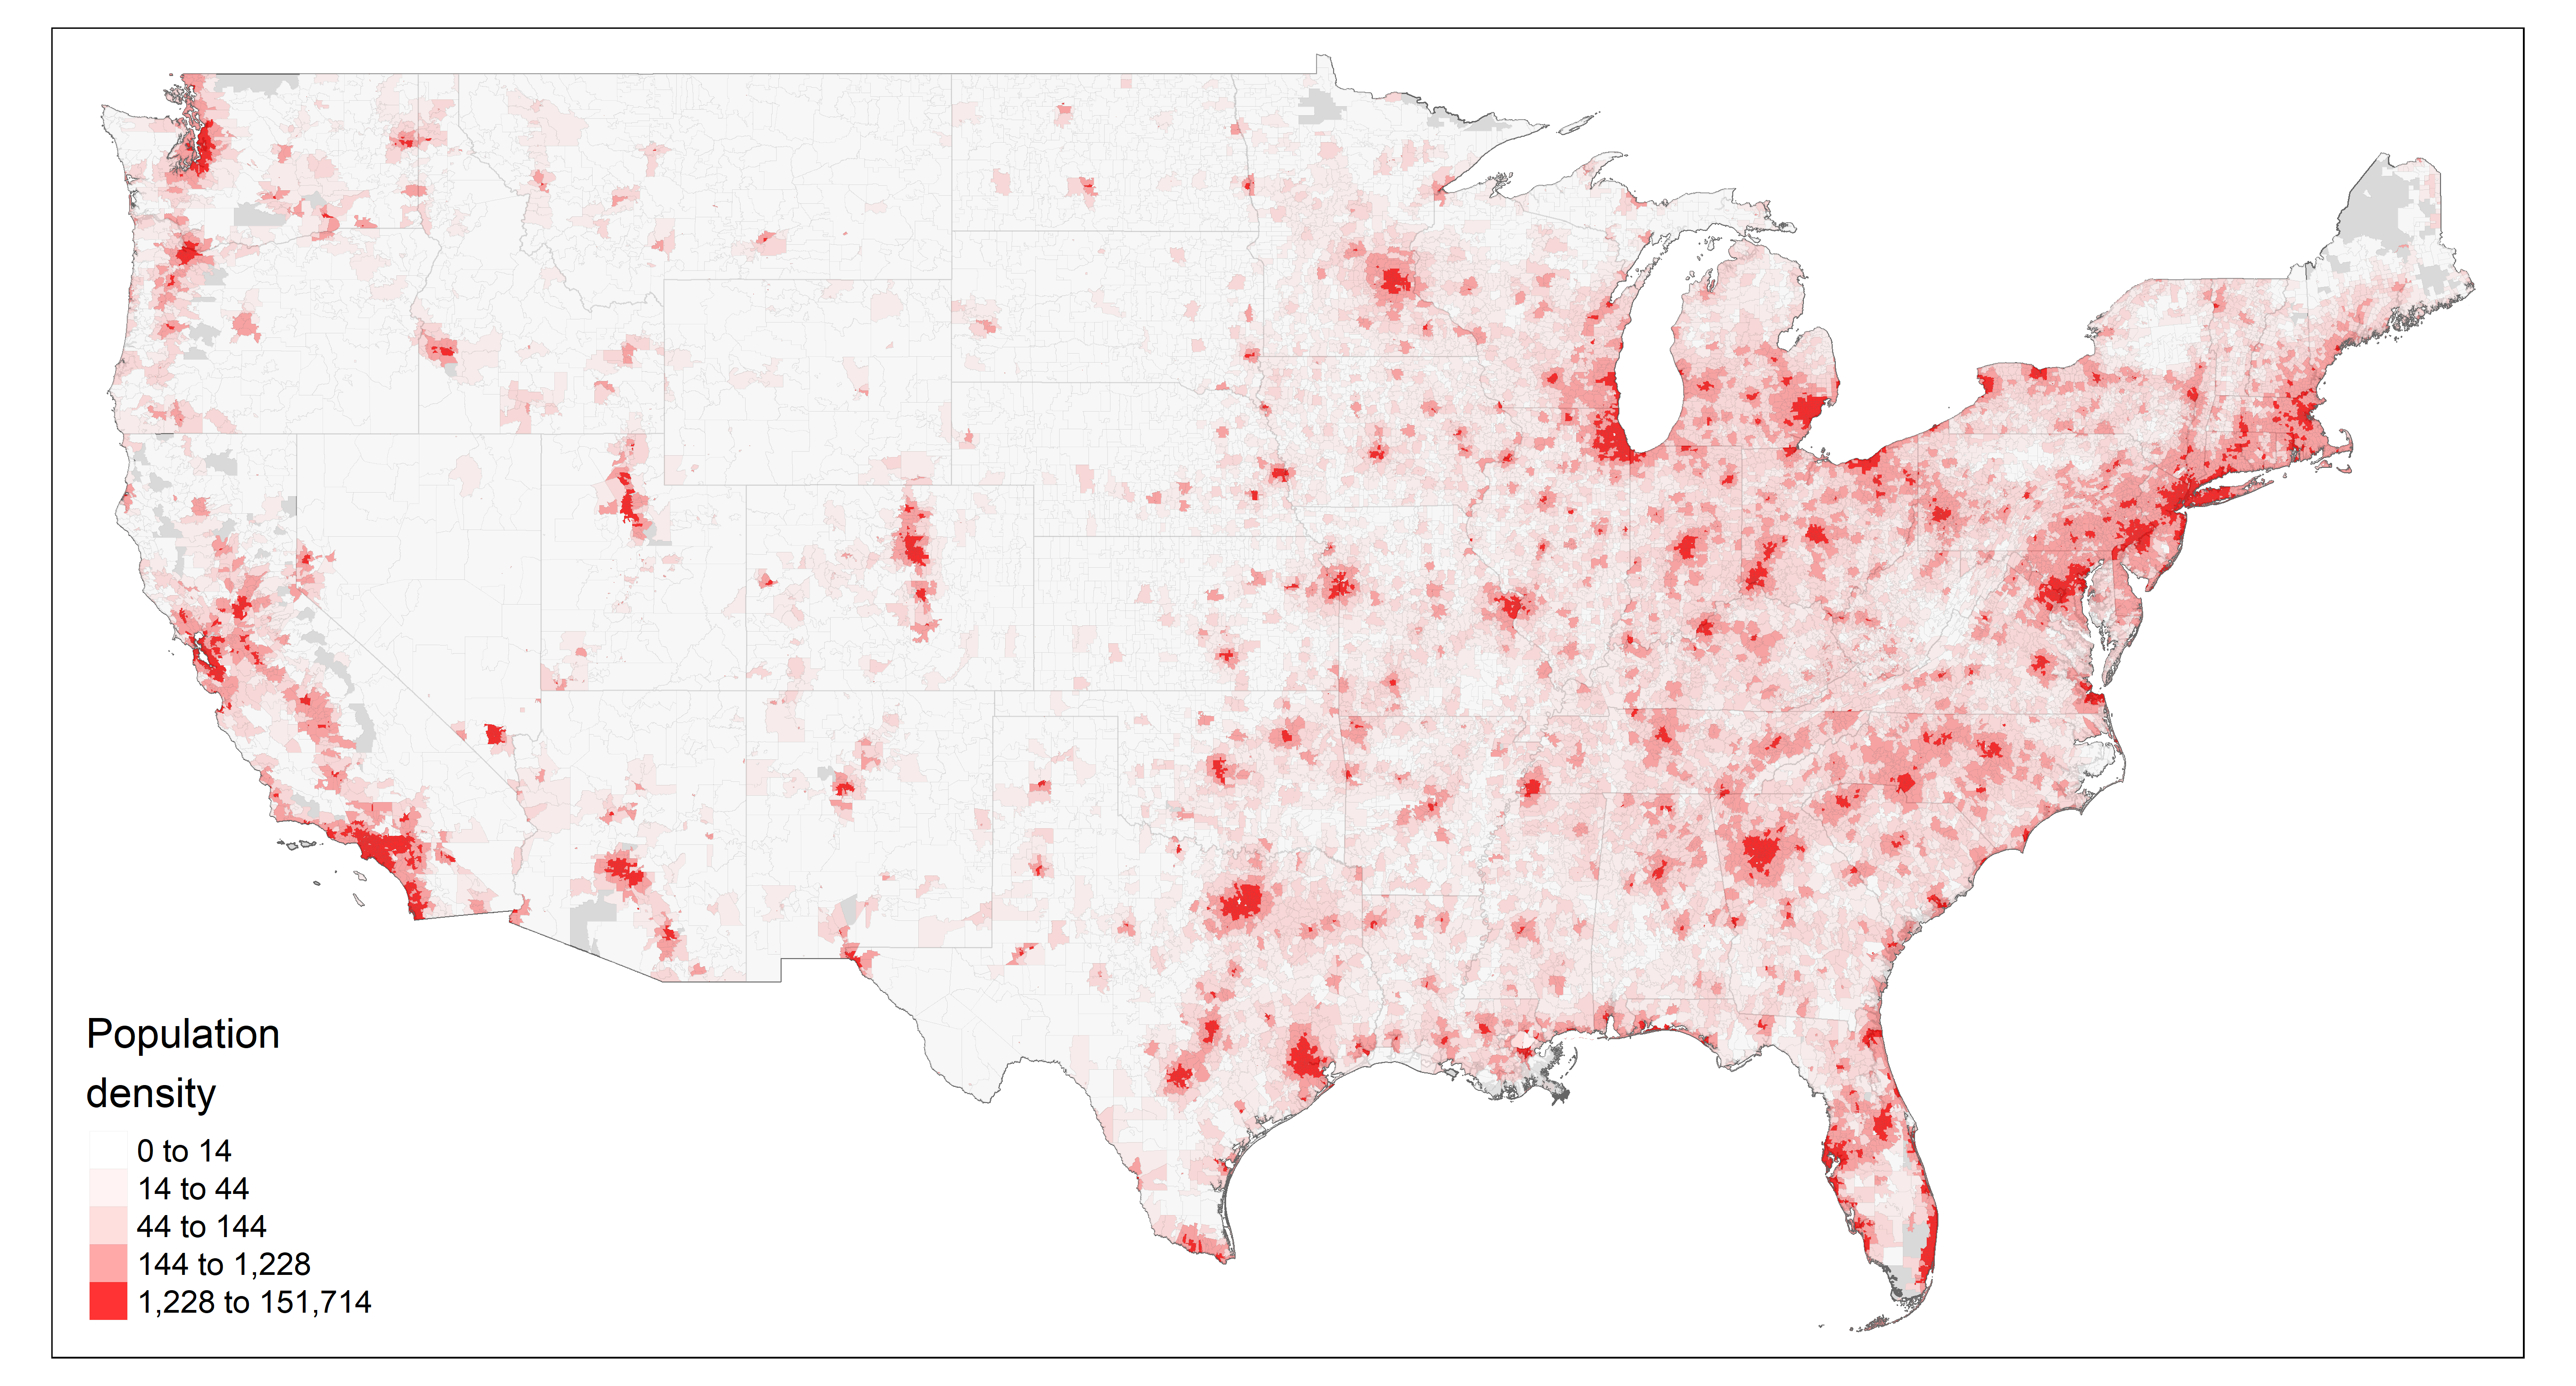
\includegraphics[scale = 0.33]{maps_US/output/USPS_zipcodes_pop_density.png}
        \end{subfigure}%
    \quad\quad\quad\quad\quad\quad
        \begin{subfigure}{0.41\textwidth}
            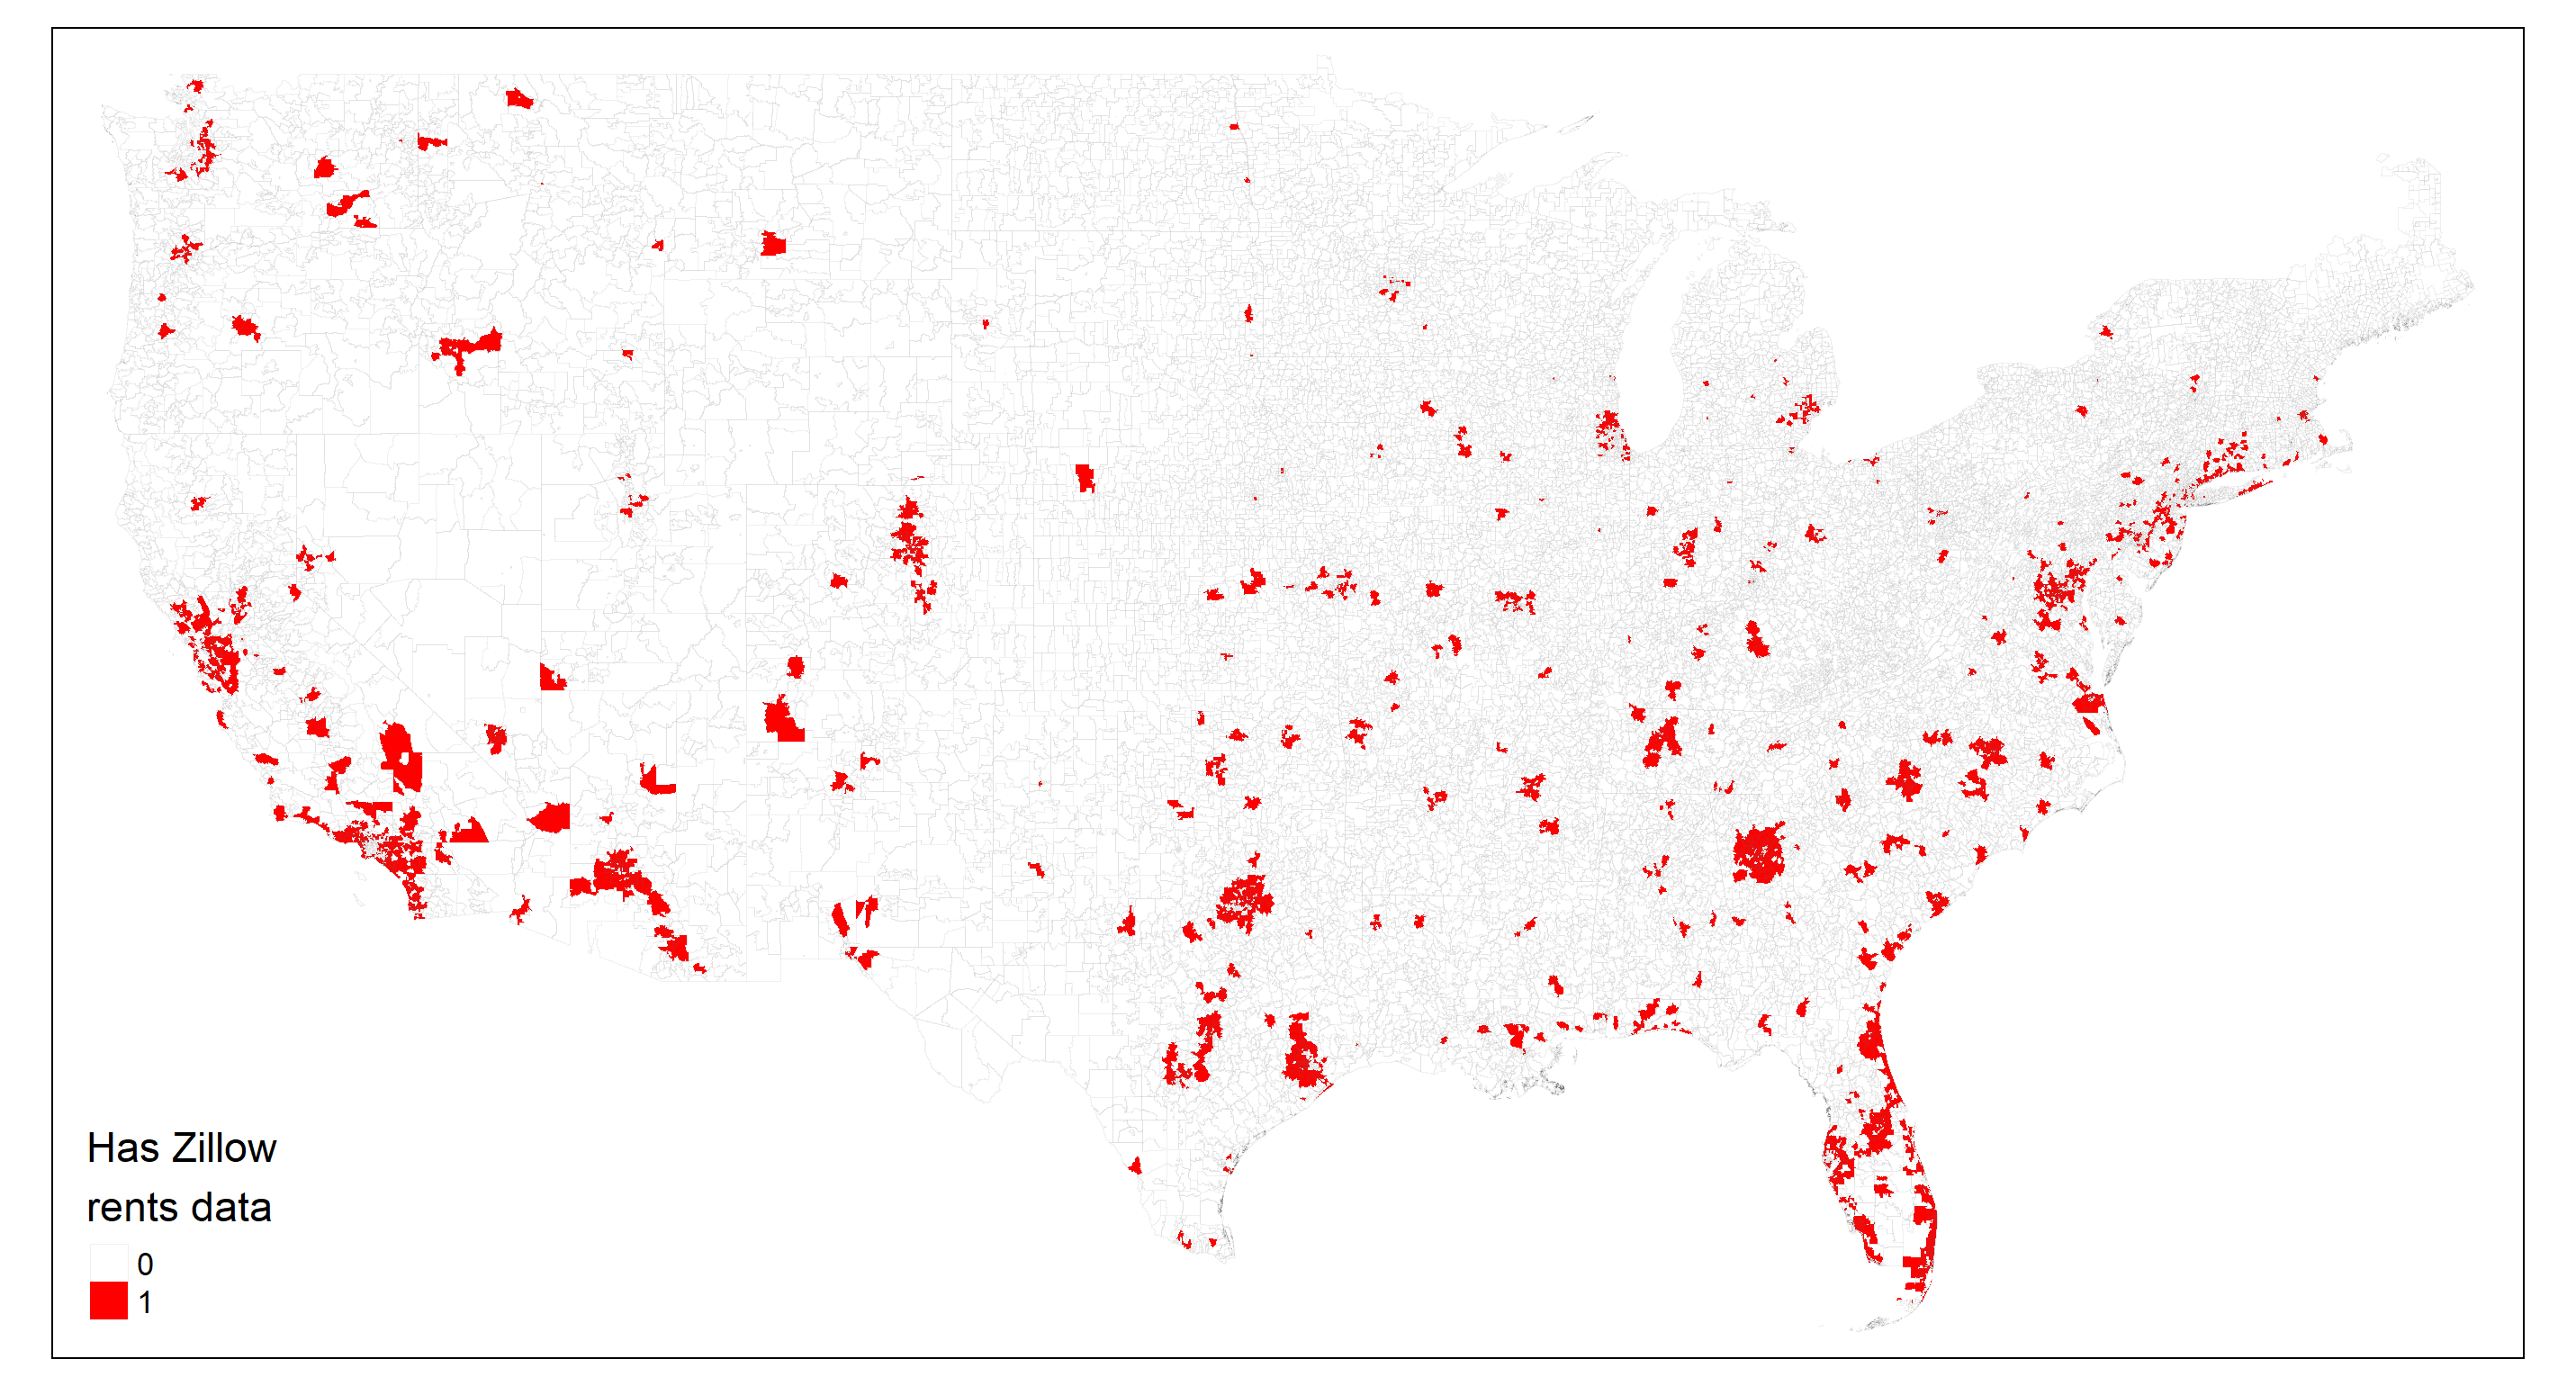
\includegraphics[scale = 0.33]{maps_US/output/USPS_zipcodes_zillow_data.png}
        \end{subfigure}
    \end{figure}
    \hyperlink{zillow_data}{\beamerbutton{Go Back}}
\end{frame}

\begin{frame}[label=dist_mw_changes]
    \frametitle{Distribution of (positive) MW changes}

    \vspace{-4mm}
    \begin{figure}
        \begin{subfigure}{0.51\textwidth}
            \vspace{6mm}
            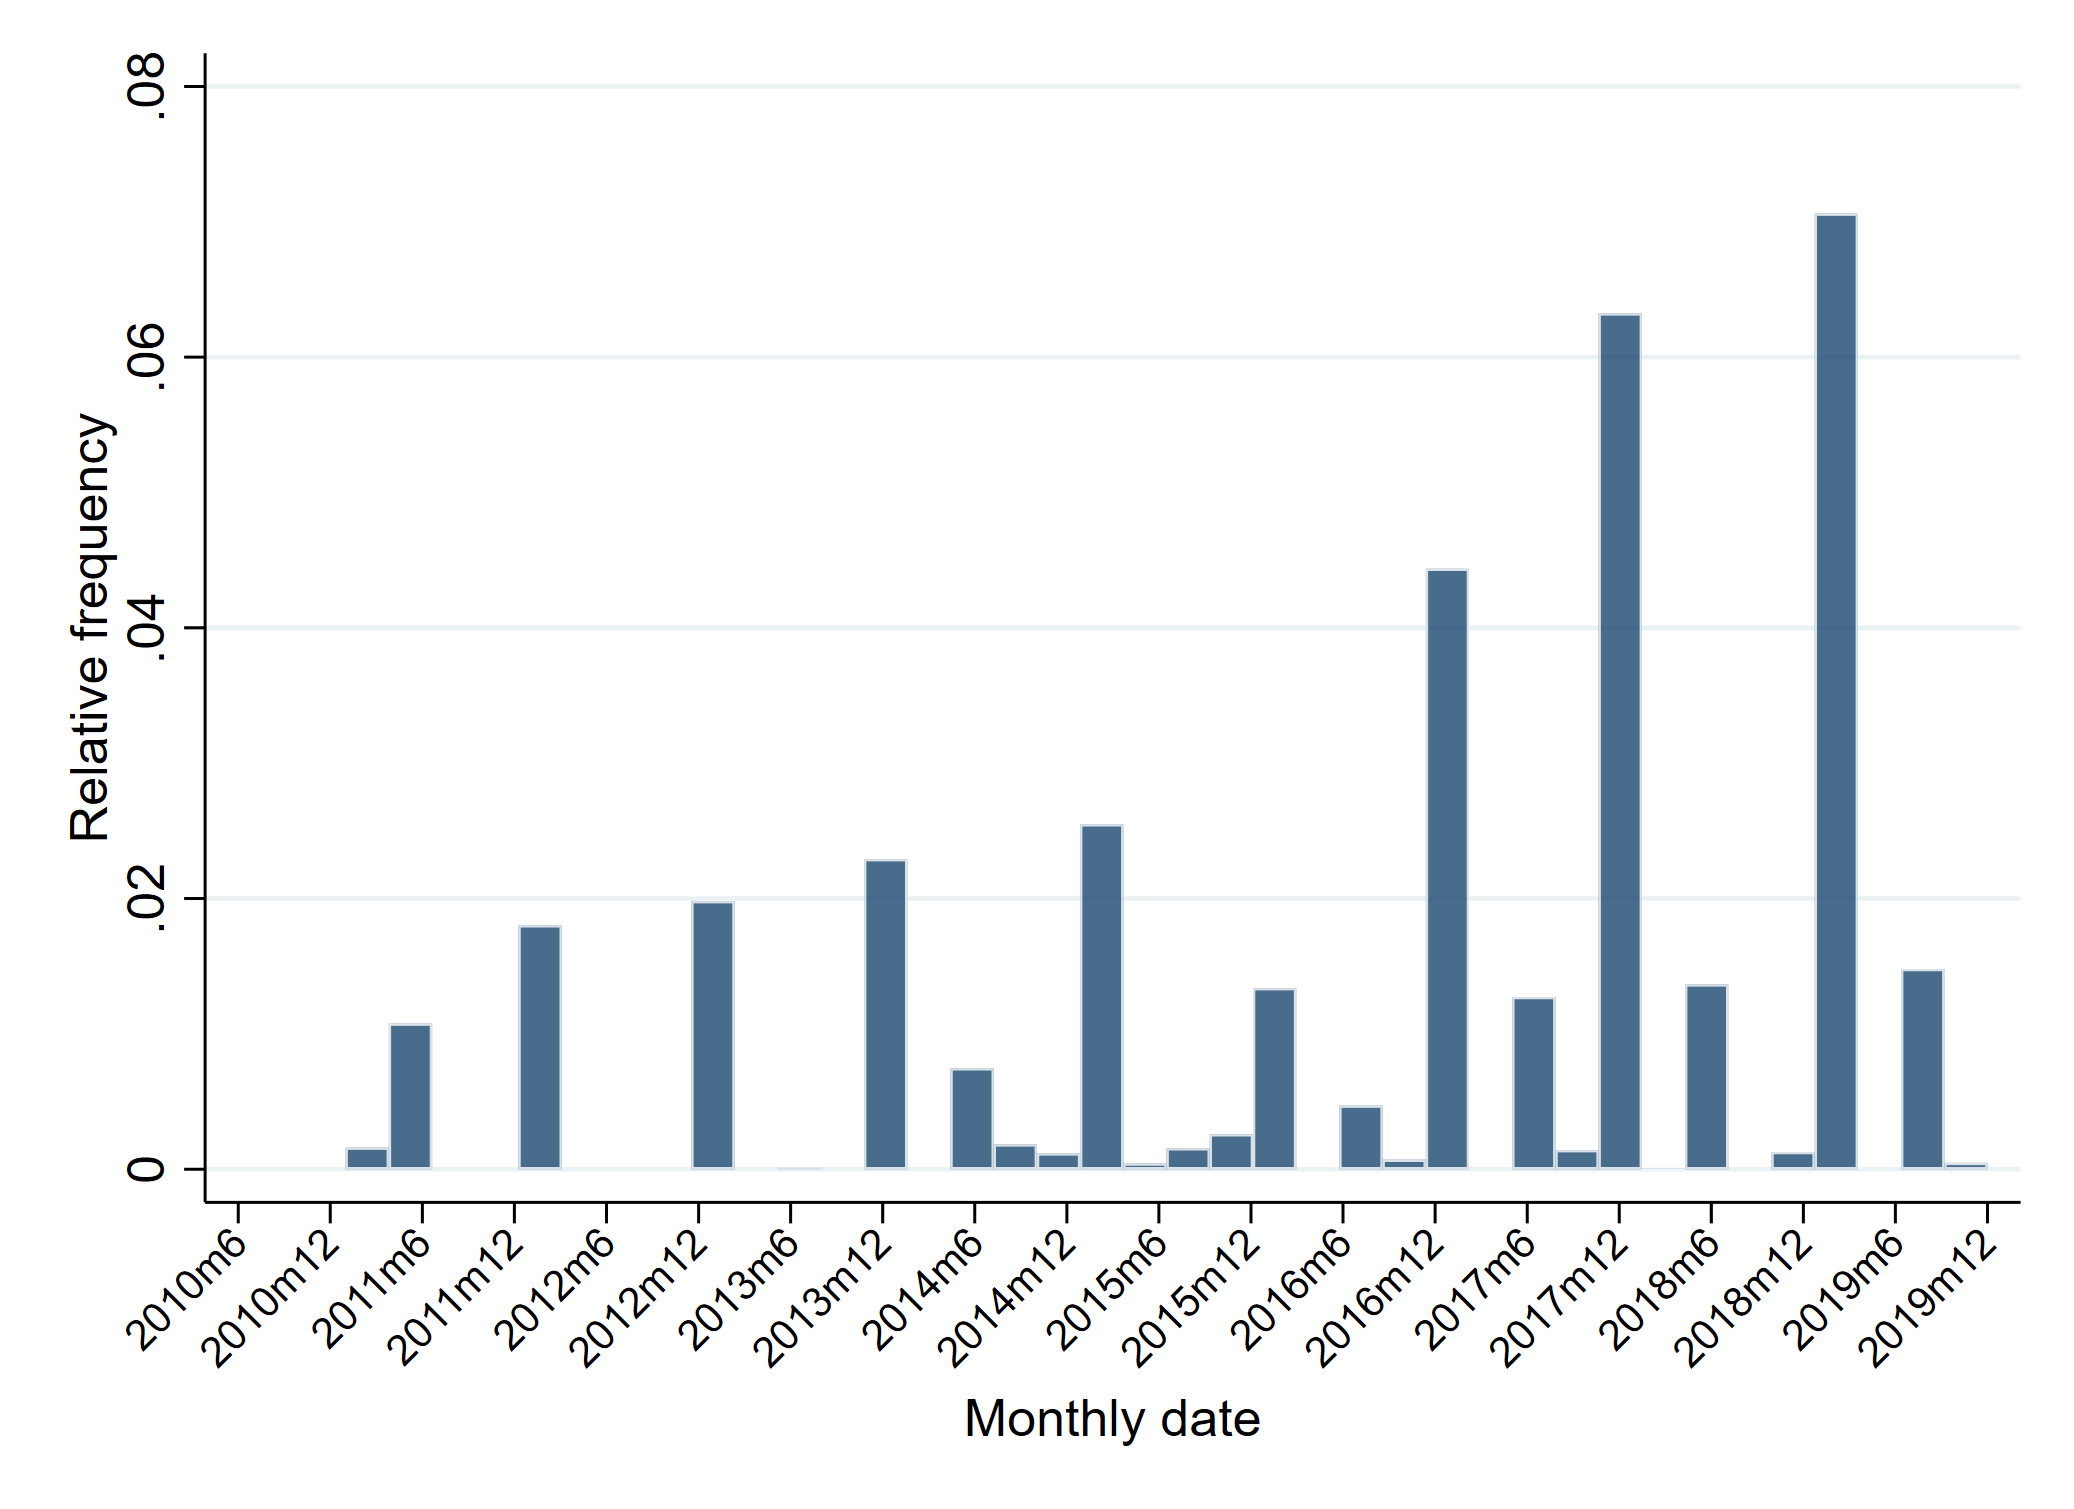
\includegraphics[width = 1.02\textwidth]{estimation_samples/output/pct_ch_mw_date_dist.png}
        \end{subfigure}%
        \begin{subfigure}{0.51\textwidth}
            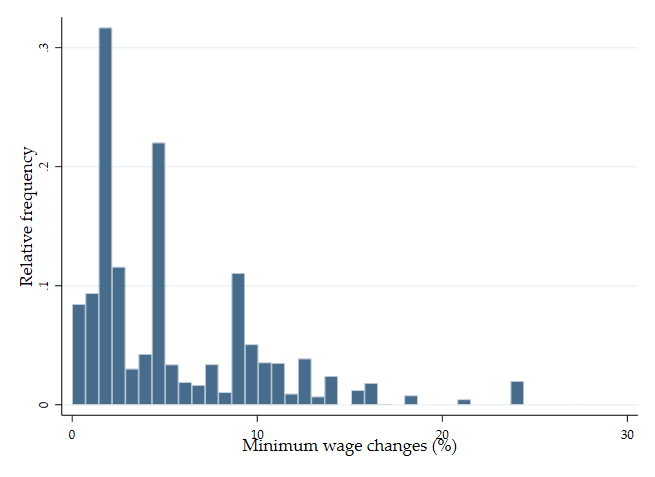
\includegraphics[width = 1.02\textwidth]{estimation_samples/output/pct_ch_mw_dist.png}
        \end{subfigure}
    \end{figure}
    
    \hyperlink{dist_mw_changes}{\beamerbutton{Go Back}}
\end{frame}

\begin{frame}[label=mw_changes_map]
    \frametitle{MW changes between Jan 2010 and Dec 2019, mainland US}

    \vspace{2mm}
    \begin{figure}        
        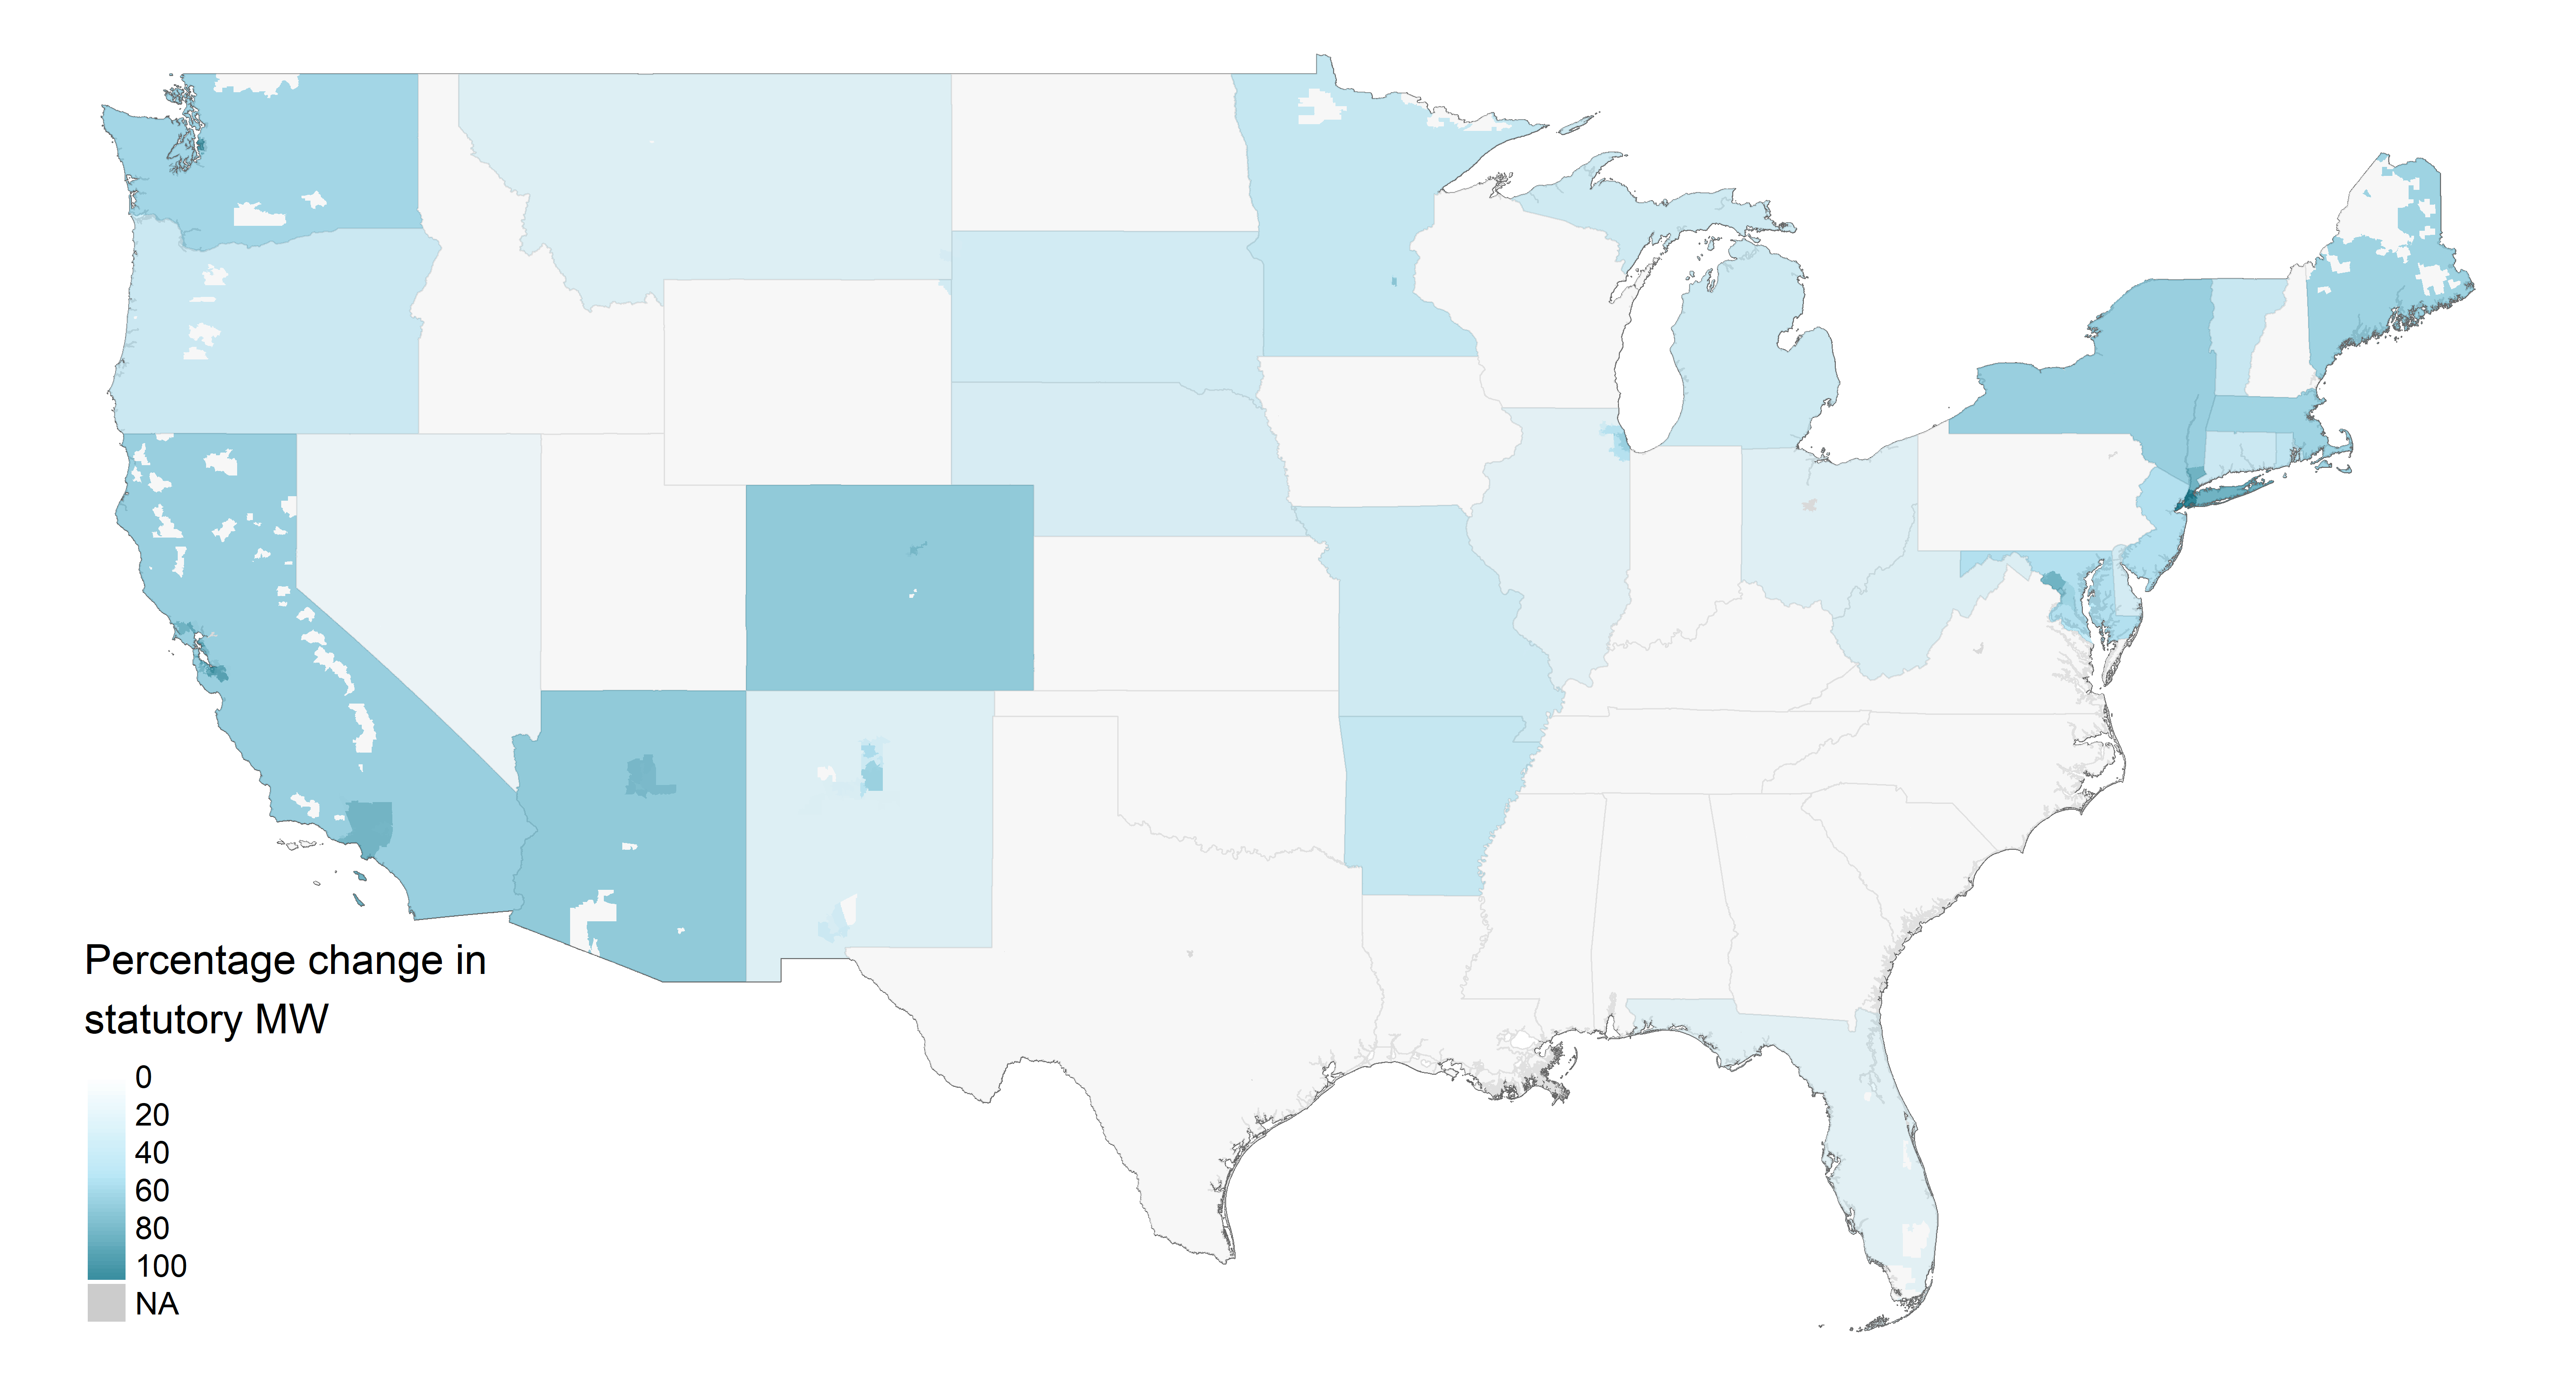
\includegraphics[width = 0.84\textwidth]{maps_mw_long_run/output/USchange_perc_statutory_mw.png}
    \end{figure}
    
    \hyperlink{dist_mw_changes}{\beamerbutton{Go Back}}
\end{frame}

\begin{frame}[label = exclude_res]
    \frametitle{Excluding residence MW}

    \begin{figure}
        \centering
        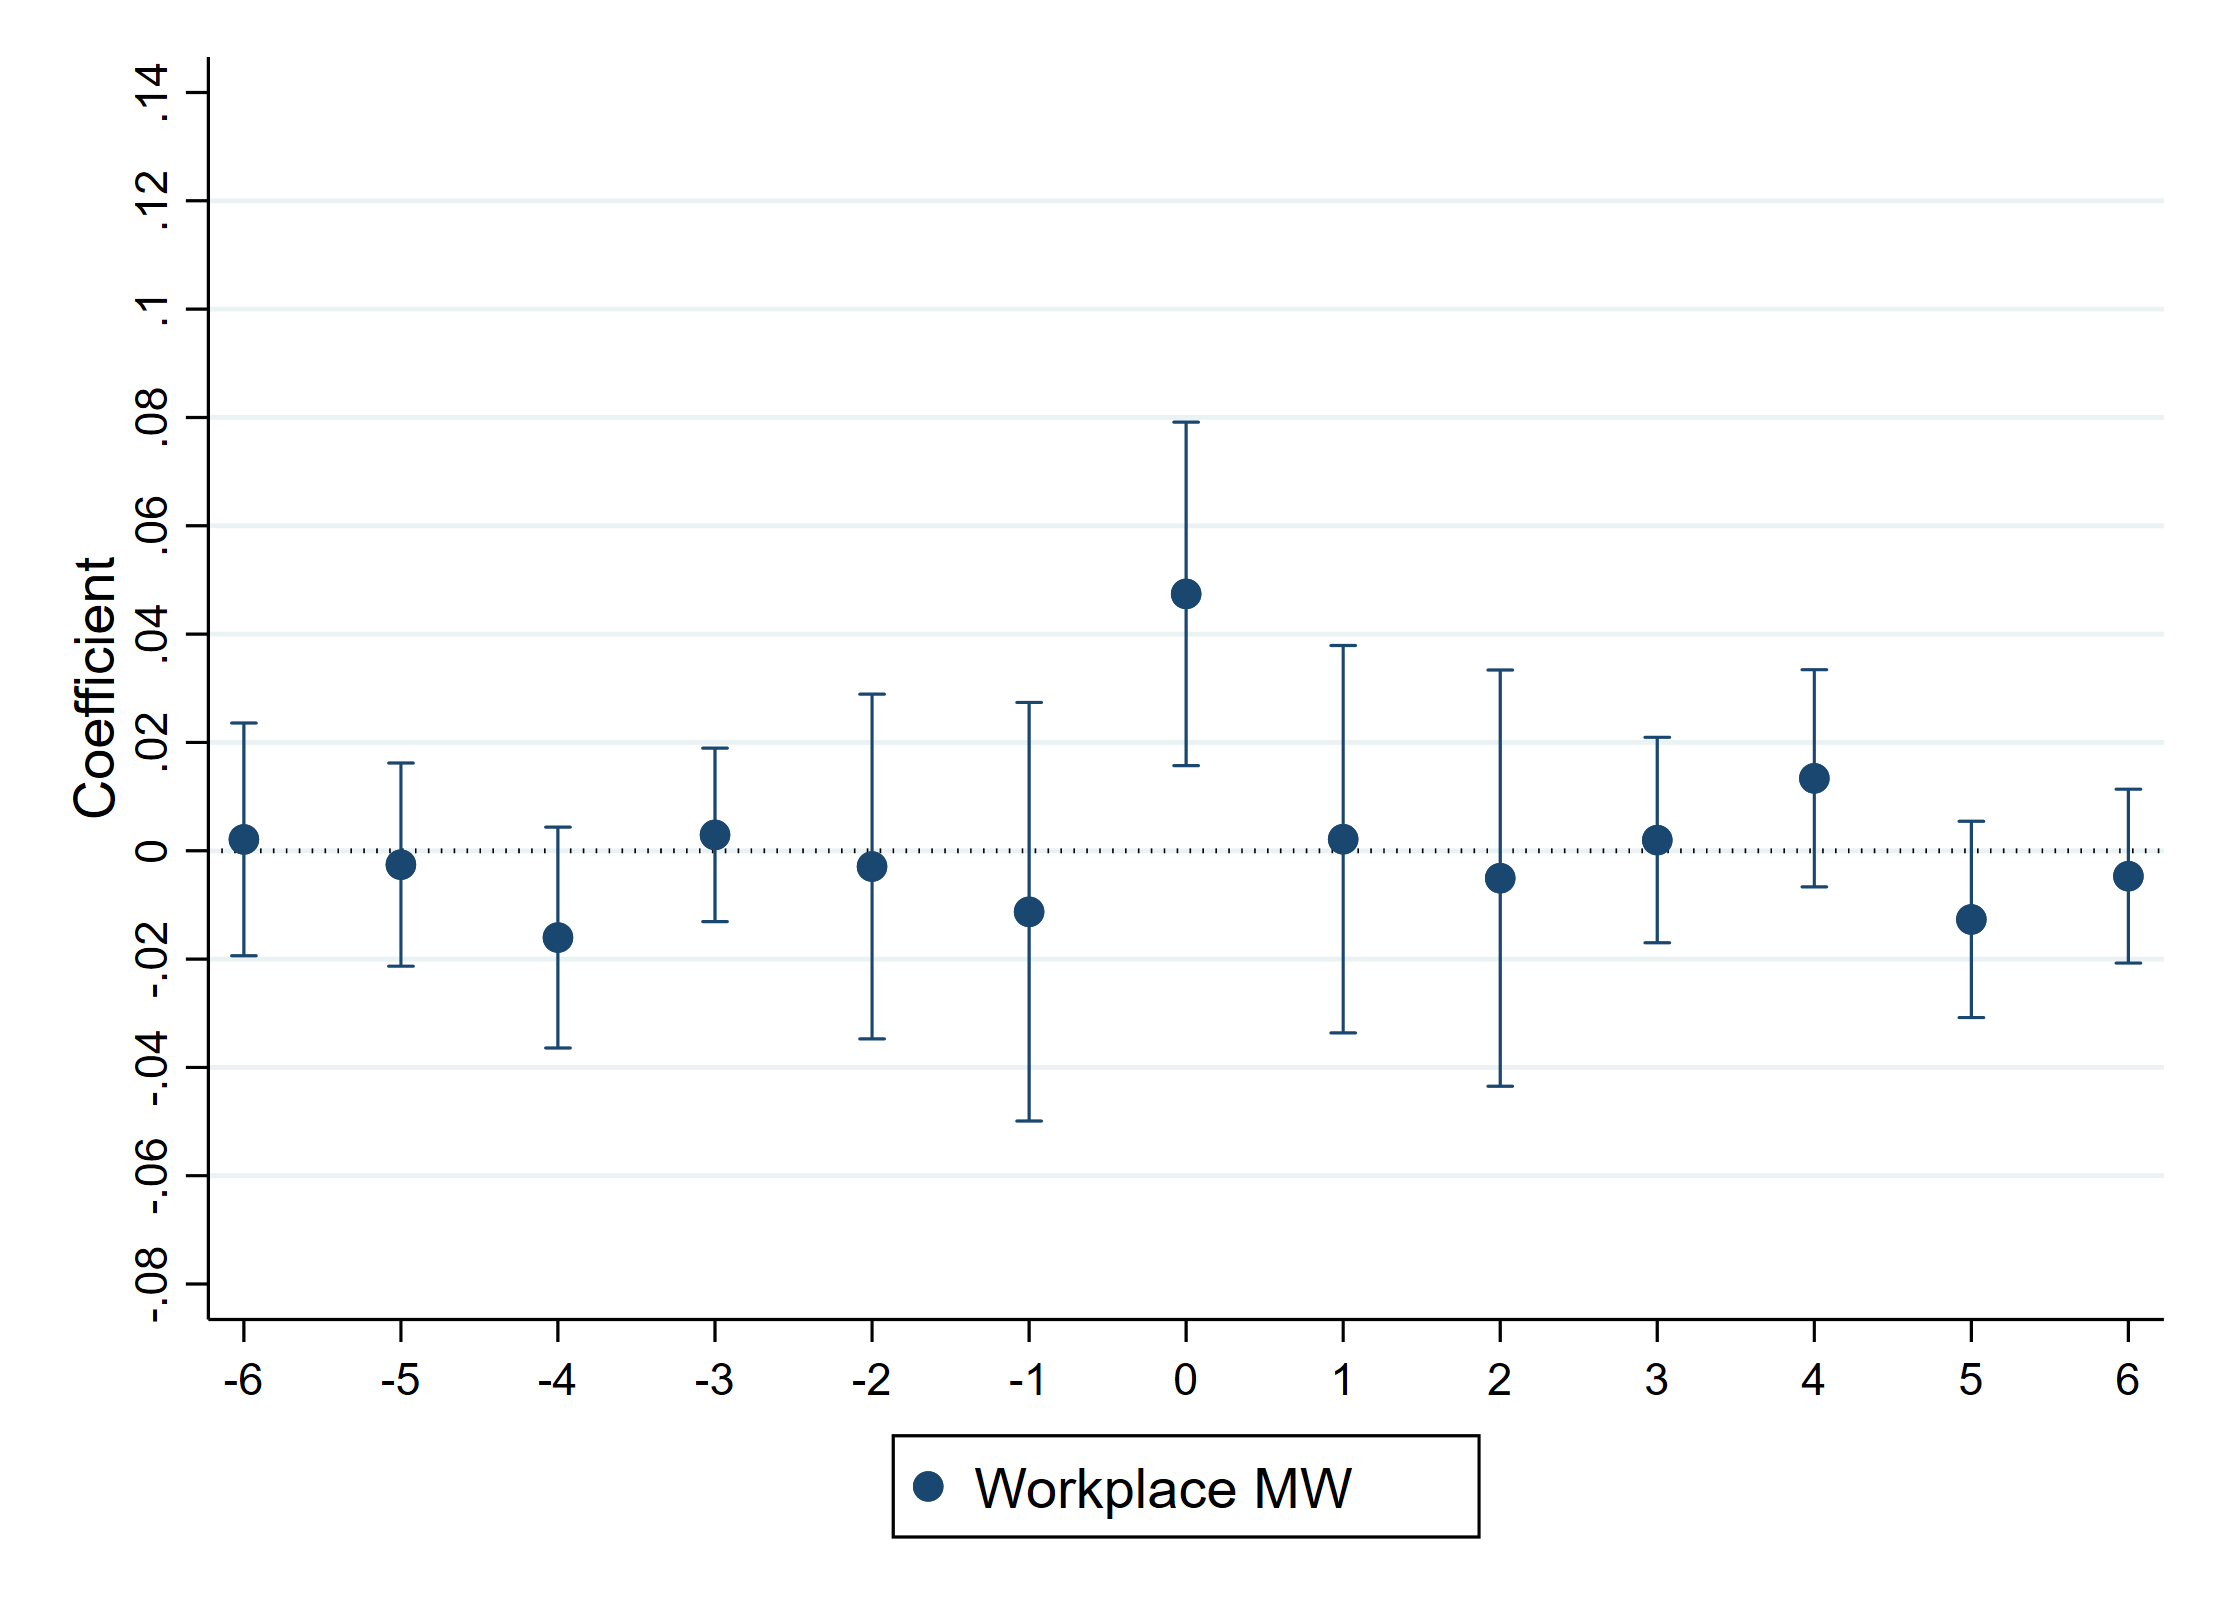
\includegraphics[width=0.68\textwidth]{fd_baseline/output/fd_mw_wkp_only_dynamic.png}
    \end{figure}
    
    \hyperlink{dyn_baseline_plot}{\beamerbutton{Go Back}}
\end{frame}

\begin{frame}[label = res_only_dyn]
    \frametitle{Including leads and lags of residence MW}

    \begin{figure}
        \centering
        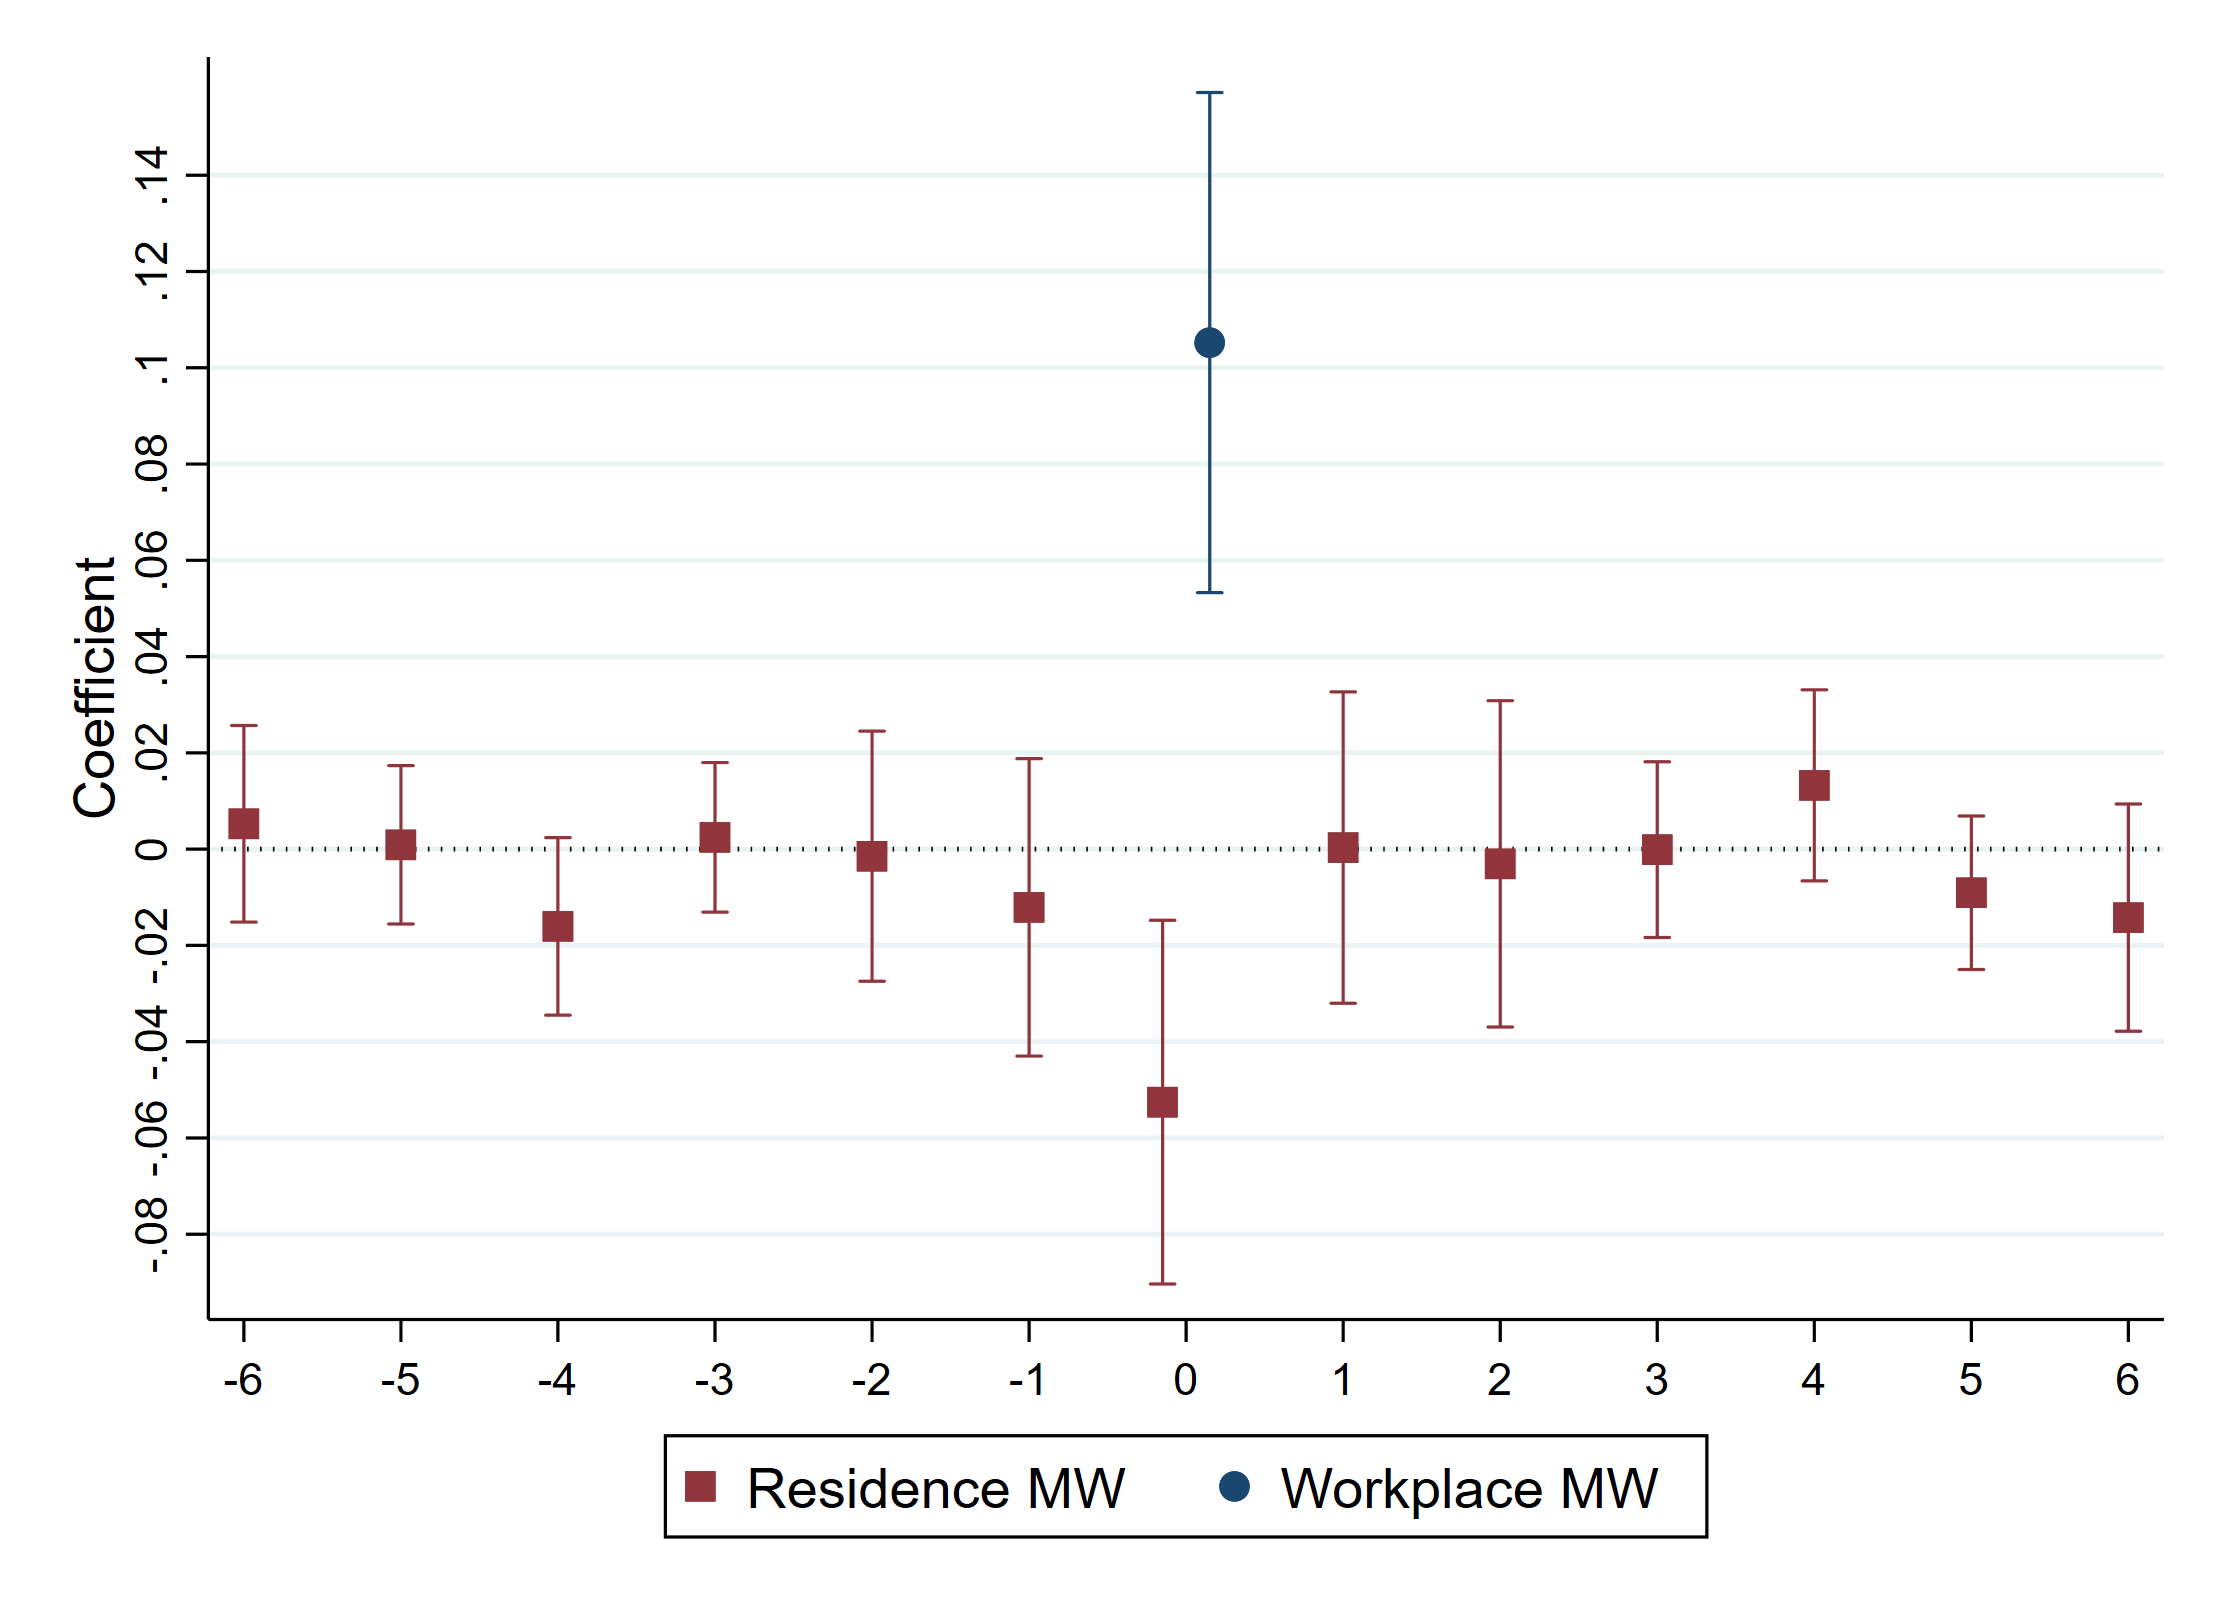
\includegraphics[width=0.68\textwidth]{fd_baseline/output/fd_both_mw_res_only_dynamic.png}
    \end{figure}
    
    \hyperlink{dyn_baseline_plot}{\beamerbutton{Go Back}}
\end{frame}

\begin{frame}[label = both_dyn]
    \frametitle{Including leads and lags of both MW measures}

    \begin{figure}
        \centering
        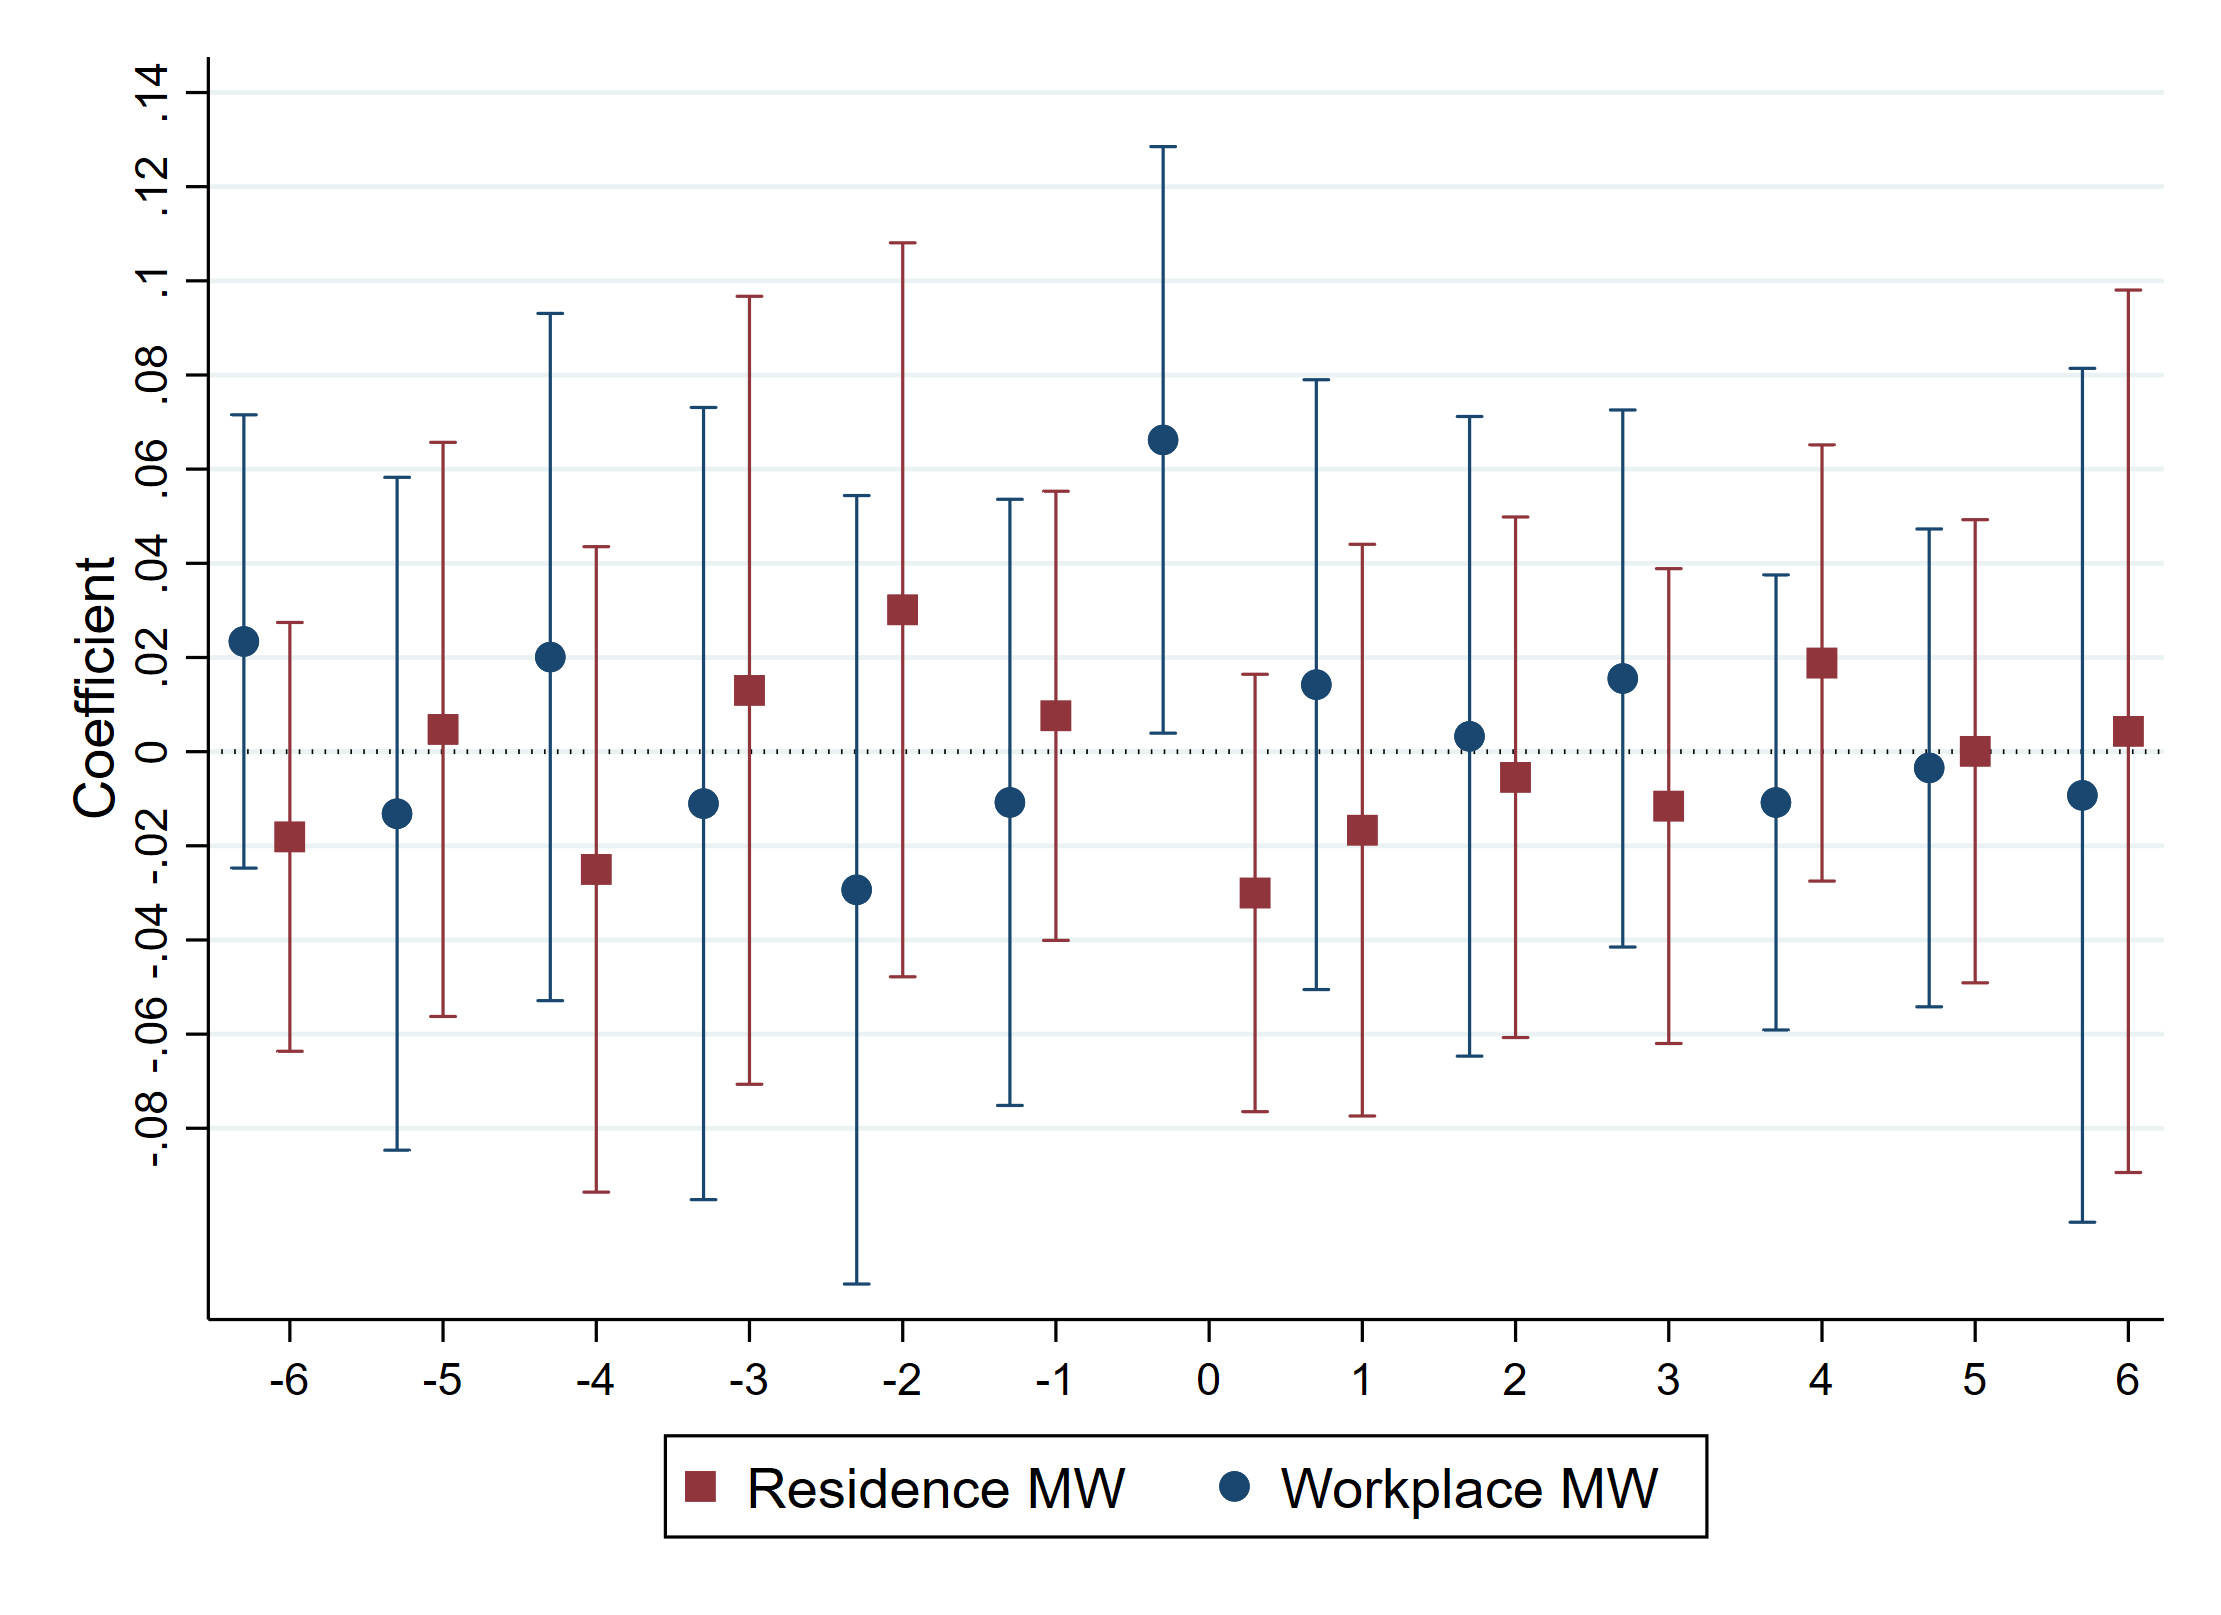
\includegraphics[width=0.68\textwidth]{fd_baseline/output/fd_both_dynamic.png}
    \end{figure}
    
    \hyperlink{dyn_baseline_plot}{\beamerbutton{Go Back}}
\end{frame}

\begin{frame}[label = wages_results]
    \frametitle{Estimates of the effect of the MW on total wages in a ZIP code}

    \vspace{2mm}
    \begin{table}[hbt!]
    \centering
    \label{tab:static_wages}

    \scalebox{0.87}{
    \begin{tabular}{@{}lccccc@{}}
        \toprule
                                & \multicolumn{4}{c}{Log total wages}
                                & \multicolumn{1}{c}{Log dividends}                        \\ \cmidrule(lr){2-5}\cmidrule(lr){6-6}
                                & (1)       & (2)      & (3)      & (4)       & (5)        \\ \midrule
        Workplace MW            & 0.1275       & 0.0909      & 0.1013      & 0.1013       & 0.0169        \\
                                & (0.0522)     & (0.0336)    & (0.0274)    & (0.0272)     & (0.0653)      \\ \midrule
        Sample                  & All       & All      & All      & Baseline  & All        \\
        Economic controls       & No        & Yes      & Yes      & Yes       & Yes        \\
        CBSA $\times$ year FE   & No        & No       & Yes      & Yes       & Yes        \\
        Within R-squared        & 0.0216       & 0.0090      & 0.0158      & 0.0953       & 0.0165        \\
        Observations            & 0      & 0     & 163,417     & 146,824      & 146,759       \\ \bottomrule
    \end{tabular}
    }
\end{table}


    
    \vspace{2mm}
    {\footnotesize
    Notes: unit of observation is ZIP code by year pairs. 
    All regressions include ZIP code FE and year FE.
    Workplace MW measure is yearly average of monthly 2017 variable.}

    \vspace{2mm}
    \hyperlink{share_pocketed_model}{\beamerbutton{Go back}}
\end{frame}

\begin{frame}[label = changes_mw_measures]
    \vspace{-3.5mm}
    
    \begin{figure}
        \begin{subfigure}{0.5\textwidth}
            \caption*{Residence MW}
            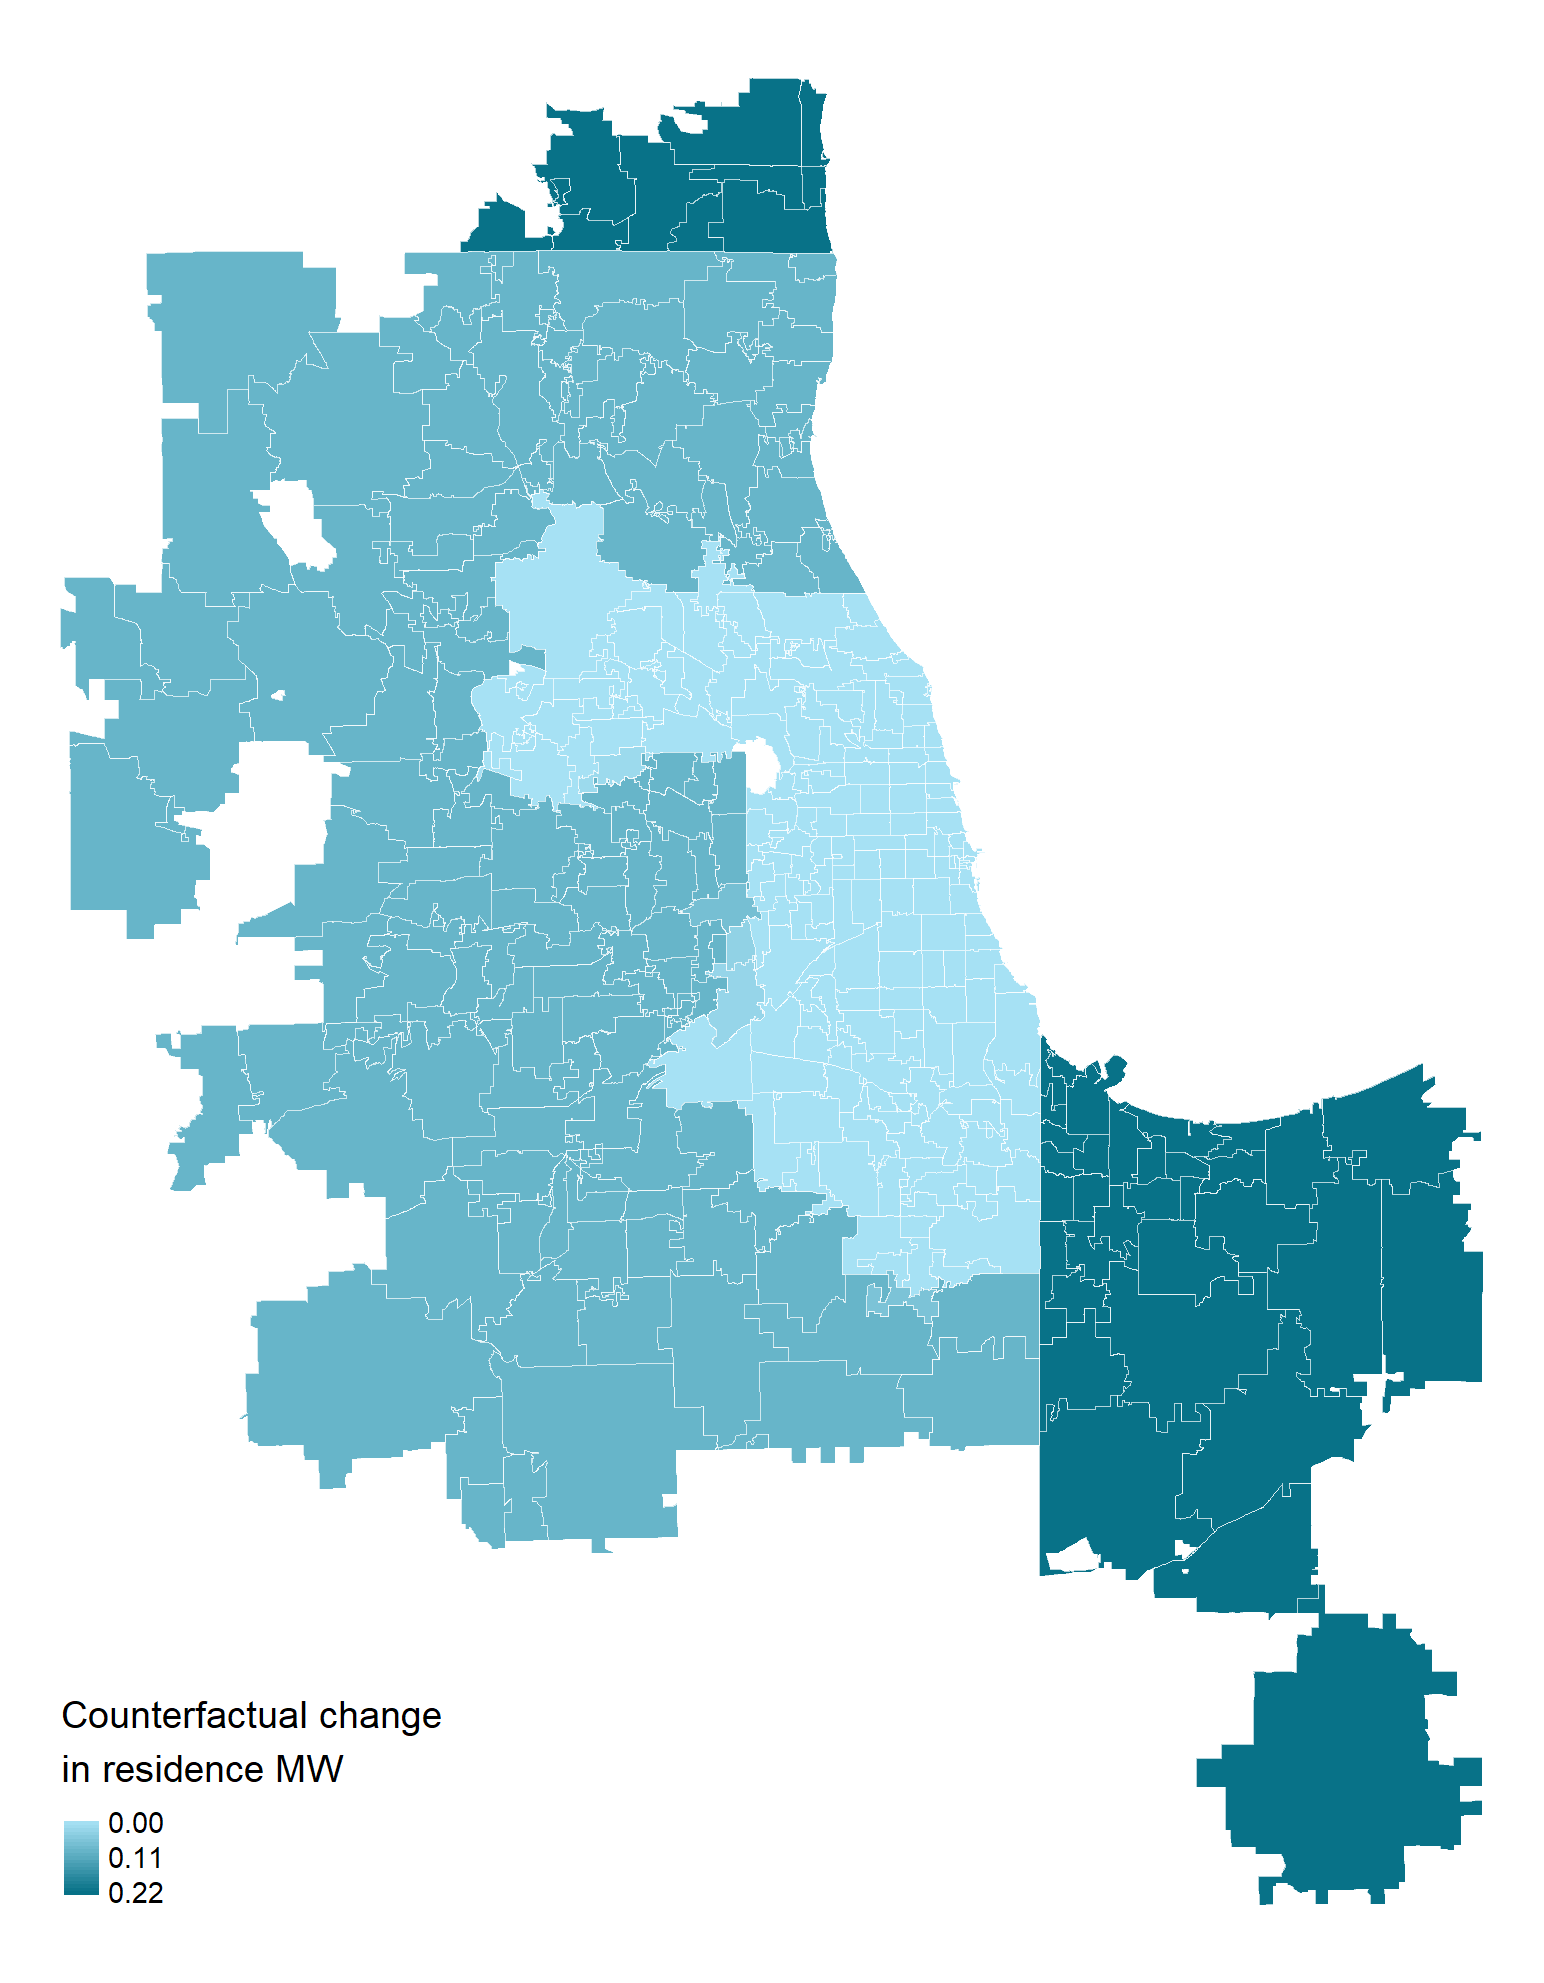
\includegraphics[width = 0.83\textwidth]{counterfactuals/output/chicago_d_mw_res.png}
        \end{subfigure}%
        \begin{subfigure}{0.5\textwidth}
            \caption*{Workplace MW}
            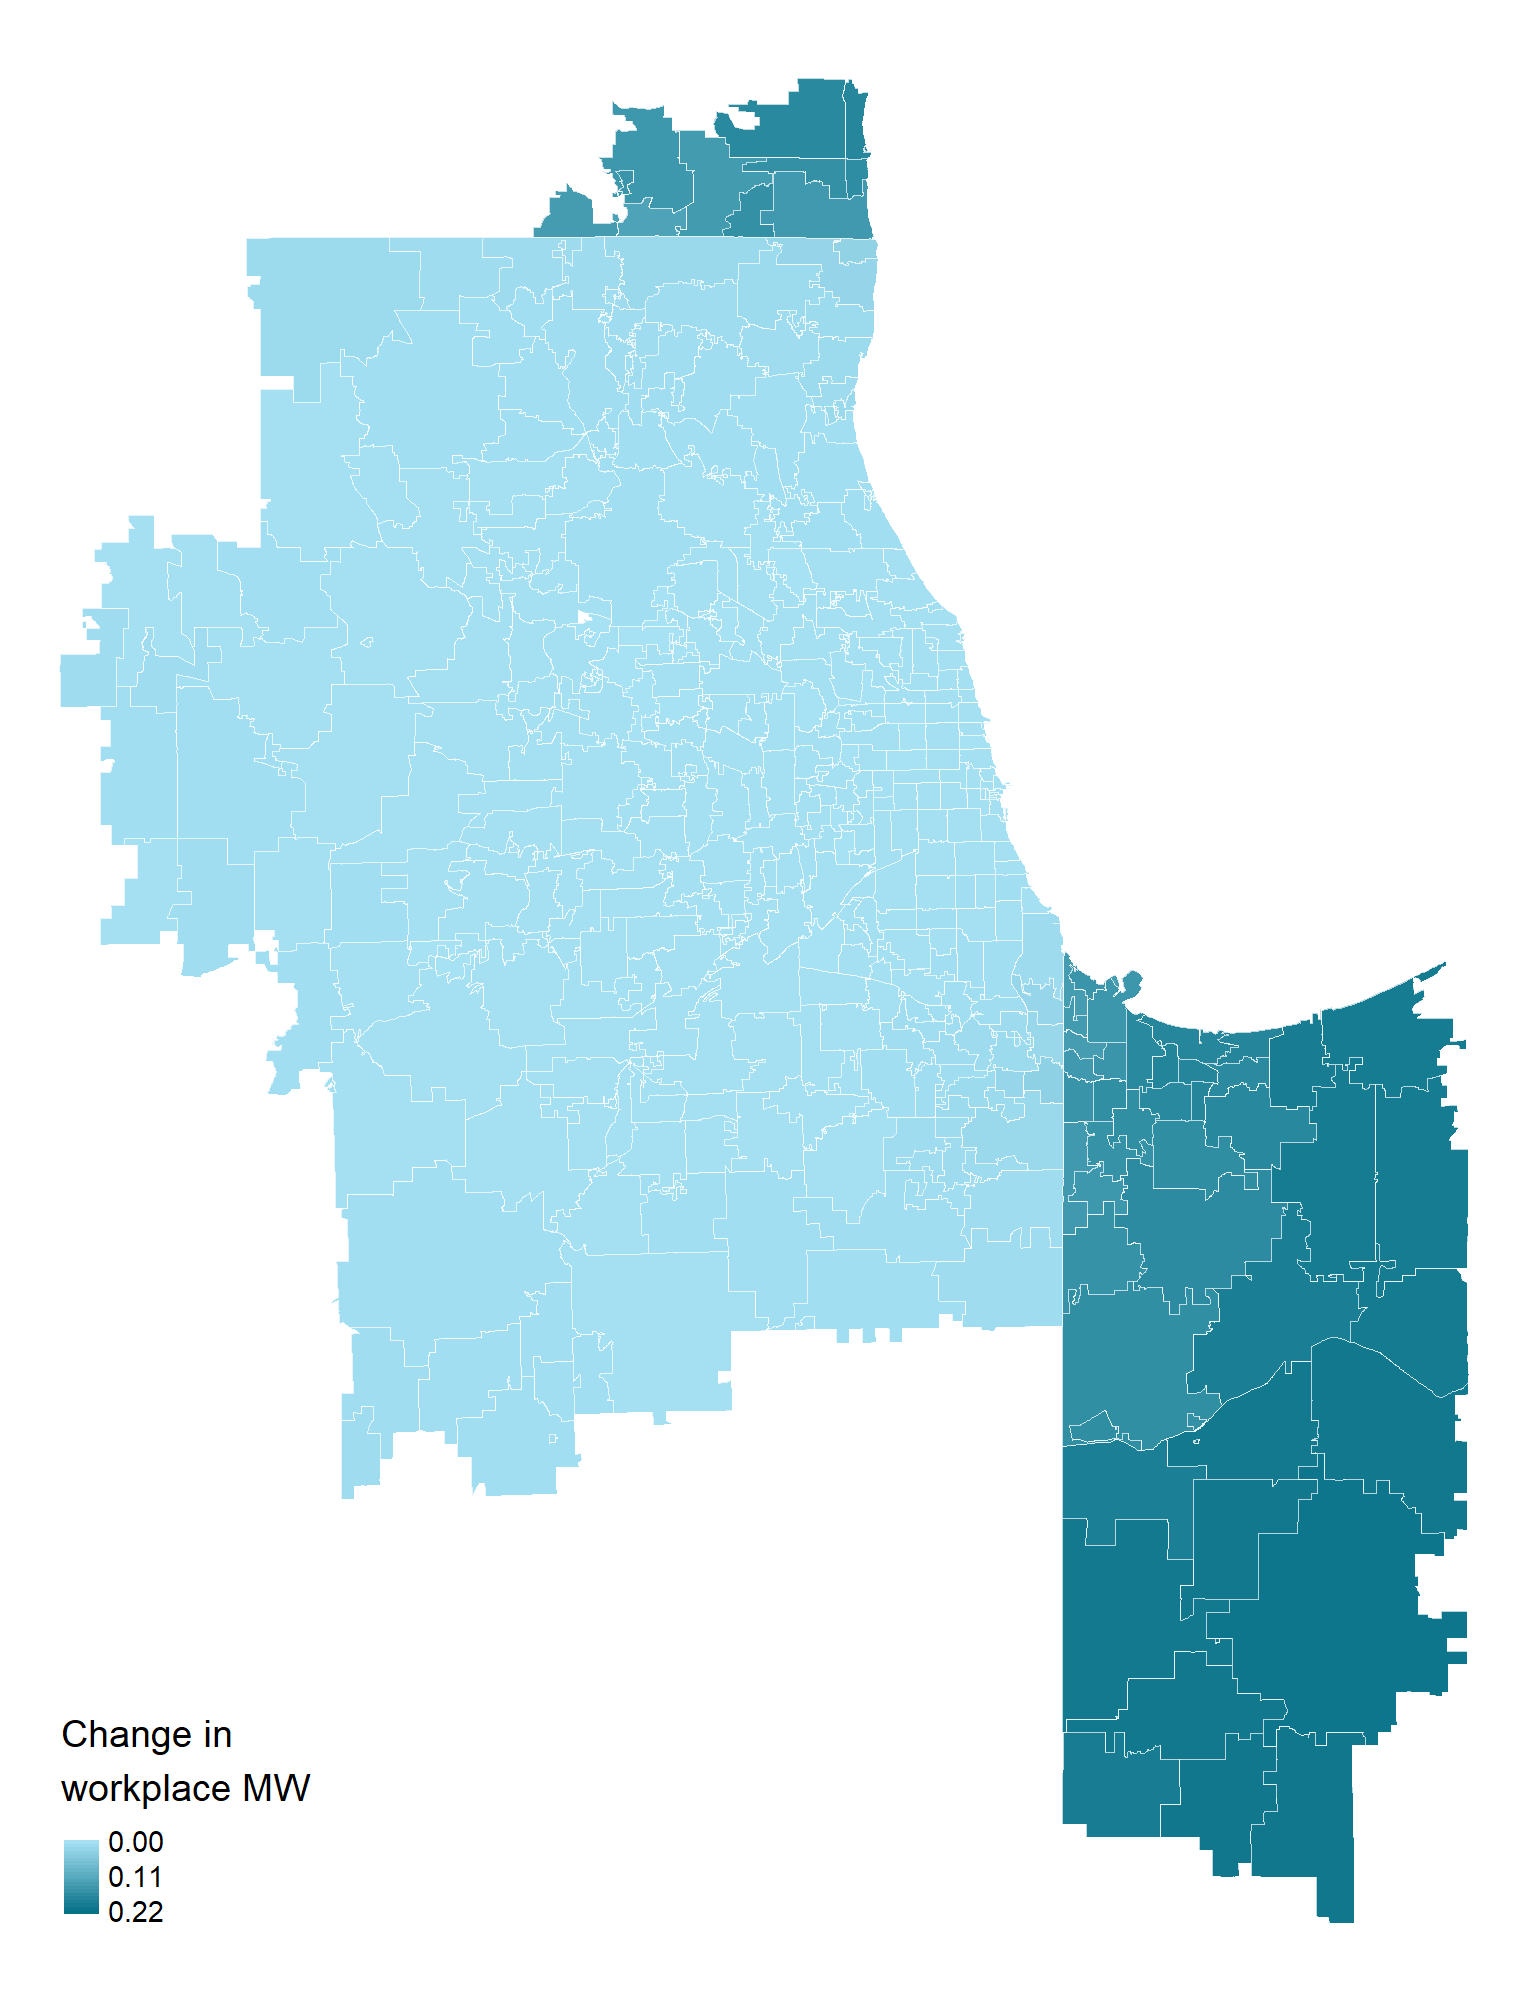
\includegraphics[width = 0.83\textwidth]{counterfactuals/output/chicago_d_mw_wkp.png}
        \end{subfigure}
    \end{figure}
    
    \vspace{-1.5mm}
    \centering
    \hyperlink{share_pocketed}{\beamerbutton{Go back}}
\end{frame}

\begin{frame}[label = changes_rents_inc]
    \vspace{-3.5mm}

    \begin{figure}
        \begin{subfigure}{0.5\textwidth}
            \caption*{Changes in log rents per sqft.}
            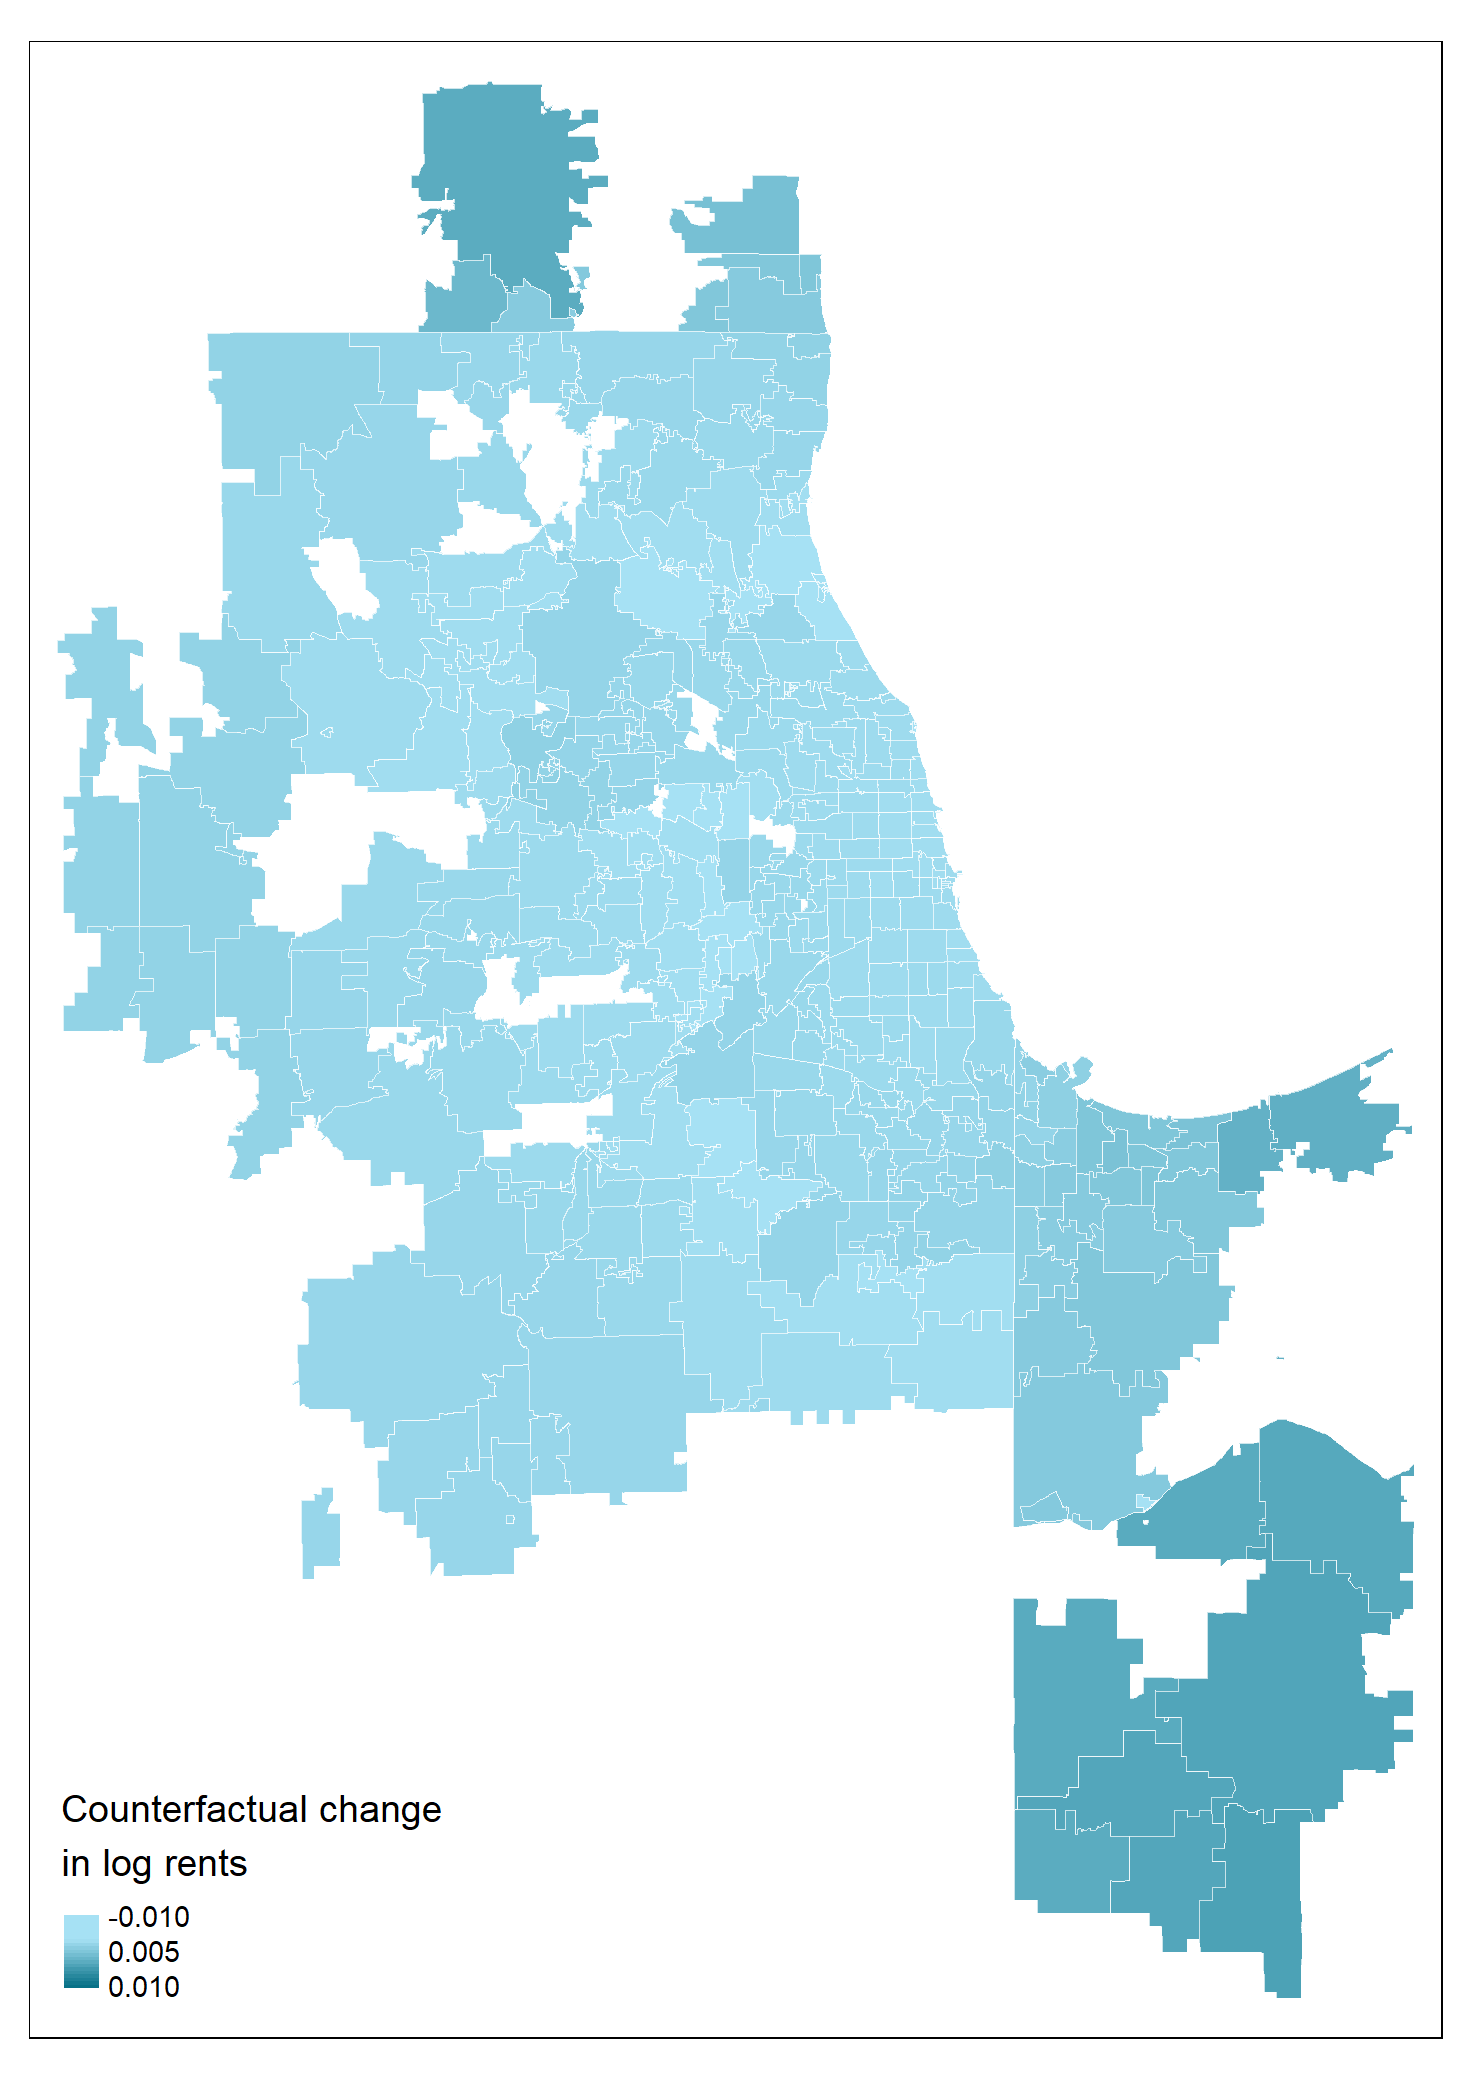
\includegraphics[width = 0.83\textwidth]{counterfactuals/output/chicago_d_ln_rents.png}
        \end{subfigure}%
        \begin{subfigure}{0.5\textwidth}
            \caption*{Changes in log total wages}
            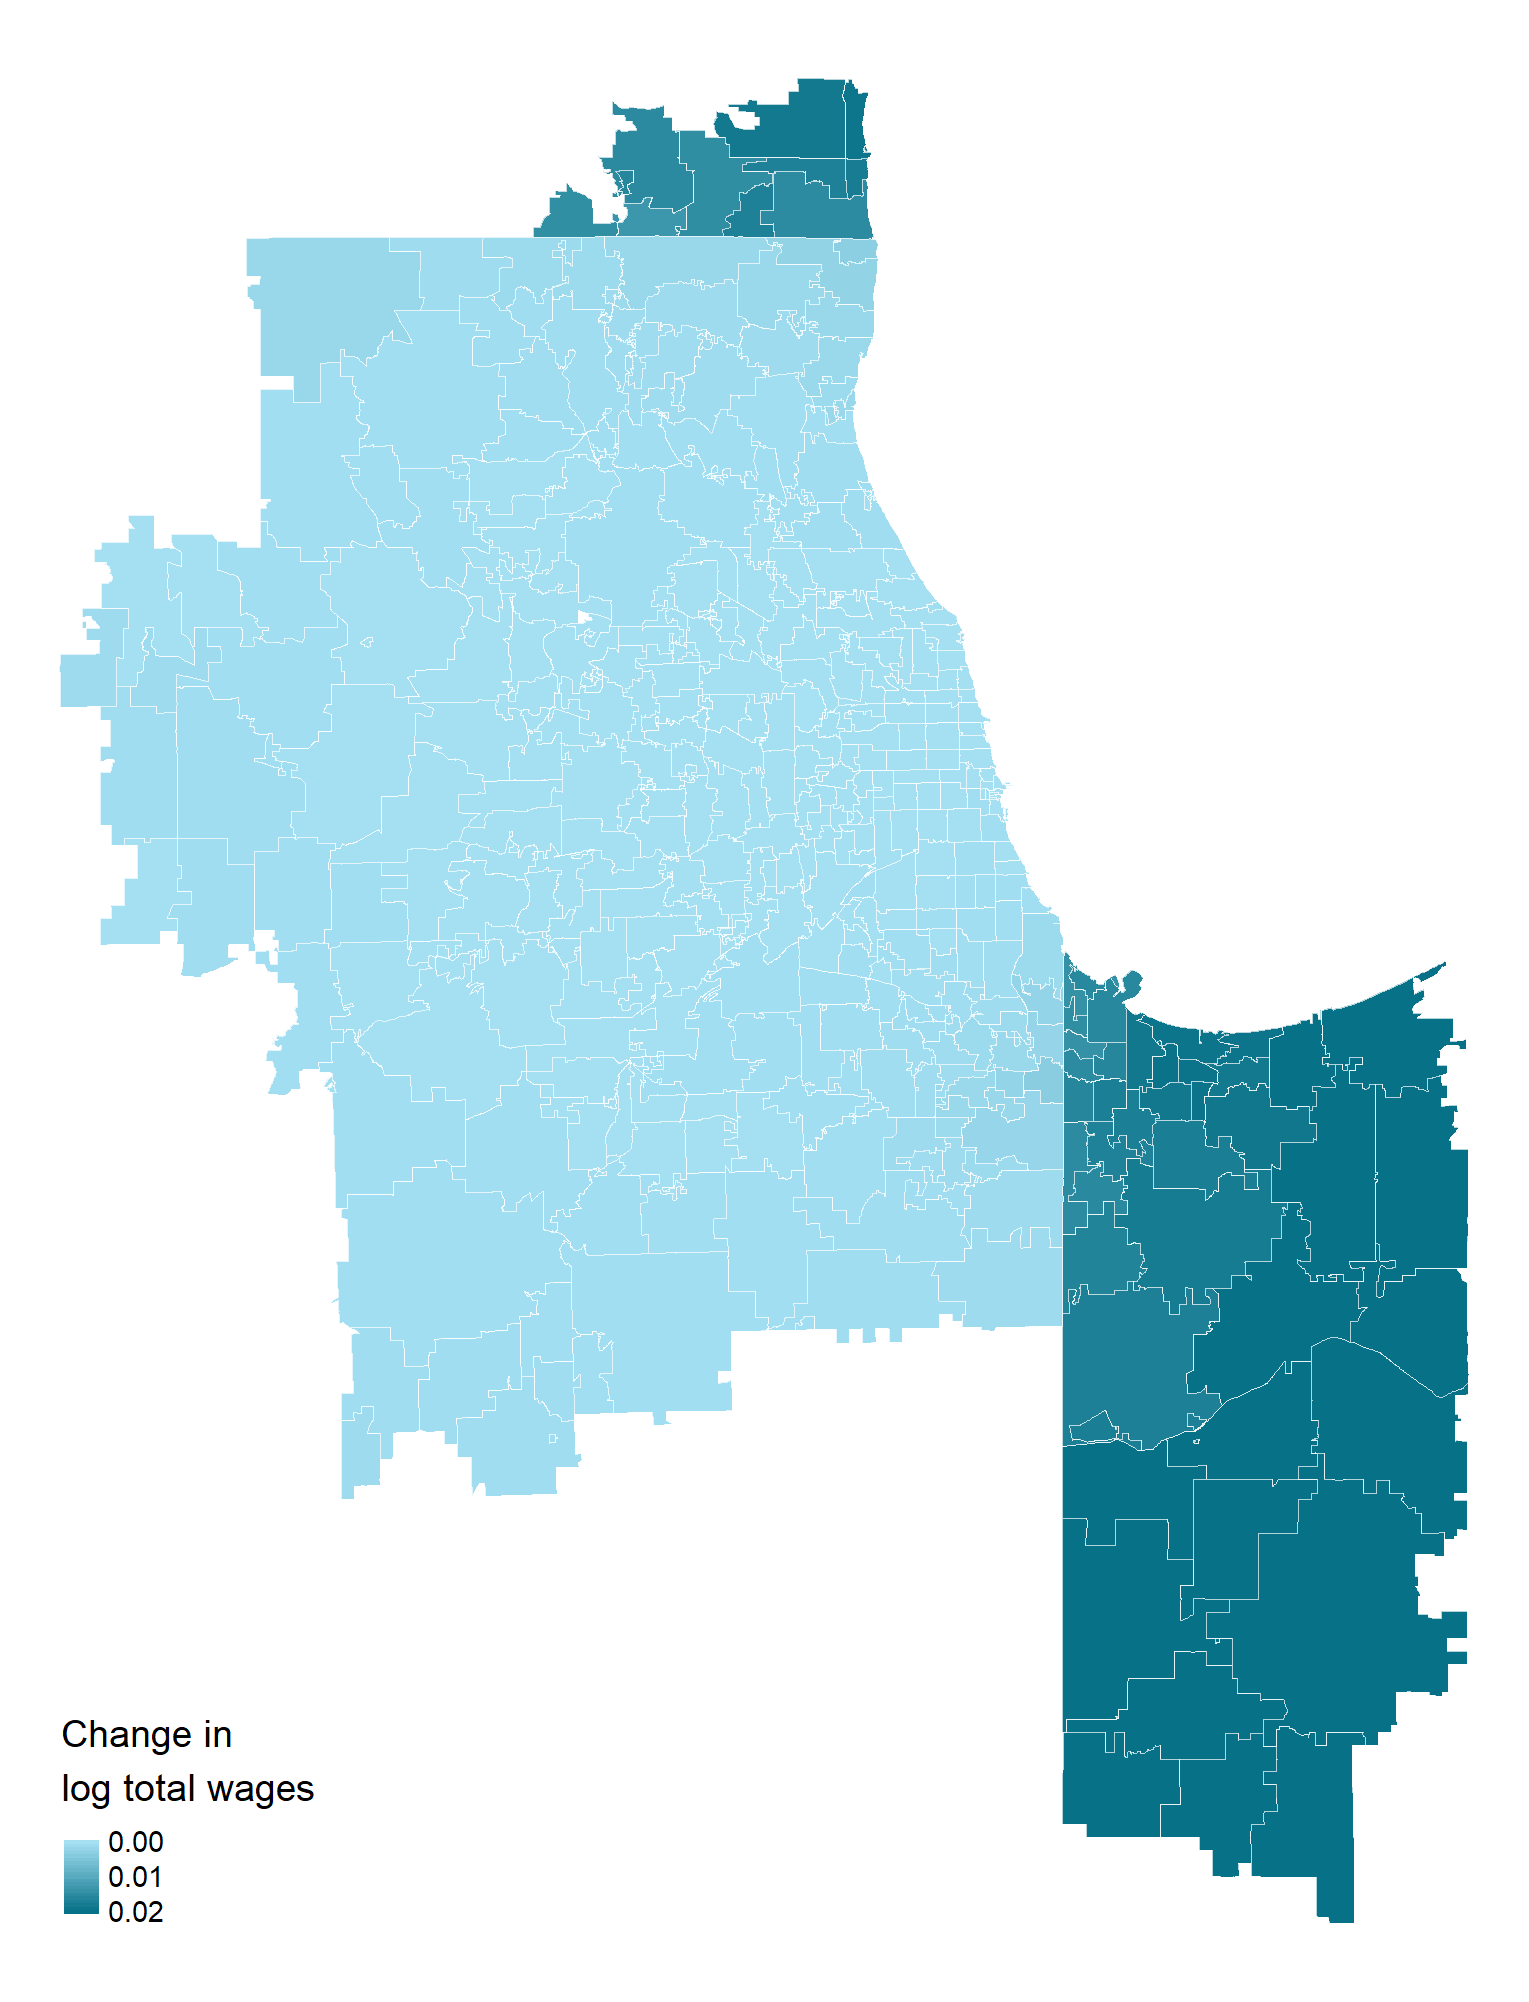
\includegraphics[width = 0.83\textwidth]{counterfactuals/output/chicago_d_ln_wagebill.png}
        \end{subfigure}
    \end{figure}
    
    \vspace{-1.5mm}
    \centering
    \hyperlink{share_pocketed}{\beamerbutton{Go back}}
\end{frame}

\end{document}